
%% bare_jrnl.tex
%% V1.4b
%% 2015/08/26
%% by Michael Shell
%% see http://www.michaelshell.org/
%% for current contact information.
%%
%% This is a skeleton file demonstrating the use of IEEEtran.cls
%% (requires IEEEtran.cls version 1.8b or later) with an IEEE
%% journal paper.
%%
%% Support sites:
%% http://www.michaelshell.org/tex/ieeetran/
%% http://www.ctan.org/pkg/ieeetran
%% and
%% http://www.ieee.org/

%%*************************************************************************
%% Legal Notice:
%% This code is offered as-is without any warranty either expressed or
%% implied; without even the implied warranty of MERCHANTABILITY or
%% FITNESS FOR A PARTICULAR PURPOSE! 
%% User assumes all risk.
%% In no event shall the IEEE or any contributor to this code be liable for
%% any damages or losses, including, but not limited to, incidental,
%% consequential, or any other damages, resulting from the use or misuse
%% of any information contained here.
%%
%% All comments are the opinions of their respective authors and are not
%% necessarily endorsed by the IEEE.
%%
%% This work is distributed under the LaTeX Project Public License (LPPL)
%% ( http://www.latex-project.org/ ) version 1.3, and may be freely used,
%% distributed and modified. A copy of the LPPL, version 1.3, is included
%% in the base LaTeX documentation of all distributions of LaTeX released
%% 2003/12/01 or later.
%% Retain all contribution notices and credits.
%% ** Modified files should be clearly indicated as such, including  **
%% ** renaming them and changing author support contact information. **
%%*************************************************************************


% *** Authors should verify (and, if needed, correct) their LaTeX system  ***
% *** with the testflow diagnostic prior to trusting their LaTeX platform ***
% *** with production work. The IEEE's font choices and paper sizes can   ***
% *** trigger bugs that do not appear when using other class files.       ***                          ***
% The testflow support page is at:
% http://www.michaelshell.org/tex/testflow/



\documentclass[letterpaper,journal]{IEEEtran}
% \usepackage[letterpaper, top=1.92cm, bottom=3.2cm, left=1.92cm, right=1.92cm]{geometry}
%
% If IEEEtran.cls has not been installed into the LaTeX system files,
% manually specify the path to it like:
% \documentclass[journal]{../sty/IEEEtran}
% \usepackage{multirow}
\usepackage{graphicx}
% \usepackage{float}
% \usepackage[compact]{titlesec}
% \usepackage{subfig}
\usepackage{amssymb}
\usepackage{setspace} % 用于调整行距



% \usepackage{soul}
% \usepackage{subcaption}
\usepackage{booktabs}
\usepackage{booktabs,makecell,multirow}
%\usepackage{algorithm}
%\usepackage{algorithmic}
%\usepackage{subfig}%多个子图
% \usepackage{caption}%注释设置
% \newcommand\MYhyperrefoptions{bookmarks=true,bookmarksnumbered=true,
% pdfpagemode={UseOutlines},plainpages=false,pdfpagelabels=true,
% colorlinks=true,linkcolor={black},citecolor={black},urlcolor={black},
% pdftitle={Bare Demo of IEEEtran.cls for Computer Society Journals},%<!CHANGE!
% pdfsubject={Typesetting},%<!CHANGE!
% pdfauthor={Michael D. Shell},%<!CHANGE!
% pdfkeywords={Computer Society, IEEEtran, journal, LaTeX, paper,
%              template}}%<^!CHANGE!


% correct bad hyphenation here
% \hyphenation{op-tical net-works semi-conduc-tor}
\usepackage{booktabs}
\usepackage{hyperref}

\usepackage{widetext}
%\usepackage{algorithm}
%\usepackage{algorithmic}
\usepackage{bm}
\usepackage{color, xcolor}
\usepackage{transparent}
% \usepackage{graphicx}
\usepackage{import}
\usepackage[ruled]{algorithm2e}
\usepackage{amsmath}
\usepackage{amsthm}
\allowdisplaybreaks[4]
\usepackage{algorithmic}
\makeatletter
\newcommand{\rmnum}[1]{\romannumeral #1}
\newcommand{\Rmnum}[1]{\expandafter\@slowromancap\romannumeral #1@}
\makeatother
% \usepackage{graphicx}
\newcommand{\rs}{\!\!}
% \usepackage{subfloat} 
\usepackage{subfigure} 
\usepackage{threeparttable}


%\usepackage{algorithm}  
%\usepackage{algpseudocode}  
%\usepackage{amsmath}  
%\renewcommand{\algorithmicrequire}{\textbf{Input:}}  % Use Input in the format of Algorithm  
%\renewcommand{\algorithmicensure}{\textbf{Output:}} % Use Output in the format of Algorithm  

%\makeatletter  
%\newif\if@restonecol  
%\makeatother  
%\let\algorithm\relax  
%\let\endalgorithm\relax  
%\usepackage[linesnumbered,ruled,vlined]{algorithm2e}%[ruled,vlined]{  
%\usepackage{algpseudocode}  
%\usepackage{amsmath}  
%\renewcommand{\algorithmicrequire}{\textbf{Input:}}  % Use Input in the format of Algorithm  
%\renewcommand{\algorithmicensure}{\textbf{Output:}} % Use Output in the format of Algorithm   


% Some very useful LaTeX packages include:
% (uncomment the ones you want to load)


% *** MISC UTILITY PACKAGES ***
%
%\usepackage{ifpdf}
% Heiko Oberdiek's ifpdf.sty is very useful if you need conditional
% compilation based on whether the output is pdf or dvi.
% usage:
% \ifpdf
%   % pdf code
% \else
%   % dvi code
% \fi
% The latest version of ifpdf.sty can be obtained from:
% http://www.ctan.org/pkg/ifpdf
% Also, note that IEEEtran.cls V1.7 and later provides a builtin
% \ifCLASSINFOpdf conditional that works the same way.
% When switching from latex to pdflatex and vice-versa, the compiler may
% have to be run twice to clear warning/error messages.






% *** CITATION PACKAGES ***
%
%\usepackage{cite}
% cite.sty was written by Donald Arseneau
% V1.6 and later of IEEEtran pre-defines the format of the cite.sty package
% \cite{} output to follow that of the IEEE. Loading the cite package will
% result in citation numbers being automatically sorted and properly
% "compressed/ranged". e.g., [1], [9], [2], [7], [5], [6] without using
% cite.sty will become [1], [2], [5]--[7], [9] using cite.sty. cite.sty's
% \cite will automatically add leading space, if needed. Use cite.sty's
% noadjust option (cite.sty V3.8 and later) if you want to turn this off
% such as if a citation ever needs to be enclosed in parenthesis.
% cite.sty is already installed on most LaTeX systems. Be sure and use
% version 5.0 (2009-03-20) and later if using hyperref.sty.
% The latest version can be obtained at:
% http://www.ctan.org/pkg/cite
% The documentation is contained in the cite.sty file itself.


\usepackage{color}
\usepackage{transparent}
\usepackage{graphicx}
\usepackage{import}


\newtheorem{proposition}{Proposition}
\newtheorem{theorem}{Theorem}
% \usepackage{ntheorem}
% \newtheorem{proof}{Proof}
\newtheorem{thm}{\bf Theorem}
\newtheorem{corollary}{\bf Corollary}
\newtheorem{lemma}{Lemma}
%\newtheorem{lemma}{\bf Lemma}
\newtheorem{assumption}{\bf Assumption}
% *** GRAPHICS RELATED PACKAGES ***
%
\ifCLASSINFOpdf
  % \usepackage[pdftex]{graphicx}
  % declare the path(s) where your graphic files are
  % \graphicspath{{../pdf/}{../jpeg/}}
  % and their extensions so you won't have to specify these with
  % every instance of \includegraphics
  % \DeclareGraphicsExtensions{.pdf,.jpeg,.png}
\else
  % or other class option (dvipsone, dvipdf, if not using dvips). graphicx
  % will default to the driver specified in the system graphics.cfg if no
  % driver is specified.
  % \usepackage[dvips]{graphicx}
  % declare the path(s) where your graphic files are
  % \graphicspath{{../eps/}}
  % and their extensions so you won't have to specify these with
  % every instance of \includegraphics
  % \DeclareGraphicsExtensions{.eps}
\fi
% graphicx was written by David Carlisle and Sebastian Rahtz. It is
% required if you want graphics, photos, etc. graphicx.sty is already
% installed on most LaTeX systems. The latest version and documentation
% can be obtained at: 
% http://www.ctan.org/pkg/graphicx
% Another good source of documentation is "Using Imported Graphics in
% LaTeX2e" by Keith Reckdahl which can be found at:
% http://www.ctan.org/pkg/epslatex
%
% latex, and pdflatex in dvi mode, support graphics in encapsulated
% postscript (.eps) format. pdflatex in pdf mode supports graphics
% in .pdf, .jpeg, .png and .mps (metapost) formats. Users should ensure
% that all non-photo figures use a vector format (.eps, .pdf, .mps) and
% not a bitmapped formats (.jpeg, .png). The IEEE frowns on bitmapped formats
% which can result in "jaggedy"/blurry rendering of lines and letters as
% well as large increases in file sizes.
%
% You can find documentation about the pdfTeX application at:
% http://www.tug.org/applications/pdftex





% *** MATH PACKAGES ***
%
%\usepackage{amsmath}
% A popular package from the American Mathematical Society that provides
% many useful and powerful commands for dealing with mathematics.
%
% Note that the amsmath package sets \interdisplaylinepenalty to 10000
% thus preventing page breaks from occurring within multiline equations. Use:
%\interdisplaylinepenalty=2500
% after loading amsmath to restore such page breaks as IEEEtran.cls normally
% does. amsmath.sty is already installed on most LaTeX systems. The latest
% version and documentation can be obtained at:
% http://www.ctan.org/pkg/amsmath





% *** SPECIALIZED LIST PACKAGES ***
%
%\usepackage{algorithmic}
% algorithmic.sty was written by Peter Williams and Rogerio Brito.
% This package provides an algorithmic environment fo describing algorithms.
% You can use the algorithmic environment in-text or within a figure
% environment to provide for a floating algorithm. Do NOT use the algorithm
% floating environment provided by algorithm.sty (by the same authors) or
% algorithm2e.sty (by Christophe Fiorio) as the IEEE does not use dedicated
% algorithm float types and packages that provide these will not provide
% correct IEEE style captions. The latest version and documentation of
% algorithmic.sty can be obtained at:
% http://www.ctan.org/pkg/algorithms
% Also of interest may be the (relatively newer and more customizable)
% algorithmicx.sty package by Szasz Janos:
% http://www.ctan.org/pkg/algorithmicx




% *** ALIGNMENT PACKAGES ***
%
%\usepackage{array}
% Frank Mittelbach's and David Carlisle's array.sty patches and improves
% the standard LaTeX2e array and tabular environments to provide better
% appearance and additional user controls. As the default LaTeX2e table
% generation code is lacking to the point of almost being broken with
% respect to the quality of the end results, all users are strongly
% advised to use an enhanced (at the very least that provided by array.sty)
% set of table tools. array.sty is already installed on most systems. The
% latest version and documentation can be obtained at:
% http://www.ctan.org/pkg/array


% IEEEtran contains the IEEEeqnarray family of commands that can be used to
% generate multiline equations as well as matrices, tables, etc., of high
% quality.




% *** SUBFIGURE PACKAGES ***
%\ifCLASSOPTIONcompsoc
%  \usepackage[caption=false,font=normalsize,labelfont=sf,textfont=sf]{subfig}
%\else
%  \usepackage[caption=false,font=footnotesize]{subfig}
%\fi
% subfig.sty, written by Steven Douglas Cochran, is the modern replacement
% for subfigure.sty, the latter of which is no longer maintained and is
% incompatible with some LaTeX packages including fixltx2e. However,
% subfig.sty requires and automatically loads Axel Sommerfeldt's caption.sty
% which will override IEEEtran.cls' handling of captions and this will result
% in non-IEEE style figure/table captions. To prevent this problem, be sure
% and invoke subfig.sty's "caption=false" package option (available since
% subfig.sty version 1.3, 2005/06/28) as this is will preserve IEEEtran.cls
% handling of captions.
% Note that the Computer Society format requires a larger sans serif font
% than the serif footnote size font used in traditional IEEE formatting
% and thus the need to invoke different subfig.sty package options depending
% on whether compsoc mode has been enabled.
%
% The latest version and documentation of subfig.sty can be obtained at:
% http://www.ctan.org/pkg/subfig




% *** FLOAT PACKAGES ***
%
%\usepackage{fixltx2e}
% fixltx2e, the successor to the earlier fix2col.sty, was written by
% Frank Mittelbach and David Carlisle. This package corrects a few problems
% in the LaTeX2e kernel, the most notable of which is that in current
% LaTeX2e releases, the ordering of single and double column floats is not
% guaranteed to be preserved. Thus, an unpatched LaTeX2e can allow a
% single column figure to be placed prior to an earlier double column
% figure.
% Be aware that LaTeX2e kernels dated 2015 and later have fixltx2e.sty's
% corrections already built into the system in which case a warning will
% be issued if an attempt is made to load fixltx2e.sty as it is no longer
% needed.
% The latest version and documentation can be found at:
% http://www.ctan.org/pkg/fixltx2e


%\usepackage{stfloats}
% stfloats.sty was written by Sigitas Tolusis. This package gives LaTeX2e
% the ability to do double column floats at the bottom of the page as well
% as the top. (e.g., "\begin{figure*}[!b]" is not normally possible in
% LaTeX2e). It also provides a command:
%\fnbelowfloat
% to enable the placement of footnotes below bottom floats (the standard
% LaTeX2e kernel puts them above bottom floats). This is an invasive package
% which rewrites many portions of the LaTeX2e float routines. It may not work
% with other packages that modify the LaTeX2e float routines. The latest
% version and documentation can be obtained at:
% http://www.ctan.org/pkg/stfloats
% Do not use the stfloats baselinefloat ability as the IEEE does not allow
% \baselineskip to stretch. Authors submitting work to the IEEE should note
% that the IEEE rarely uses double column equations and that authors should try
% to avoid such use. Do not be tempted to use the cuted.sty or midfloat.sty
% packages (also by Sigitas Tolusis) as the IEEE does not format its papers in
% such ways.
% Do not attempt to use stfloats with fixltx2e as they are incompatible.
% Instead, use Morten Hogholm'a dblfloatfix which combines the features
% of both fixltx2e and stfloats:
%
% \usepackage{dblfloatfix}
% The latest version can be found at:
% http://www.ctan.org/pkg/dblfloatfix




%\ifCLASSOPTIONcaptionsoff
%  \usepackage[nomarkers]{endfloat}
% \let\MYoriglatexcaption\caption
% \renewcommand{\caption}[2][\relax]{\MYoriglatexcaption[#2]{#2}}
%\fi
% endfloat.sty was written by James Darrell McCauley, Jeff Goldberg and 
% Axel Sommerfeldt. This package may be useful when used in conjunction with 
% IEEEtran.cls'  captionsoff option. Some IEEE journals/societies require that
% submissions have lists of figures/tables at the end of the paper and that
% figures/tables without any captions are placed on a page by themselves at
% the end of the document. If needed, the draftcls IEEEtran class option or
% \CLASSINPUTbaselinestretch interface can be used to increase the line
% spacing as well. Be sure and use the nomarkers option of endfloat to
% prevent endfloat from "marking" where the figures would have been placed
% in the text. The two hack lines of code above are a slight modification of
% that suggested by in the endfloat docs (section 8.4.1) to ensure that
% the full captions always appear in the list of figures/tables - even if
% the user used the short optional argument of \caption[]{}.
% IEEE papers do not typically make use of \caption[]'s optional argument,
% so this should not be an issue. A similar trick can be used to disable
% captions of packages such as subfig.sty that lack options to turn off
% the subcaptions:
% For subfig.sty:
% \let\MYorigsubfloat\subfloat
% \renewcommand{\subfloat}[2][\relax]{\MYorigsubfloat[]{#2}}
% However, the above trick will not work if both optional arguments of
% the \subfloat command are used. Furthermore, there needs to be a
% description of each subfigure *somewhere* and endfloat does not add
% subfigure captions to its list of figures. Thus, the best approach is to
% avoid the use of subfigure captions (many IEEE journals avoid them anyway)
% and instead reference/explain all the subfigures within the main caption.
% The latest version of endfloat.sty and its documentation can obtained at:
% http://www.ctan.org/pkg/endfloat
%
% The IEEEtran \ifCLASSOPTIONcaptionsoff conditional can also be used
% later in the document, say, to conditionally put the References on a 
% page by themselves.




% *** PDF, URL AND HYPERLINK PACKAGES ***
%
%\usepackage{url}
% url.sty was written by Donald Arseneau. It provides better support for
% handling and breaking URLs. url.sty is already installed on most LaTeX
% systems. The latest version and documentation can be obtained at:
% http://www.ctan.org/pkg/url
% Basically, \url{my_url_here}.




% *** Do not adjust lengths that control margins, column widths, etc. ***
% *** Do not use packages that alter fonts (such as pslatex).         ***
% There should be no need to do such things with IEEEtran.cls V1.6 and later.
% (Unless specifically asked to do so by the journal or conference you plan
% to submit to, of course. )


% correct bad hyphenation here
\hyphenation{op-tical net-works semi-conduc-tor}
 \usepackage{graphicx}
\usepackage{CJKutf8}
\usepackage{bm}
\usepackage{cite}
\usepackage{amssymb}
\usepackage{amsmath}
 \usepackage{threeparttable}
\begin{document}
	\begin{CJK}{UTF8}{gbsn}
%
% paper title
% Titles are generally capitalized except for words such as a, an, and, as,
% at, but, by, for, in, nor, of, on, or, the, to and up, which are usually
% not capitalized unless they are the first or last word of the title.
% Linebreaks \\ can be used within to get better formatting as desired.
% Do not put math or special symbols in the title.
%\title{Underwater Differential Game: DRL-Assisted Target Hunting Task with Communication Delay}
\title{Optimizing Split Federated Learning with Unstable Client Participation}
%
%
% author names and IEEE memberships
% note positions of commas and nonbreaking spaces ( ~ ) LaTeX will not break
% a structure at a ~ so this keeps an author's name from being broken across
% two lines.
% use \thanks{} to gain access to the first footnote area
% a separate \thanks must be used for each paragraph as LaTeX2e's \thanks
% was not built to handle multiple paragraphs
%

%\author{Wei Wei,~\IEEEmembership{Student Member,~IEEE,}
%	Jingjing~Wang,~\IEEEmembership{Senior Member,~IEEE,}
%	Jun~Du,~\IEEEmembership{Senior Member,~IEEE,}
%	Zhengru~Fang,~\IEEEmembership{Student Member,~IEEE,}
%	~Yong~Ren,~\IEEEmembership{Senior Member,~IEEE}
%	and~C. L. Philip Chen,~\IEEEmembership{Fellow,~IEEE}
%	
%	%      and~Yong~Ren,~\IEEEmembership{Life~Fellow,~IEEE}% <-this % stops a space
%	%\vspace{-1.4em}
%	\thanks{W. Wei is with the Department of Electrical and Electronic Engineering, the University of Hong Kong, Hong Kong, 999077, China. E-mail: weiwei2020214906@gmail.com.}% <-this % stops a space
%	\thanks{J. Wang is with the School of Cyber Science and Technology, Beihang University, Beijing, 100191, China. E-mail: chinaeephd@gmail.com (Corresponding author).}
%	\thanks{ J. Du and Y. Ren are with the Department of Electronic Engineering, Tsinghua University, Beijing, 100084, China. Y. Ren is also with Peng Cheng Laboratory, Shenzhen, 518055, China. E-mail: \{jundu,reny\}@tsinghua.edu.cn.}% <-this % stops a space
%	\thanks{ Z. Fang is with the Department of Computer Science,
%		City University of Hong Kong, Hong Kong, 999077, China. E-mail: zhefang4@cityu.edu.hk.}% <-this % stops a space
%	\thanks{C. L. Philip Chen is with the School of Computer Science and Engineering, South China University of Technology, Guangzhou, 510006, China. E-mail: Philip.Chen@ieee.org.}
%	\thanks{A preliminary version of this paper was presented at IEEE International Conference on Communications (ICC) at Seoul, Korea. }
%}% }}

% note the % following the last \IEEEmembership and also \thanks - 
% these prevent an unwanted space from occurring between the last author name
% and the end of the author line. i.e., if you had this:
% 
% \author{....lastname \thanks{...} \thanks{...} }
%                     ^------------^------------^----Do not want these spaces!
%
% a space would be appended to the last name and could cause every name on that
% line to be shifted left slightly. This is one of those "LaTeX things". For
% instance, "\textbf{A} \textbf{B}" will typeset as "A B" not "AB". To get
% "AB" then you have to do: "\textbf{A}\textbf{B}"
% \thanks is no different in this regard, so shield the last } of each \thanks
% that ends a line with a % and do not let a space in before the next \thanks.
% Spaces after \IEEEmembership other than the last one are OK (and needed) as
% you are supposed to have spaces between the names. For what it is worth,
% this is a minor point as most people would not even notice if the said evil
% space somehow managed to creep in.



% The paper headers
\markboth{IEEE Transactions on  Mobile Computing}%
% \markboth{ on Mobile Computing}%
{Shell \MakeLowercase{\textit{et al.}}: Bare Demo of IEEEtran.cls for IEEE Journals}
% The only time the second header will appear is for the odd numbered pages
% after the title page when using the twoside option.
% 
% *** Note that you probably will NOT want to include the author's ***
% *** name in the headers of peer review papers.                   ***
% You can use \ifCLASSOPTIONpeerreview for conditional compilation here if
% you desire.




% If you want to put a publisher's ID mark on the page you can do it like
% this:
%\IEEEpubid{0000--0000/00\$00.00~\copyright~2015 IEEE}
% Remember, if you use this you must call \IEEEpubidadjcol in the second
% column for its text to clear the IEEEpubid mark.



% use for special paper notices
%\IEEEspecialpapernotice{(Invited Paper)}



% make the title area
	
\author{Wei Wei,~\IEEEmembership{Graduate Student Member,~IEEE,}
	Zheng~Lin,~\IEEEmembership{Graduate 
 Student Member,~IEEE,}
 Xihui Liu,~\IEEEmembership{Member,~IEEE,}
 Hongyang~Du,~\IEEEmembership{Member,~IEEE,}
 Dusit~Niyato,~\IEEEmembership{Fellow,~IEEE,} and~Xianhao~Chen,~\IEEEmembership{Member,~IEEE}
	

\thanks{The work was supported in part by the Research Grants Council of Hong Kong under Grant 27213824 and CRS HKU702/24, in part by HKU-SCF FinTech Academy R\&D Funding, and in part by HKU IDS Research Seed Fund under Grant IDS-RSF2023-0012.  
\textit{(Corresponding author: Xianhao Chen)}
}
\thanks{ Wei Wei, Zheng Lin, Xihui Liu, Hongyang Du, and Xianhao Chen are with the Department of Electrical and Electronic Engineering, the University of Hong Kong, Pok Fu Lam, Hong Kong SAR, 999077, China. Xihui Liu and Xianhao Chen are also with the HKU Musketeers Foundation Institute of Data Science, the University of Hong Kong, Pok Fu Lam, Hong Kong SAR, 999077, China. Dusit Niyato is with the College of Computing
and Data Science, Nanyang Technological University, Singapore 639798. (e-mail: weiwei@eee.hku.hk; linzheng@eee.hku.hk; xihuiliu@eee.hku.hk; duhy@eee.hku.hk;
xchen@eee.hku.hk; dniyato@ntu.edu.sg).
}
}

 

\maketitle

% As a general rule, do not put math, special symbols or citations
% in the abstract or keywords.
\begin{abstract}
To enable training of large artificial intelligence (AI) models at the network edge, split federated learning (SFL) has emerged as a promising approach by distributing computation between edge devices and a server. However, while unstable network environments pose significant challenges to SFL, prior schemes often overlook such an effect by assuming perfect client participation, rendering them impractical for real-world scenarios. In this work, we develop an optimization framework for SFL with unstable client participation. We theoretically derive the first convergence upper bound for SFL with unstable client participation by considering activation uploading failures, gradient downloading failures, and model aggregation failures. Based on the theoretical results, we formulate a joint optimization problem for client sampling and model splitting to minimize the upper bound. We then  develop an efficient solution approach to solve the problem optimally. 
% Extensive simulations across diverse datasets demonstrate the superiority of our proposed framework.
Extensive simulations on EMNIST and CIFAR-10 demonstrate the superiority of our proposed framework  compared to existing benchmarks.
\end{abstract}

% Note that keywords are not normally used for peerreview papers.
\begin{IEEEkeywords}
Split federated learning, client sampling, model splitting, convergence analysis, optimization algorithm, wireless networks.
\end{IEEEkeywords}



% For peer review papers, you can put extra information on the cover
% page as needed:
% \ifCLASSOPTIONpeerreview
% \begin{center} \bfseries EDICS Category: 3-BBND \end{center}
% \fi
%
% For peerreview papers, this IEEEtran command inserts a page break and
% creates the second title. It will be ignored for other modes.
\IEEEpeerreviewmaketitle
% \pagestyle{empty}  % no page number for the second and the later pages
% \thispagestyle{empty} % no page number for the first page
\section{Introduction}
Edge learning enables artificial intelligence (AI) computation close to the data source, enhancing privacy, saving bandwidth, and enabling personalization of edge devices~\cite{Edge-AI-Technology-Report, 10843329, 10040976,wei2025pipeliningsplitlearningmultihop, ZW_spectrum,9944188,9839238,10298247}. However, the rapid expansion of AI models presents unprecedented computational challenges. State-of-the-art models are inherently incompatible with the limited hardware resources of edge devices or servers. For instance, edge devices such as the NVIDIA Jetson AGX Xavier with 16 GB of RAM struggle to train models that exceed 50-million parameters with full precision \cite{jetson-agx}. Given these challenges, split federated learning (SFL)~\cite{vepakomma2018split, lin2023split,10934144}, which utilizes a client-edge server architecture, presents a promising solution. In SFL, the AI model is divided into two segments: the initial layers are trained on clients over local data, whereas the subsequent layers are trained on a server that provides more powerful computing resources~\cite{lin2024efficient,lin2025leo}. Moreover, a federated server (or simply Fed server) periodically aggregates client-side sub-models, akin to federated learning (FL) paradigm~\cite{9084352,lin2024fedsn,konevcny2016federated}, to synchronize models across multiple clients in parallel. SFL alleviates the hardware constraints of clients by offloading the most demanding computations to more powerful servers, thereby recognized as a promising framework to enable large-scale model training on edge devices.

% Despite this, there is a growing trend to shift training tasks to the edge: on the one hand, edge AI enables computation near the data source, increases security and privacy, and promotes scalability \cite{Edge-AI-Technology-Report};
% on the other hand, edge AI minimizes data transfers to the cloud, resulting in cost savings and better performance through reduced bandwidth usage.
% However, these benefits come with significant trade-offs.
% In addition, the computing ability of edge hardware is limited by factors such as thermal throttling and power constraints. 
% Finally, even considering adopting reduced floating-point formats to save memory at the edge,  potentially compromising model accuracy is negative to training tasks \cite{NVIDAI-FLOAT}.

% \begin{figure}[t]
% \centering
% \includegraphics[width=8.5cm]{On_demand_scheduling/figures/motivation_1_different_I.pdf}
% 	\flushleft
% \caption{The SFL training performance versus split points under various unstable communication scenarios. The failure occurs exclusively during uploading, downloading, or aggregation. The experimental setting selects 5 clients out of 100 clients in each training epoch. The training process, consisting of 500 epochs, is conducted on NVIDIA GeForce RTX 4090 with ResNet-50 on the CIFAR-10 dataset under non-IID settings. 
%  % Specifically,the figure compares four scenarios—an ideal case, and cases with failures occurring exclusively during the uploading, downloading, or aggregation phases. Overall, the results reveal that both the splitting point and the model loss occurring at different SFL communication stages significantly influence the test accuracy.
% }
% \label{sfig:motivation_1_different_I}
% \end{figure}

\begin{figure}[t!]
         \subfigure[\centering Illustration of network failures in SFL.] {
\centering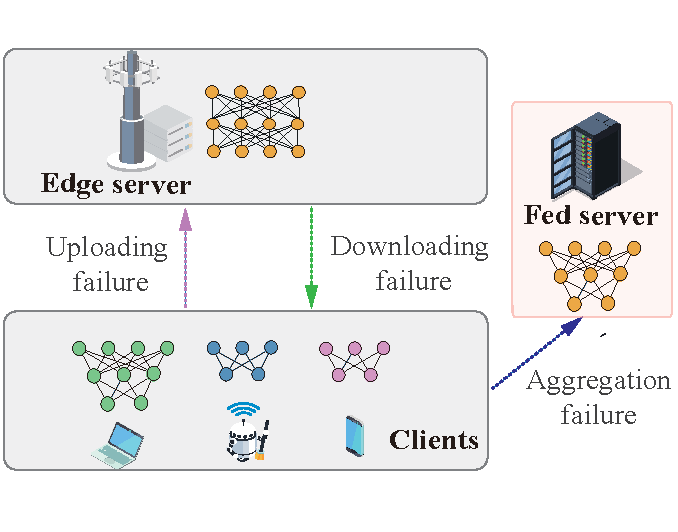
\includegraphics[width=4.1cm]{figures/illustration-pphia.pdf}
	}
         \subfigure[\centering Test accuracy v.s. the index of cut layer.] {
 \centering
		\centering\includegraphics[width=4.1cm]{figures/motivation_1_different_I.pdf}
        }
	\centering\caption{(a)  SFL scenario exists uploading, downloading and aggregation failures due to unstable client participation. (b) The failure occurs exclusively during uploading, downloading, or aggregation,  with a probability ranging from 0.2 to 0.6. The experiments select 5 clients out of 100 clients in each training epoch. The training process, consisting of 500 epochs, is conducted with ResNet-50 on the CIFAR-10 dataset under non-IID settings. } 
		\label{sfig:motivation_1_different_I}
\end{figure}



% \begin{figure}[t]
% \vspace{-.5ex}
% \setlength\abovecaptionskip{3pt}
% \centering
% \subfigure[The impact of model splitting.]{
%     % \includegraphics[height=2.3cm,width=4cm]{hetero_compute.eps}
% \includegraphics[width=8.5cm]{On_demand_scheduling/figures/motivation_1_different_I.pdf}
%     \label{sfig:motivation_1_different_I}
% }
% % \hspace{.1cm}
% % \subfigure[The impact of client sampling.]{
% %     \includegraphics[width=3.85cm]{On_demand_scheduling/figures/motivation_cs.pdf}
% %     \label{sfig:moti_1_accuracy_communication_overhead}
% % }
%     \caption{ The impact of model splitting and client sampling strategies on training performance in unstable environment. The figure presents the performance for test accuracy versus the number of epochs.
% Our experimental setting selects 5 clients out of a total pool with 100 clients in each training round. All experiments are conducted on  NVIDIA GeForce RTX 4090 
%  with ResNet-50 on the CIFAR-10 dataset under the non-IID setting. Moreover, the cut layer $L_c$ is set to 19.}
%     \label{fig:motivation_1}
%     \vspace{-2ex}
% \end{figure}


% However, SL's sequential training requires each client to wait for the previous one to finish its operations, struggling to handle an increasing number of clients or larger datasets without sacrificing the training time.  
% To address these issues, a natural progression is to explore split federated learning (SFL)~\cite{thapa2022splitfed,10234718}. 
% In SFL approach, the federated server (Fed server) periodically aggregates both server-side and client-side sub-models—mirroring the federated learning paradigm\cite{9084352,konevcny2016federated}—to synchronize the global model.

However, although tremendous efforts have been made on SFL in recent years, prior SFL schemes could perform poorly under unreliable communication networks. Specifically, SFL requires not only periodical client-side model aggregation but also frequent exchanges of activations and activations' gradients between clients and the edge server during every forward and backward pass~\cite{thapa2022splitfed,lin2025hasfl,9923620,lin2025hsplitlora}. In practice, device instability and network fluctuations, caused by memory overflow, client mobility, or deep channel fading, can easily cause updating/transmission failures in SFL. As shown in Fig.~\ref{sfig:motivation_1_different_I} (a), three major failure cases exist. (i) \textit{uploading failures} may occur when a client cannot complete the forward pass in time due to limited processing power or fails to upload activations promptly because of poor uplink channel conditions; (ii) \textit{downloading failures} arise when the downlink channel conditions from the edge server is too harsh to download activations' gradients timely; and (iii) \textit{aggregation failures} happen when a client experiences adverse uplink or downlink channel conditions when exchanging client-side models with the Fed server for aggregation. Each of these failure cases negatively affect the overall efficiency and model convergence in SFL.

Tackling unstable client participation requires rigorous convergence analysis of SFL with unstable client participation. 
The \textbf{main challenge} lies in the fact that failure can occur at different SFL stages, and these stages have \textit{varying impacts} on training performance. 
As shown in Fig.~\ref{sfig:motivation_1_different_I} (b), uploading failures prevent both server-side and client-side model updates in the affected iteration, which causes the most severe degradation. Downloading failures only halt client-side updates and lead to a smaller impact. Aggregation failures result in missing client-side models and have a moderate effect.
The combined impact of these different failure types has not been theoretically quantified in the literature. This interplay fundamentally distinguishes the convergence analysis and optimization framework for SFL from those of conventional FL systems~\cite{9060868,10292582,chen2024fedmeld,hu2024accelerating}. Moreover, while some recent SFL studies have examined various aspects to improve robustness of SFL via dynamic weight adjustments \cite{10095067} and packet loss resilience \cite{shiranthika2023splitfedresiliencepacketloss}, none of them has theoretically characterized the impact of unstable client participation on SFL and developed a unified optimization framework under unstable conditions.

To address the above challenges, in this paper, we develop an SFL framework considering unstable client participation. To mitigate the adverse effect, optimizing client sampling and model splitting is the key. (i) \textit{Client sampling} should strike an optimal diversity-stability trade-off by sampling clients to preserve data diversity while also prioritizing relatively stable clients under non-IID data distributions. (ii) \textit{Model splitting} can also be optimized, as it affects communication-computing latency and determines how significantly client-side update failures influence overall training performance. Towards this end, we \textit{first} perform the convergence analysis of SFL under stable client participation by considering an impact of split points and failures in different stages. \textit{Then}, we devise an optimal client sampling and model splitting strategy for the SFL framework based on the theoretical upper bound. The primary contributions are as follows:


%Although some recent SFL works have explored various methods to improve robustness over noisy channels via dynamic weight adjustments \cite{10095067} and packet loss resilience \cite{shiranthika2023splitfedresiliencepacketloss}, none have specifically tackled the challenges of SFL optimization under unstable conditions by considering the impact of unstable client participation.

%These combined effect of  cannot be answered by conventional FL works.


%Although strategies such as adaptive update aggregating frequency and optimal selection of cut layers can expedite model convergence during the training process, they do not  address issues arising from unstable environments \cite{lin2024adaptsfl}. 

%underscores that the effectiveness of SFL critically depends on the strategic splitting of the model and the selection of the client that considers the varied loss probabilities of the model at different communication stages.

% Thus, it becomes evident that the effectiveness of SFL relies on strategic model splitting and client selection by taking the probability of client model loss during different stages into consideration.


% This limitation becomes particularly pronounced when amounts of clients are connected to an edge server, leading to heightened competition for the scarce bandwidth resource and further exacerbating communication latency. 

% Considering that clients, edge server and Fed server have to regularly exchange information (e.g., activations, activations' gradients, client-side model and server-side model) to cooperatively finishing SFL training, in practice, unstable network environment presents significant challenges to SFL training tasks due to limited bandwidth, variable latency, and intermittent connectivity—common in wireless and mobile networks. 










% \textcolor{blue}{Under stable network conditions, SFL effectively achieves distributed parallel training while preserving data privacy through the collaborative design of model splitting and model aggregation, 
% % combining the benefits of distributed, parallel training with the computational division of split learning, 
% thereby enabling efficient  training across multiple clients while still utilizing server-side resources for intensive computations.}
% % SFL combines the distributed, parallel training benefits with the division of computation in split learning, enabling more efficient and scalable training across multiple edge devices while still utilizing cloud resources for heavy computations.

% \subsection{突出网络不稳定研究在SFL中的作用}
% However, in practice, network instability is a significant challenge to SFL training task due to factors such as limited bandwidth, variable latency, and intermittent connectivity—common in wireless and mobile networks where edge devices operate. 
% Thus, the efficacy of SFL training task depends not only on the strategic partitioning of computational tasks but also critically on the network stability of update transmissions and synchronization among edge devices, clients, and servers as shown in \textbf{figure}. 



% In practice, network instability is a significant challenge due to factors such as limited bandwidth, variable latency, and intermittent connectivity—common in wireless and mobile networks where edge devices operate. 


% In real-world conditions, network fluctuations can lead to inconsistencies in the upload of intermediate activations, delays in the delivery of gradients or updated parameters, and disruptions during the aggregation stage. Such instability may adversely affect the training process through delayed or incomplete updates—where network congestion or packet loss prevents timely delivery of activations or gradients, resulting in the server working with stale or partial data—and inconsistent synchronization, which causes devices to operate with heterogeneous parameter versions. Moreover, challenges during aggregation can diminish the overall quality of the global model, thereby impairing its generalization performance on unseen datasets. 


% \subsection{以前的解决方案突出理论指导和clientsampling的作用}





%Non-IID data distributions across different clients also harm overall training performance by introducing significant bias and variance in the local updates


% Existing literature investigates the impact of unstable environment on the SFL training process:
% Smart SplitFed learning \cite{10095067} 
% mitigates the adverse effects of noisy communication links on feature and gradient transmission in SFL and ensures robust convergence under severe noise conditions by introducing a dynamic averaging strategy that modulates client weights based on local loss statistics. 
% Similarly, robust frameworks for U-shaped medical image networks adopt dynamic weight correction techniques \cite{yang2022robustsplitfederatedlearning} to counteract model drift caused by disparate data distributions and heterogeneous computing resources, leading to a more stable aggregated model. 
% Moreover, approaches such as Dynamic Federated Split Learning \cite{10547401} leverage resource-aware model partitioning combined with clustering based on neural network layer similarities to optimize training efficiency, reduce energy consumption, and maintain high accuracy in challenging environments. 
% Moreover, Shiranthika et al. \cite{shiranthika2023splitfedresiliencepacketloss}  study the impact of model split points on the packet loss resilience
% of SFL.
% Li et al. \cite{li2024core} investigate spatio-temporal dependencies and dynamic trends for SFL-based traffic prediction between clients and the server. 
% By analyzing local feature extracted from global model, it minimizes data transmission and mitigates delay and network congestion.
% demonstrate through empirical studies that deeper model splitting and advanced parameter aggregation strategies can significantly enhance SFL's resilience to packet loss. Totally, these contributions underscore the potential of tailored instability solutions in split federated learning to bridge the gap between unstable and stable training scenarios.



\begin{itemize}
\item  We provide the first theoretical convergence analysis that reveals how model splitting and client sampling strategies impact training convergence in SFL with unstable client participation.


% Key findings indicate that lower client participation probability
%  leads to a higher sampling probability, which balances client heterogeneity and ensures sufficient participation of clients with abundant data, to meet convergence targets.
% Moreover, we also derive that shallow model splitting point enhances SFL's resilience to model loss.
 \item Based on the convergence bound, we formulate a joint optimization framework for client sampling and model splitting aimed at minimizing the upper bound of training loss. We derive an optimal polynomial-time solution for client sampling and model splitting in SFL.
  
  \item Extensive simulations demonstrate that our proposed solution achieves superior test accuracy compared with baselines.
\end{itemize}

The remainder is outlined as follows. Section~\ref{Rel_Work} reviews prior literature. Section~\ref{sec:systemModel} introduces the system model. We further provide the convergence analysis for the optimal client sampling and model splitting framework and present the problem formulation in Section~\ref{convergence_SFL}. Section~\ref{solu_appro} develops the optimal solution to this problem, and Section~\ref{simulations} presents the simulation results. Finally, in Section~\ref{conclusion}, we conclude our work.



% Split Learning (SL) presents an alternative through vertical model partitioning. The OpenSplit whitepaper \cite{opensplit2023} reports 79\% memory reduction on edge devices in smart factory deployments. Yet Cisco's 2024 Distributed AI Benchmark shows SL's sequential training pipeline increases latency by 42-67\% compared to parallel FL architectures \cite{cisco2024split}. This fundamental trade-off between computational efficiency and system scalability forms the critical research frontier in edge AI deployment. 

% Distributed learning paradigms, such as Federated Learning (FL) \cite{9084352,konevcny2016federated} and Split Learning (SL)~\cite{vepakomma2018split,lin2023split}, have been developed to tackle the challenge of limited computational resources.  
% Federated Learning (FL), standardized in IEEE P3652.1 whitepaper \cite{ieee2022fl}, demonstrates 94\% less data transmission compared to centralized learning in cross-hospital MRI analysis \cite{10.1145/3442381.3449782}. However, as revealed in Meta's FL deployment case study, FL requires 2.3× more local computation than centralized approaches for BERT-base fine-tuning \cite{meta2022flops}. 

%  However, while FL maintains data privacy by keeping data on-device, it requires the training of full-scale models locally, resulting in significant computational overhead and large-volume parameter exchanges during model aggregation. Similarly, SL reduces the local computational burden by splitting the model but often involves a sequential training process that can lead to increased latency and limited scalability.
 
% Split Federated Learning (SFL) is an emerging paradigm that integrates the advantages of federated learning and split learning to efficiently train large-scale models on edge devices while mitigating communication and privacy challenges.
% In SFL, the global model is partitioned into client-side and server-side sub-models, where edge devices perform local computations on raw data and transmit only intermediate activations and gradients to a powerful server for further processing. 
% This design allows edge devices to perform preliminary computations while offloading heavier processing to a centralized server, thereby reducing the burden on resource-limited clients.

\begin{table}[t]\label{notation}
\caption{{Summary of Important Notations.}}
{\small % 开始小字体区域
  \renewcommand{\arraystretch}{1.15}{
  \setlength{\tabcolsep}{0.1mm}{
\begin{tabular}{ll}
			\toprule
			\toprule
\textbf{Notation}                                                              & ~~~\textbf{Description}  \\ \hline
~~~$\mathcal{N}$ &  ~~~The set of all clients     \\
~~~$\mathcal{K}^{(t)}{(\bm q)}$ &  ~~~The set of clients randomly sampled in round 
$t$   \\
~~~$N$ &  ~~~The number of clients     \\
~~~$K$ &  ~~~The number of sampled clients     \\
~~~${\mathcal{D}_i}$           &  ~~~Client $i$'s local dataset  \\
~~~$f\left( {\bf{w}} \right)$     &  ~~~The global loss function parameterized by ${{\bf{w}}}$ \\
% ~~~$E$     &  ~~~The number of training epochs \\
~~~$R$     &  ~~~The number of training rounds \\
~~~${\mathcal{B}_i}$     &  ~~~The mini-batch sampled from ${\mathcal{D}_i}$ \\
~~~${b}$     &  ~~~The size of mini-batch \\
% ~~~$b$     &  ~~~The mini-batch size \\
~~~${{\bf{w}}_{c,i}}$/${{\bf{w}}_{s,i}}$            &  ~~~The client-side/server-side sub-model of client $i$  \\
~~~${\bf{ h}}_{s}$           &  ~~~The server-side common sub-model  \\
~~~${{\bf{ h}}_{m,i}}$           &  ~~~The server-side non-common sub-model of client $i$  \\
 ~~~${{\bf{h}}_{c,i}}$           &  ~~~The forged client-specific model of client $i$  \\
~~~$L_c$           &  ~~~The maximum cut layer index of all clients  \\
~~~$L$           &  ~~~The number of layers in the global model  \\
~~~$L_c^i$           &  ~~~The cut layer of client $i$   \\
% ~~~${{f _s}}$/${{f _i}}$           &  ~~~The computing capability of server/edge device $i$  \\
% ~~~${\rho _j}$/${\varpi _j}$           &  ~~~The FP/BP computing workload of propagating the\\
% & ~~ first $j$ layer neural  network for one data sample\\
% ~~~${\psi _j}$/${\chi _j}$           &  ~~~The data size of the activations/activations' gradients\\
% &  ~~ at the cut layer $j$\\
% ~~~${\delta _j}$           &  ~~ The data size of client-side sub-model with the cut layer $j$ \\
% ~~~${r_i^{U}}$/$r_{i,f}^U$       &  ~~~The uplink transmission rate from edge device $i$ to \\
% &  ~~ edge server/fed server.\\
% ~~~${r_i^{D}}$/$r_{i,f}^D$    &  ~~~The downlink transmission rate from edge server/ \\
% &  ~~ fed server to edge device $i$.\\
% ~~~$r_{s,f}$    &  ~~~The transmission rate from the edge server to fed  \\
% &  ~~ server. \\
% ~~~$r_{f,s}$    &  ~~~The transmission rate from fed server to edge server. \\
~~~$\beta, {\sigma _j^2}, {G _j^2}$     &  ~~ Loss function constants (detailed in Section~\ref{convergence_SFL})\\
~~~$I$           &  ~~~The interval (in iterations) between client-side MA
\\
~~~$p_i$           &  ~~~Upload failure probability from client $i$
 to server
\\
~~~$\varphi_i$           &  ~~~Download failure  probability  from  server to client $i$
\\
~~~$a_i$           &  ~~~Upload failure probability from client $i$
 to Fed server
\\
~~~$\bm q$           &  ~~~Client sampling probability
\\
~~~$m_i$           &  ~~~The weight of client i's dataset
\\
~~~${s_{u}^{i}}, {s_{d}^{i}}, {s_{a}^{i}}$           &  ~~~Bernoulli random variables
\\
~~~$\gamma$           &  ~~~Learning rate
% \\
% ~~~$T_1$-$T_6$           &  ~~~The auxiliary variables (to linearize problem~\eqref{problem_1})
\\ \bottomrule
\end{tabular}}}
}
\end{table}





\section{Related Work}\label{Rel_Work}
% \subsection{有没有工作分析过SFL/sl/fed中的不稳定的问题}
% \cite{yang2022robustsplitfederatedlearning}(sfl)
% \subsection{有没有工作分析过SFL/sl/fed中的client sampling问题}
% \cite{10547401}

\textbf{Convergence analysis of FL.}
FedAvg~\cite{mcmahan2017communication} is widely recognized as the first and the most commonly used FL algorithm. Several works have shown the convergence of FedAvg under different settings, e.g., IID setting~\cite{10.5555/3546258.3546471,NEURIPS2018_3ec27c2c}, non-IID setting~\cite{10292582,9261995} even with partial clients participation~\cite{cho2020clientselectionfederatedlearning}.
% Numerous studies in FL have conducted the convergence analysis\cite{10292582,9261995}.
% Unstable client participation presents a critical challenge in FL paradigms. 
% This instability is primarily driven by two factors: first, the communication environment’s instability caused by network congestion, bandwidth fluctuations, and signal attenuation; and second, the intentional dropout of clients for energy conservation or resource management purposes.
% Numerous studies in FL have addressed the unstable communication issue with various techniques, including local updating strategies \cite{9716792}, client sampling \cite{9491936},  sparsification \cite{10.1609/aaai.v37i7.25977}, and quantization\cite{10658402}.
% Soft-DSGD \cite{9716792} is a robust decentralized SGD algorithm that leverages partially received messages and adapts mixing weights based on communication link reliability to overcome the challenges of unstable communications in decentralized FL, while achieving the same asymptotic convergence rate as in perfectly reliable networks
Under IID conditions, Wang et al. \cite{10.5555/3546258.3546471} present a unified framework for communication‑efficient strategies and establish convergence guarantees that both reduce communication overhead and achieve fast error convergence. 
Moreover, Woodworth et al.~\cite{NEURIPS2018_3ec27c2c} introduce a graph‑based oracle model for parallel stochastic optimization and derive the optimal lower bound that depends only on the graph depth and size, thereby clarifying fundamental limits of communication–parallelism trade-offs.
For non-IID settings, Rodio et al.~\cite{10292582} analyze heterogeneous and temporally/spatially correlated client availability, demonstrating that correlation deteriorates FedAvg’s convergence rate if not handled properly.
Dinh et al.~\cite{ 9261995} propose FEDL under strong convexity and smoothness, establish linear convergence by controlling local inexactness and learning rate. They derive closed-form solutions jointly tuning FL hyperparameters to balance wall-clock convergence and device energy costs. Meanwhile, Cho et al. \cite{cho2020clientselectionfederatedlearning} study biased client selection under partial participation and show that prioritizing high-loss clients accelerates FedAvg’s convergence but may introduce a small bias tied to data heterogeneity.
% employ a finite-state Markov chain to analyze the spatiotemporal correlations in client availability, demonstrating that clients in the same time frame or geographical region tend to exhibit similar online and offline patterns, which in turn can slow down the convergence rates if not handled properly. 
% Besides, the work presented in \cite{9261995} analyzes the convergence of FL by enabling heterogeneous clients to update their local models with controlled accuracy. The system achieves a trade-off that is Pareto optimal among convergence speed, communication cost, and local computation accuracy.
% Unlike FL, SFL demonstrates significantly higher sensitivity to unstable client participation due to its continuous client-server communication requirements and high-dimensional data transmission volumes of intermediate representations \cite{10095067,shiranthika2023splitfedresiliencepacketloss}: 
% To overcome this issue, SFL in \cite{10095067} 
% mitigates the adverse effects of noisy communication links on feature and gradient transmission in SFL and ensures robust convergence under severe noise conditions by introducing a dynamic averaging strategy that modulates client weights based on local loss statistics. 
% Similarly, robust frameworks for U-shaped medical image networks adopt dynamic weight correction techniques \cite{yang2022robustsplitfederatedlearning} to counteract model drift caused by disparate data distributions and heterogeneous computing resources, leading to a more stable aggregated model. 
% Moreover, approaches such as Dynamic Federated Split Learning \cite{10547401} leverage resource-aware model partitioning combined with clustering based on neural network layer similarities to optimize training efficiency, reduce energy consumption, and maintain high accuracy in challenging environments. 
% Moreover, Shiranthika et al. \cite{shiranthika2023splitfedresiliencepacketloss}  study the impact of model split points on the packet loss resilience
% of SFL.
% \textcolor{blue}{Li et al. \cite{li2024core} investigate spatio-temporal dependencies and dynamic trends for SFL-based traffic prediction between clients and the server. By analyzing local feature extracted from global model, it minimizes data transmission and mitigates delay and network congestion.}
% demonstrate through empirical studies that deeper model splitting and advanced parameter aggregation strategies can significantly enhance SFL's resilience to packet loss. Totally, these contributions underscore the potential of tailored instability solutions in split federated learning to bridge the gap between unstable and stable training scenarios.
% However, none have provided convergence analysis nor tackled the challenges of strategic model splitting and dynamic client selection under unstable conditions. 
However, despite extensive convergence analyses in FL, existing FL convergence bounds do not directly apply to SFL due to architectural differences, as they often neglect SFL’s frequent communications and the impact of model splitting on convergence.


%Thus, a comprehensive theoretical framework for understanding the impact of insatiability on overall SFL training performance remains an open issue.

\textbf{Client sampling.} Client sampling is a critical design component in distributed machine learning across heterogeneous devices. In the existing FL literature, client sampling strategies primarily include uniform sampling \cite{mcmahan2017communication}, importance-aware sampling~\cite{chen2022optimalclientsamplingfederated,9904868,pmlr-v151-jee-cho22a}, clustering-based sampling~\cite{fraboni2021clustered,NEURIPS2024_7886b9ba}, resource-aware sampling \cite{10.1109/INFOCOM48880.2022.9796935}, and fairness-aware sampling \cite{9810502}. Uniform sampling refers to randomly selecting a fixed proportion of clients from the total pool during each training round. Despite its simplicity, uniform sampling does not account for system or data heterogeneity. Importance sampling mitigates the high variance inherent in stochastic optimization methods like stochastic gradient descent (SGD) by preferentially sampling clients with more ``important'' data. Specifically, these approaches assign higher sampling probabilities to clients whose contributions are quantified using local gradients (e.g., \cite{chen2022optimalclientsamplingfederated,9904868}) or local losses (e.g., \cite{pmlr-v151-jee-cho22a}). 
% \textcolor{blue}{On the other hand, resource-aware optimization-based methods address system-level challenges by focusing on the efficient allocation of resources. These approaches target issues such as CPU frequency allocation (e.g., \cite{8737464}), communication bandwidth distribution (e.g., \cite{9292468,9563947}), straggler-aware client scheduling (e.g., \cite{9355774,9563062}), parameter control (e.g., \cite{8664630}), and task offloading (e.g., \cite{9437529}).} 
Clustering-based sampling first groups clients according to the similarity of their data features or model updates and then selects representative clients from each group~\cite{fraboni2021clustered,NEURIPS2024_7886b9ba}. Resource-aware sampling takes into account the available system resources, such as communication and computational resources, when choosing participating clients  for each training round~\cite{10.1109/INFOCOM48880.2022.9796935,9810502}.  However, the above methods are tailored for traditional FL, which is inapplicable to SFL because SFL has different training stages as alluded earlier.

%Fraboni et al. \cite{fraboni2021clustered} demonstrate that by clustering clients prior to sampling, one can significantly reduce the variance in aggregated updates and improve overall convergence by ensuring that even clients with less ``important'' but unique data are appropriately represented in the global model. HiCS-FL \cite{NEURIPS2024_7886b9ba}, a hierarchical clustered sampling method for non-IID FL, uses output layer updates to estimate client data heterogeneity via an entropy-like measure, and then clusters clients and preferentially selects those with more balanced data, leading to faster convergence and improved model performance with minimal extra overhead.

%For instance, Luo et al.~\cite{10.1109/INFOCOM48880.2022.9796935} derive a convergence bound for resource-aware client sampling, formulate a non-convex optimization problem, and propose an adaptive sampling algorithm that minimizes wall-clock time. Fairness-aware sampling (e.g., Eiffel \cite{9810502}) ensures that clients with different data distributions or lower participation frequencies are adequately represented in the global model update via considering local model loss, data size, computation power, resource demand, and even the age of the last update.


% \textcolor{blue}{The server aggregates every round, while clients perform full local aggregations only every few rounds, resulting in asynchronous updates, which leads to stale information and complicates the accurate measurement of client contributions, ultimately affecting the global model's convergence behavior.
% Moreover, SFL clients can encounter failures in activations uploading, gradient downloading, and model aggregation.}

\textbf{Model splitting.} Model splitting plays a critical role in SFL, especially in scenarios with unstable client participation. The selection of the split point influences both communication/computation latency and overall training performance~\cite{ZW2024ultra-LoLa,zw2025AIoutage}. Several studies have investigated how to determine the optimal model splitting point for SFL \cite{lin2024adaptsfl,10980018,10304624,shiranthika2023splitfedresiliencepacketloss}. 
Shiranthika et al. \cite{shiranthika2023splitfedresiliencepacketloss}  study the impact of model splitting strategies on the packet loss resilience
of SFL. 
Lin et al. \cite{lin2024adaptsfl,10980018} investigate how the model splitting point affects training convergence, revealing that a shallower split point leads to smaller convergence upper bound. Xu et al. \cite{10304624} propose a combined optimization approach to identify the best split point and bandwidth allocation, aiming to reduce total training latency. Unfortunately, these studies overlook how model splitting affects training convergence with unstable client participation. To the best of our knowledge, our research is the first to analyze convergence of SFL under unstable client participation and explore client sampling and model splitting under the context of SFL. 

% We propose a novel client sampling strategy that leverages rigorous convergence analysis to guide its design, ensuring more effective global model convergence even under unstable condition.





% \subsection{有没有工作分析过SFL/sl/fed中的client sampling/unstble/且有理论指导问题}

\section{%
Preliminaries and System Model}
\label{sec:systemModel}





\begin{figure*}[t!]
\centering
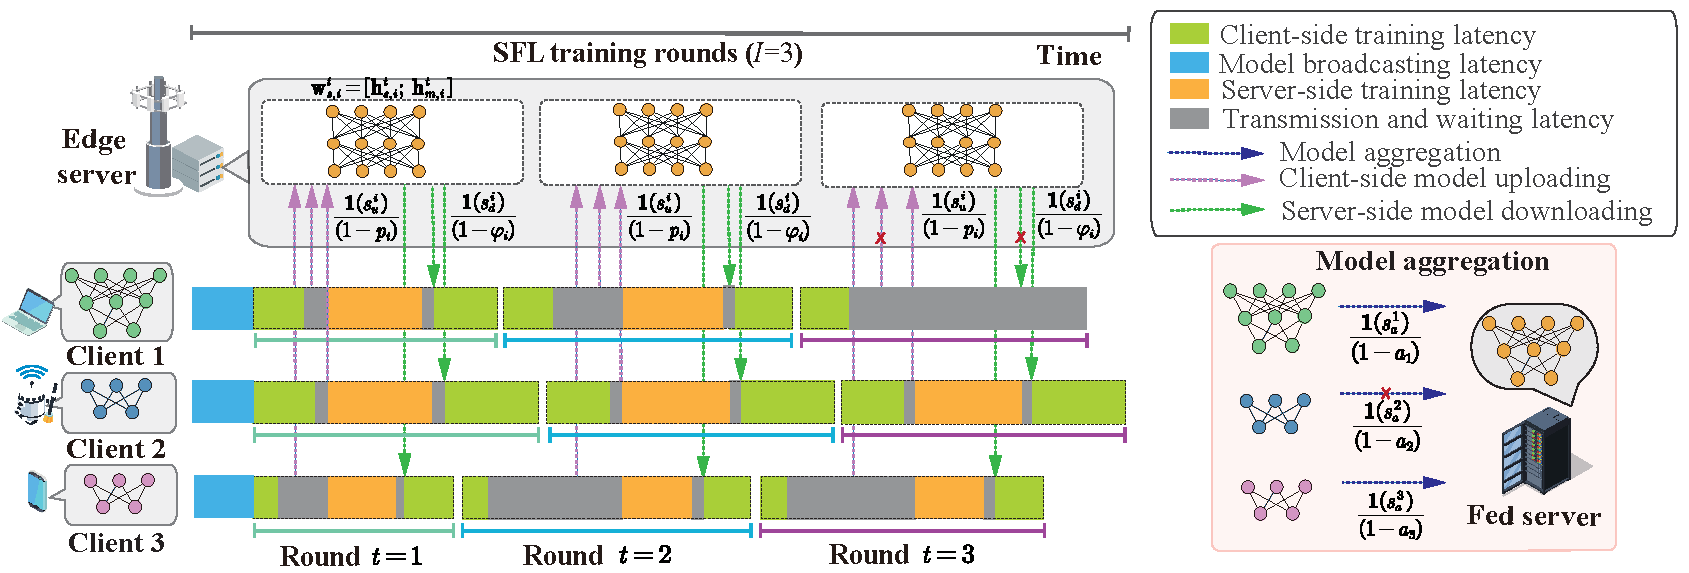
\includegraphics[width=16.5cm]{figures/unstable_0818.pdf}
\caption{Split federated
learning with unstable clients.  The main challenge for tackling unstable client participation lies in that failure can occur at different SFL stages, including activation uploading, gradient downloading, and client-side model aggregation, which have varying impacts on training performance.  $
p_i
$
is the probability that  client $i$'s upload to the edge server fails. $\varphi_i$ represents the probability that client $i$ experiences a downlink failure from the edge server. $a_i$ is the probability that client $i$'s upload to the Fed server fails. }
\label{multi-system}
\end{figure*}
\subsection{Typical SFL Framework}%
We study an SFL framework with an edge server coordinating a client set $\mathcal{N} = \{1, \ldots, N\}$, where $N$ denotes the total number of clients. The overall process is described in detail as follows:
\begin{itemize}
\item \textbf{Client side}:  Each client $i$ possesses $D_i$ local training samples, where \(\mathbf{x}_{i,k}\) indicates the input data of the \(k-\)th sample and \(y_{i,k}\) represents its corresponding label, forming the dataset $\mathcal{D}_i=\{( \mathbf{x}_{i, k},y_{i, k})\}_{k=1}^{D_i}$. Across all 
$N$ clients, the total number of training samples is $D :=\sum\nolimits_{i = 1}^N D_i$. 
Moreover, ${{\bf{w}}_{c,i}}$ denotes the client-side sub-model of client $i$. 
\item \textbf{Edge server}: The edge server acts as a high-performance central computing node that performs training on server-side sub-models. For client $i$, the server-side sub-model is represented as  ${{\bf{w}}_{s,i}} = \left[{{\bf{h}}_{s}};{{\bf{h}}_{m,i}}\right]$, where ${\bf{h}}_{s}$ is the common component shared across all clients and synchronized in every round. Moreover, ${\bf{h}}_{m,i}$ is the non-common (personalized) portion, which is specific to clients with additional layers on the server and is aggregated every 
$I$ rounds. Additionally, the edge server gathers key network information, including client's computing capabilities and channel conditions, to facilitate optimized decision-making.
\item \textbf{Fed server}: 
The Fed server coordinates and synchronizes client-side sub-models by aggregating these sub-models at regular intervals from participating clients.
To address privacy risks, the Fed server and edge server are typically operated by different entities~\cite{10.1145/3460120.3485259}. 
\end{itemize}

% Further,  ${{f}\left( \mathbf{w}; \mathbf{x}_{i, j} \right)}$ indicates how the machine learning model parameter $\mathbf{w}$ performs on the input data sample $\mathbf{x}_{i, j}$. Thus, the local loss function of client $i$ can be defined as 
% \begin{equation}
% \label{lo_ob}
% {F_i}\left( \mathbf{w} \right) := \frac{1}{{{n_i}}}\sum\nolimits_{j =1}^{n_i} {{f}\left( \mathbf{w}; \mathbf{x}_{i, j} \right)}.
% \end{equation}
% Denote $p_i=\frac{n_i}{n_\textnormal{tot}}$ as the weight of the $i$-th device such that $\sum\nolimits_{i = 1}^N p_i=1$. Then, by denoting $F\left( \mathbf{w} \right)$ as the global loss function, the goal of FL is to solve the following optimization problem 
% \cite{kairouz2019advances}:
% \begin{equation}
% \label{gl_ob}
% \min_{\mathbf{w}}  F\left( \mathbf{w} \right) :=\sum\nolimits_{i = 1}^N{p_i}{F_i}\left( \mathbf{w} \right).
% \end{equation}


\subsubsection{Global Model and Objective}
The global model isdenoted as ${\bf{w}} = \left[ {{{\bf{w}}_{s,i}};{{\bf{w}}_{c,i}}} \right] $, where ${{\bf{w}}_{s,i}}$ represents server-side sub-model and ${{\bf{w}}_{c,i}}$ represents client-side submodel of client $i$, respectively. The objective of SFL is to minimize the global training loss
\begin{align}\label{minimiaze_loss_function}
\mathop {\min }\limits_{\bf{w}} f\left( {\bf{w}} \right) \buildrel \Delta \over = \mathop {\min }\limits_{\bf{w}} {\frac{{{1}}}{N}} \sum\limits_{i = 1}^N {f_i}({\bf{w}}),
\end{align}
where ${f_i}\left( {\bf{w}} \right) \buildrel \Delta \over = {\mathbb{E}_{{\xi _i} \sim {\mathcal{D}_i}}}[{F_i}\left( {{\bf{w}};{\xi _i}} \right)]$ is client $i$'s local loss function, and $\xi _i$ represents stochastic mini-batch sampling from dataset $\mathcal{D}_i$. Moreover, the stochastic gradient $\nabla F_{i}(\mathbf{w}^{t};\xi_{i}^{t}) $ is an unbiased estimate of $\nabla f_{i}(\mathbf{w})$ with $\mathbb{E}_{\xi_{i}^{t}\sim \mathcal{D}_{i}}[\nabla_{\bf{w}} F_{i}(\mathbf{w}^{t-1}_{i};\xi_{i}^{t}) \vert \boldsymbol{\xi}^{[t-1]}] = \nabla f_{i}(\mathbf{w}^{t-1}_{i})$, where $\boldsymbol{\xi}^{[t-1]}$ encompasses all randomness up to round $t-1$, defined as $\boldsymbol{\xi}^{[t-1]} \overset{\Delta}{=} [\xi_{i}^{\tau}]_{i\in\{1,2,\ldots,N\}, \tau\in\{1,\ldots,t-1\}}$~\cite{pmlr-v119-karimireddy20a}. Besides, {${\nabla _{\bf{w}}}F({\bf{w}}; \xi)$ denotes the first-order derivative (gradient) of $F({\bf{w}}; \xi)$ with respect to the parameter vector ${\bf{w}}$.}


\subsubsection{{Client Sampling}}%
We sample clients based on a probability distribution
\begin{align}
\boldsymbol{q} = \{q_i\}_{i\in\mathcal{N}}, 
\quad 0 \le q_i \le 1,
\end{align}
with the constraint $\sum_{i=1}^Nq_i\!=\!1$. By optimizing $\boldsymbol{q}$, we jointly account for system‐level heterogeneity (e.g., unstable communication status) and statistical heterogeneity (non‐i.i.d. data distributions across clients) in order to minimize the global training loss for convergence. 
% The specific client sampling model is as follows.
% We consider a standard SFL setting where the training data are distributed in an unbalanced and  non-i.i.d. fashion among clients. 
Following recent works 
\cite{li2019convergence,yang2021achieving}, we assume that, at each round \(t\), the server samples clients from  client set $  \mathcal{N}$, performing $K$ times with replacement based on the probability \(\boldsymbol{q}\). The resulting client set is denoted as $\mathcal{K}^{(t)}(\boldsymbol{q})$, where $\mathcal{K}^{(t)}\! \subseteq\!  \mathcal{N}$ and $K\! :=\! \left| \mathcal{K}^{(t)}\right|$. 
% Notably, we assume that during each  $I$ training rounds between two consecutive client-side model aggregation, the client sampling set is unchanged and thus there exists $r=\lceil t/I \rceil$.
% In this scenario, a client may appear multiple times in $\mathcal{K}^{(t)}(\boldsymbol{q})$. The aggregation weight for each client $i$ corresponds to the frequency of its appearance in $\mathcal{K}^{(t)}(\boldsymbol{q})$.
Since sampling is with replacement, a given client \(i\) may appear multiple times in \(\mathcal{K}^{(t)}\).  In the subsequent aggregation step, the aggregation weight for each client proportions to the number of its appearances in $\mathcal{K}^{(t)}(\boldsymbol{q})$.


\subsubsection{Training Process}
Before training, the edge server initializes the machine learning model, splits it into client-side and server-side sub-models, distribute these sub-models to clients and edge server, and determines the optimal client sampling strategy. Afterwards, SFL training process is executed in $I$ rounds, repeating until convergence.
The workflow comprises two phases: \textit{split training} and \textit{client-side model aggregation}.  Split training occurs every round, while the model aggregation of clients is performed every $I$ rounds. Specifically, for  round $t \in \mathcal{R} = \left\{ {1,2,...,R} \right\}$, the SFL framework proceeds as follows.

% Here, denoting $r$ as the index of the number of communication rounds, %
% we  describe one round (e.g., the $r$-th) of the workflow of SFL framework as follows: 

\textit{a. Split Training Stage:} Executed in each training round, this stage updates sub-models of the participating clients and the edge server, and is composed of three sequential steps:



\textit{a1) Client-side Model Forward Pass and Activations' Transmission:} In this step, the selected clients execute client-side forward pass (FP) simultaneously. To be specific, client $i$ samples a mini-batch ${\mathcal{B}_i}$ of batch size
$b $ from the local dataset ${\mathcal{D}_i}$, 
% The input data and corresponding label of mini-batch in training round $t$ are denoted by ${{\bf{x}}^t_i}$ and ${{\bf{y}}^t_i}$,
% ${\bf{w}}^{t-1}_{c,i}$ represents the client-side sub-model of client $i$.
feeds it through the corresponding client-side sub-model to generate activations at the cut layer, and then transmits these activations along with the labels to the edge server, typically via wireless channels. The edge server then uses the received activations to update the server-side sub-model.

% Moreover, each client’s per‐round latency $T_i^{U}$ during model forward pass and activations' transmission is composed of its computation latency $\tau _{i}^{c}(L_{c}^{ i })$ and its upload time $t_{i}^{\mathrm{up}}(L_{c}^{ i })$, which is expressed by:
% \begin{equation}\label{eq:latency}
% T_i^{U} \;=\tau _{i}^{c}(L_{c}^{ i }) +  t_{i}^{U}(L_{c}^{ i }),
% \end{equation}
% where
% \begin{equation}
%  t_{i}^{U}(L_{c}^{ i })=\frac{S_A\bigl(L_c^i\bigr)}{r_i^U}\,, 
% \end{equation}
%  and $S_A(L_c^i)$ is the total size of activations generated by the client-side model at cut layer $L_c^i$.
%   By the central‐limit theorem \cite{dudley1978central}, we model the uplink rate as
% $r_i^U \sim \mathcal{N}(\mu_i^U,{\sigma_i^U}^2)$
% so as to compactly capture the aggregate impact of multiple, independently varying channel impairments (path‐loss, shadowing, interference, etc.).
% Specifically, $\mu_i^U$ is the mean of uplink rate, capturing average wireless throughput (path loss, shadowing, network load) and ${\sigma_i^U}^2$ is its variance, measuring rate fluctuations \cite{johnson2004information}.

% \textcolor{blue}{With above definitions, we further declare an upload failure whenever $T_i^U > T_{\max}^U$, which is denoted by
% \begin{align}\label{eq:failure_prob}
% p_i(L_{c}^{ i })
% &= \Pr\bigl[T_i^U > T_{\max}^U\bigr] 
% = \Pr\!\Bigl[r_i^U < \frac{S_A(L_c^i)}{T_{\max}^U-\tau _{i}^{c}}\Bigr] \notag
% \\&= \Phi\!\Bigl(\frac{\,S_A(L_c^i)/(T_{\max}^U-\tau _{i}^{c}(L_{c}^{ i }))-\mu_i^U\,}{\sigma_i^U}\Bigr)\,,
% \end{align}
% where $\Pr[\cdot]$ denotes the probability of an event and $\Phi(\cdot)$ is the standard Gaussian  cumulative distribution function (CDF). } 


\textit{a2) Server-side Model Forward Pass and Backward Pass:} The edge server receives the activations and feeds them into the respective server-side sub-models. Specifically, for client $i$, the prediction is given by
\begin{align}\label{stage_1_3}
{\bf{\hat y}}^t_i = \eta  \left( {{\bf{a}}^t_i;{{\bf{w}}^{t-1}_{s,i}}} \right),
\end{align}
where ${{\bf{w}}^{t-1}_{s,i}} = \left[{{\bf{ h}}^{t-1}_{s}};{{\bf{ h}}^{t-1}_{m,i}}\right]$. Here,
${\bf{ h}}^{t-1}_{s}$ represent the server-side common sub-model, while ${\bf{h}}^{t-1}_{m,i}$ refers to server-side non-common sub-model. 
% The predicted value and labels are utilized to calculate loss function value and further derive the server-side sub-model's gradients.
% \begin{align}\label{stage_5_2}
% {\bf{g}}_{s,i}^t = \left[ {{\nabla _{{{\bf{h}}_s}}}{F_i}({\bf{h}}_s^{t - 1};\xi _i^t);{\nabla _{{{\bf{h}}_m}}}{F_i}({\bf{h}}_{m,i}^{t - 1};\xi _i^t)} \right],
% \end{align}
Specifically, the edge server updates $\mathbf{h}_{s}^{t}$ as follows
\begin{align}\label{stage_5_2}
\mathbf{h}_{s}^{t}=\frac{1}{K}\sum_{i\in \mathcal{K} ^{(t)}(\boldsymbol{q})}{\frac{m_i}{q_i}}\mathbf{h}_{s,i}^{t},
\end{align}
where $m_i$ represents client $i$'s dataset weight. Moreover,  $\mathbf{h}_{s,i}^{t}$ denotes the server-side common sub-model  of client $i$, which is detailed by
\begin{align}
\,\,\mathbf{h}_{s,i}^{t}\gets \mathbf{h}_{s,i}^{t-1}-\gamma \frac{\mathbf{1}\!\left( {s_{u}^{i}} \right)}{\left( 1-p_i \right)}\nabla _{\mathbf{h}_s}F_i(\mathbf{h}_{s,i}^{t-1};\xi _{i}^{t}),
\end{align}
where $\gamma$ denotes the learning rate and $\nabla _{\mathbf{h}_s}F_i(\mathbf{h}_{s,i}^{t-1};\xi _{i}^{t})$ represents the stochastic gradient.  
Here, ${s_{u}^{i}}$ is the Bernoulli random variable that indicates whether the sub-model upload of the client $i$ to the server is successful \cite{10121038}.
Specifically,
$
{s_{u}^{i}} \sim \mathrm{Bernoulli}(1 - p_i),
$
where 
$
p_i
$
is the probability that  client $i$'s upload to the edge server fails.
Moreover, the indicator function expressed by
\begin{align}
&\mathbf{1}\!\left( {s_{u}^{i}} \right) =\left\{ \begin{array}{l}
	1,\ \text{with}\ \text{probability}\ 1-p_i,\\
	0,\ \text{with}\ \text{probability}\ p_i,\\
\end{array} \right. 
\end{align}
ensures that only the updates from clients whose uploads have actually succeeded are included in the subsequent server-side aggregation, while dividing by \(1-p_i\) keeps the estimator unbiased in expectation despite random upload failures.
The server-side non-common sub-model $\mathbf{h}_{m,i}^{t}$ is dictated by the heterogeneous cut layers: 
clients that offload more layers to the server induce personalized parts of server-side sub-models. Moreover, the updating rule for each client \(i\) updates its own non‐common sub‐model is
\begin{align}\label{non_commen_update}
\mathbf{h}_{m,i}^{t}\gets \mathbf{h}_{m,i}^{t-1}-\gamma \frac{\mathbf{1}\!\left( {s_{u}^{i}} \right)}{\left( 1-p_i \right)}\nabla _{\mathbf{h}_m}F_i(\mathbf{h}_{m,i}^{t-1};\xi _{i}^{t}),
\end{align}
where  ${\nabla _{{{\bf{h}}_m}}}{F_i}({\bf{h}}_{m,i}^{t - 1};\xi _i^t)$ represents the stochastic gradient. 

% Moreover, each client’s per‐round latency $T_i^{U}$ during model forward pass and activations' transmission is composed of its computation latency $\tau _{i}^{c}(L_{c}^{ i })$ and its upload time $t_{i}^{\mathrm{up}}(L_{c}^{ i })$, which is expressed by:
% \begin{equation}
% T_i^D
% = \tau_i^s\bigl(L_c^i\bigr)
% + t_i^D\bigl(L_c^i\bigr)
% \,,
% \end{equation}
% where
% \begin{equation}
% t_i^D\bigl(L_c^i\bigr)
% = \frac{S_{ G}\bigl(L_c^i\bigr)}{r_i^D}\,.
% \end{equation}
% Here,
% $
% r_i^D \sim \mathcal{N}\bigl(\mu_i^D,\,(\sigma_i^D)^2\bigr)
% $
% denotes the downlink rate and \(S_{G}(L_c^i)\) is the total size of the gradients transmitted from the server-side model to client-side model. Moreover, \(\tau_i^s(L_c^i)\) is the server-side computation time for layers above \(L_c^i\), including FP and BP process.  
% \textcolor{blue}{With above definitions, 
% we define a downlink failure happens when \(T_i^D > T_{\max}^D\), so
% \begin{align}
% \varphi_i(L_{c}^{ i })
% &= \Pr\bigl[T_i^D > T_{\max}^D\bigr]
% = \Pr\!\Bigl[r_i^D < \frac{S_{G}(L_c^i)}{T_{\max}^D - \tau_i^s(L_c^i)}\Bigr] \notag\\
% &= \Phi\!\Bigl(\frac{\,S_{G}(L_c^i)/(T_{\max}^D - \tau_i^s(L_c^i)) - \mu_i^D\,}{\sigma_i^D}\Bigr).
% \end{align}
% }

\textit{a3) Activations' Gradients Transmissions and Client-side Model Backward Pass:} After the server‐side backward pass finishing, the edge server transmits gradients back to each client. Upon receiving these gradients, each client updates its client‐side sub‐model. For client \(i\), the update rule is
\begin{align}\label{client_side_update}
\mathbf{w}_{c,i}^{t}\gets \mathbf{w}_{c,i}^{t-1}-\gamma \frac{\mathbf{1}\!\left( {s_{u}^{i}},\,\,{s_{d}^{i}} \right)}{\left( 1-p_i \right) \left( 1-\varphi _i \right)}\nabla _{\mathbf{w}_c}F_i(\mathbf{w}_{c,i}^{t-1};\xi _{i}^{t}),
\end{align}
where $
{s_{u}^{i}} \sim \mathrm{Bernoulli}(1 - p_i)$ and 
${s_{d}^{i}} \sim \mathrm{Bernoulli}(1 - \varphi_i)
$.
Moreover, 
$\varphi_i$ represents the probability that client $i$ experiences a downlink failure from the edge server. 
% Moreover, 
% \(p_i\) represents the probability that client \(i\)’s submodel upload fails,
% and \(\varphi_i\) is the probability that the downloaded activation gradients fail to arrive.
The combined indicator
% \begin{align*}
% &\mathbf{1}\!\left( {s_{u}^{i}},\ {s_{d}^{i}} \right) =\left\{ \begin{array}{l}
% 	1,\ \text{with}\ \text{probablity}\ (1-p_i)(1-\varphi _i),\\
% 	0,\ \text{with}\ \text{probablity}\ 1- (1-p_i)(1-\varphi _i).\\
% \end{array} \right. 
% \end{align*}
satisfies
\begin{align}
\Pr\{\,\mathbf{1}({s_{u}^{i}},{s_{d}^{i}})=1\} \;=\;(1-p_i)\,(1-\varphi_i).
\end{align}
Similarly, the indicator function in Eq.~\eqref{client_side_update} divided by \((1-p_i)(1-\varphi_i)\) ensures that the estimator remains unbiased in expectation despite possible communication failures.




% Similarly, the notation 
% $\mathbf{1}\!\left( {s_{u}^{i}},\ {s_{d}^{i}} \right)$ denotes an indicator function that returns $1$ if both of the following conditions are met: (1) client $i$'s submodel has been successfully uploaded to the server, and (2) the gradients have been successfully downloaded to the corresponding client $i$. Otherwise, it returns 
% 0. Specifically, the function is defined as follows
% \begin{align*}
% &\mathbf{1}\!\left( {s_{u}^{i}},\ {s_{d}^{i}} \right) =\left\{ \begin{array}{l}
% 	1,\ \text{with}\ \text{probablity}\ (1-p_i)(1-\varphi _i),\\
% 	0,\ \text{with}\ \text{probablity}\ 1- (1-p_i)(1-\varphi _i).\\
% \end{array} \right. 
% \end{align*}



\textit{b. Client-side Model Aggregation Stage:}  gathers and aggregates the client-specific models at the Fed server.
Each client-specific model consists of $\mathbf{h}_{m,i}^{t}$ and $\mathbf{w}_{c,i}^{t} $, aggregates every $I$ training rounds. The stage proceeds in three steps:

  \textit{b1) Model Upload:}
    Each client \(i\) sends its updated client‐side sub‐model \(\mathbf{w}_{c,i}^t\) and \(\mathbf{h}_{m,i}^t\) to the Fed server over the wireless/wired link.  Given the highly reliable inter-server link between edge server and the Fed server with sufficient bandwidth, we focus  on the upload failure of \(\mathbf{w}_{c,i}^t\) from clients to the Fed server in our analysis, and $a_i$ is the probability that client $i$'s upload to the Fed server fails.
%     Thus, the transmission time of the $i$-th client‐side submodel to the federated server for further aggragating is denoted by
% \begin{align}
%   t_{i}^{A} (L_c^i)
%   &= \frac{S_{J}(L_c^i)}{r_i^A}, 
% \end{align}
% where $S_{J}\bigl(L_c^i)$ is the size of client-side model and the data rate $r_i^A$ satisfies
% $ r_i^A \sim \mathcal{N}\bigl(\mu_i^A,\,(\sigma_i^A)^2\bigr)$. \textcolor{blue}{With above definitions, 
% We define an uploading failure with
%     \begin{equation}
%   a_i(L_c^i) \;=\;
%   \Pr\bigl[t_{i}^{A} (L_c^i) > T_{\max}^A\bigr]
%   \;=\;
%   1 - \Phi\!\Bigl(\frac{T_{\max}^A - \mu_i^A}{\sigma_i^A}\Bigr).
% \end{equation}


  \textit{b2) Client‐Side Model Aggregation:}
    Upon receipt of ${{\bf{h}}^t_{m,i}}$ and ${{\bf{ w}}^t_{c,i}}$, the server ``forges" each client’s full model by concatenating its server‐side and client‐side parts:
\begin{align}
    {{\bf{h}}^t_{c,i}} = \left[{{\bf{h}}^t_{m,i}};
\frac{\mathbf{1}\!\left( {s_{a}^{i}} \right)}{\left( 1-a_i \right)}
{{\bf{ w}}^t_{c,i}}\right],
    \end{align}
    where ${s_{a}^{i}} \sim \mathrm{Bernoulli}(1 - a_i)$. Here, \(\mathbf{1}({s_{a}^{i}})=1\) if the assembly succeeds (with probability \(1-a_i\)), and \(0\) otherwise.  
    The Fed server then aggregates these forged models as
    \begin{align}\label{h_c_define_refined}
      \mathbf{h}_{c}^{t}
      \;=\;
      \frac{1}{K}
      \sum_{i\in\mathcal{K}^{(t)}(\boldsymbol{q})}
      \frac{m_i}{q_i}\,
      \mathbf{h}_{c,i}^t,
    \end{align}
    where \(\mathcal{K}^{(t)}(\boldsymbol{q})\) refers to the set of \(K\) clients sampled with replacement according to \(\boldsymbol{q}\).

      \textit{b3) Model Download:} 
    Finally, the updated client-side sub-models are delivered to the corresponding clients, and the updated server-side non-common sub-models are deployed on the edge server, respectively.






% \textcolor{blue}{
% The above process repeats for many rounds until the global loss converges. 
% Recent works have demonstrated the effectiveness of split federated learning with theoretical convergence guarantees  in various settings 
% % \cite{
% % li2019convergence,haddadpour2019convergence,karimireddy2019scaffold,yang2021achieving, qu2020federated}
% . However, these works 
% assume that the server samples  clients either uniformly at random or proportional to data size, %
% which  may slow down the  wall-clock time for convergence %
% due to the straggling effect {e.g., clients’  non-i.i.d. data and diverse computational and communication capabilities}. %
%  Thus, a careful client sampling design should tackle both system and statistical heterogeneity for fast convergence.
%  }

This process is repeated until the global training loss converges. Although recent studies have established convergence guarantees for FL with client sampling \cite{li2019convergence,yang2021achieving}, they typically adopt uniform or data‐size‐proportional client sampling. 
Likewise, convergence analyses for SFL \cite{lin2024adaptsfl,han2025convergenceanalysissplitfederated} assume idealized conditions, such as stable network links and consistently available clients, conditions that rarely hold in realistic deployments.
 When deployed in unstable environments—characterized by fluctuating network links' conditions, intermittent client availability, and heterogeneous resources—these sampling strategies aggravate straggler delays, thereby prolonging total convergence time, and amplify oscillations in the aggregated model, resulting in degraded training accuracy.
  Thus, an optimal client sampling strategy that jointly accounts for unstable client participation and statistical heterogeneity is crucial for maintaining high accuracy while keeping the total training delay within acceptable bounds.




% \begin{figure}[t!]
% \centering
% \includegraphics[width=9cm]{unstable.pdf}
% 	\flushleft
% \caption{Adaptive heterogeneous client sampling for split
% federated learning.}
% \label{multi-system}
% \vspace{-1.5em}%%%%%%%%%%%%%%%%%%%%缩减竖直距离%%%%%%%%%%%%%%%%%%%%%%
% \end{figure}



% \subsubsection{System Heterogeneity Model}
% As illustrated in Fig.~1,  due to system bandwidth limitation and wireless interference, we assume that the sampled clients are scheduled in a frequency-sharing manner,   
% and each particular client's  com{p}utation time  for local model updates is static throughout the learning period as 
% % \cite{shi2020device, chen2020convergence,yang2020energy}. %
% %  \emph{Nevertheless, %
% % each client's  communication time  for model uploading varies across rounds, as the communication time depends on the allocated bandwidth in each round}.
% % \footnote{We do not consider the server's downlink time for model broadcasting and model aggregation, as we mainly focus on the performance bottleneck of the  battery-constrained edge devices.} %
% For example, the server may allocate different bandwidth for the same client in different rounds due to the randomly changing  sampled client set. 



% {\subsubsection{Joint Computation and Communication Design} 
% We consider the mainstream synchronized\footnote{As suggested \cite{bonawitz2016practical,avent2017blender,konevcny2016federated}, we consider mainstream synchronized SFL in this paper %
% due to its composability with other
% techniques (such as secure aggregation protocols and differential privacy).} SFL framework (e.g., \cite{mcmahan2017communication, bonawitz2019towards,   
% li2019convergence,haddadpour2019convergence,karimireddy2019scaffold,yang2021achieving, qu2020federated}), where the server waits to collect and aggregate all  sampled clients' model updates  before  entering the next round. For  SFL operating in the synchronized fashion,  the per-round time is limited by the slowest client (known as straggler).  
% % \emph{We can prove that for any sampling probability  $\boldsymbol{q}$, we will obtain a minimum round time $T^{(r)}(\boldsymbol{q})$ when the sampled $K$ clients complete their local model computation and model transmission at the same time.
% \footnote{Otherwise, simply allocating a certain amount of bandwidth from the earlier completed client to the straggler would yield a shorter round time.}} 
% In this way, consider sampled client $i$ at round $t \in [\lfloor t/I \rfloor,\lceil t/I \rceil]$, i.e., $i \in \mathcal{K}^{(r)}(\boldsymbol{q})$, and denote 
% % $\tau_i$ as its computation time, $t_i$ as its  communication time when allocated with one unit bandwidth, and 
% $f_i^{(r)}$ as its allocated bandwidth. Then, we have  
% \begin{equation}
% \begin{aligned}
% \label{per_round_wireless}
% T^{(r)}(\boldsymbol{q},I,\boldsymbol{\mu })=&\!I\!\bigg\{ \!\max_i \!\big\{ T_{i}^{F}(\boldsymbol{\mu })\!+\frac{T_{a,i}^{U}(\boldsymbol{\mu })}{f_{i}^{(r)}} \big\} \!\!+\!T_{s}^{F}(\boldsymbol{\mu })\!+\!T_{s}^{B}(\boldsymbol{\mu })\!\\&+\!\max_i \big\{ \frac{T_{g,i}^{D}(\boldsymbol{\mu })}{f_{i}^{(r)}} \!  +T_{i}^{B} (\boldsymbol{\mu })\big\}+\max_i \big\{ \frac{T_{c,i}^{U}(\boldsymbol{\mu })}{f_{i}^{(r)}},\\&
% \frac{T_{s}^{U}(\boldsymbol{\mu })}{f_{i}^{(r)}} \big\} +\max_i \big\{ \frac{T_{c,i}^{D}(\boldsymbol{\mu })}{f_{i}^{(r)}},\frac{T_{s}^{D}(\boldsymbol{\mu })}{f_{i}^{(r)}} \big\} \bigg\},\\&\quad \quad \quad \quad \quad \quad \quad \quad \quad  \quad \quad \quad \quad  \forall i\in \mathcal{K} ^{(r)}(\boldsymbol{q}).
% \end{aligned}
% \end{equation}
% Note that for a particular client, the bandwidth allocation can be different due to the random client sampling set across $r$. 
% We substitute $f_i^{(r)}$ from \eqref{per_round_wireless} into the total bandwidth constraint  $\sum_{i=1}^Kf_i^{(r)}=f_\textnormal{tot}$, which leads to
% \begin{equation}
% \label{total_bandwidth_wireless}
% f_\textnormal{tot}=\sum_{i=1}^{K}\frac{t_i}{T^{(r)}(\boldsymbol{q})-\tau_i}, \forall i \in \mathcal{K}^{(r)}(\boldsymbol{q}).
% \end{equation}
% However, deriving the analytical solution of $T^{(r)}(\boldsymbol{q})$ from \eqref{total_bandwidth_wireless} is difficult as we can only numerically compute $T^{(r)}(\boldsymbol{q})$ in the non-linear (with the order of $K$) equation. %


% {Based on the above analysis, we write the total learning time $T_\textnormal{tot}(\boldsymbol{q},R)$ after $R$ rounds %
% as %
% \begin{equation}
% \label{Ttot}
% T_\textnormal{tot}(\boldsymbol{q},I,\boldsymbol{\mu },R)=\sum\limits_{r=1}^{\lceil R/I \rceil}T^{(r)}(
% \boldsymbol{q},I,\boldsymbol{\mu }).%
% \end{equation}}

% \subsection{{Aggregation with Arbitrary Client Sampling Probability}} 
% This section shows how to aggregate clients' model update under sampling probability $\boldsymbol{q}$, such that the aggregated global model is unbiased comparing with full client participation. 
% We first define the \emph{virtual weighted aggregated model with full client participation} in round $t$ as
% % \begin{equation}
% %     \label{full_sample}
% %     \overline{\mathbf{w}}^{(r+1)}:=\sum\nolimits_{i=1}^Np_iw_i^{(r+1)}.
% % \end{equation}
% \begin{align}\label{stage_5_2}
% \overline{{\bf{w}}}_s^{t} = \frac{1}{N}\sum\limits_{i = 1}^N (1-m_{i}){{\bf{w}}_{s,i}^{t}},
% \end{align}
% % \begin{align}\label{h_c_define}
% % \overline{{\bf{h}}}_c^{t} = \frac{1}{N}\sum\limits_{i = 1}^N (1-p_{i})(1-\varphi_{i}){\left[{{\bf{h}}^{t}_{m,i}};{{\bf{ w}}^{t}_{c,i}}\right]} ,
% % \end{align}
% With this, we can derive the following result. 
% \begin{lemma}
% \label{adaptive_sam_agg}
% \textbf{(Adaptive Client Sampling and Model Aggregation)} %
% When clients $\mathcal{K}^{(t)}(\boldsymbol{q})$ are sampled with probability $\boldsymbol{q}=\{q_{1,t}, q_{2,t},\ldots ,q_{N,t}\}$ and their local updates %$w_i^{(r+1)}$ 
% are aggregated as 
% % {\begin{equation}
% %     \label{aggregation}
% %  \mathbf{w}^{(r+1)} \leftarrow \mathbf{w}^{(r)}+\sum_{{j} \in \mathcal{K}^{(r)}(\boldsymbol{q})} \frac{p_{{j}}}{K q_{{j}}} \left(\mathbf{w}_{{j}}^{(r+1)}-\mathbf{w}^{(r)}\right),
% % \end{equation}}
% \begin{align}\label{server_com_side_update}
% {\bf{h}}_{s}^{t} \leftarrow {\bf{h}}_{s}^{(t-1) } +\sum_{{j} \in \mathcal{K}^{(t-1)}(\boldsymbol{q})} \frac{(1-p_{{j},t})}{K q_{{j}}} \left(\mathbf{h}_{{s,j}}^{t}-{\bf{h}}_{s}^{(t-1)}\right),
% \end{align}
% \begin{align}\label{server_com_side_update}
% {\bf{h}}_{c}^{t} \leftarrow &{\bf{h}}_{c}^{(t-1) } +\sum_{{j} \in \mathcal{K}^{(t-1)}(\boldsymbol{q})} \frac{(1-p_{i})(1-\varphi_{i})}{K q_{{j}}} \cdot\notag\\&\quad \quad \quad\quad \quad\quad\quad\quad\left({\left[{{\bf{h}}^{t}_{m,j}};{{\bf{ w}}^{t}_{c,j}}\right]}-{\bf{h}}_{c}^{(t-1)}\right),
% \end{align}
% % \begin{align}\label{non_commen_update}
% % {\bf{h}}_{m,i}^{(t+1)} \leftarrow {\bf{h}}_{m,i}^{t } - \gamma {\nabla _{{{\bf{h}}_m}}}{F_i}({\bf{h}}_{m,i}^{t };\xi _i^t), 
% % \end{align}
% % \begin{align}\label{client_side_update}
% % {{\bf{w}}^{(t+1)}_{c,i}} \leftarrow {{\bf{w}}^{t}_{c,i}} - {\gamma } {\nabla _{{{\bf{w}}_c}}}{F_i}({\bf{w}}_{c,i}^{t };\xi _i^t),
% % \end{align}
% then we have  
% \begin{equation}
%     \label{unbiased_agg}
%     \mathbb{E}_{\mathcal{K}^{(t-1)}(\boldsymbol{q})}[{\bf{h}}_{s}^{t}]= \overline{{\bf{h}}}_s^{t},
% \end{equation}
% \begin{equation}
%     \label{unbiased_agg}
%     \mathbb{E}_{\mathcal{K}^{(t-1)}(\boldsymbol{q})}[{\bf{h}}_{c}^{t}]= \overline{{\bf{h}}}_c^{t}.
% \end{equation}

% \end{lemma}

% \begin{align}
% 	\mathbb{E} _{\mathcal{K} ^{(t)}(\boldsymbol{q})}\!\!\left[ \mathbf{w}^{(t+\!1)\!} \right] &		=\!\mathbf{w}^t\!+\mathbb{E} \left[ \sum_{i\in \mathcal{K} ^{(t)}(\boldsymbol{q})}{\frac{m_i}{Kq_i}}\left( \mathbf{w}_{i}^{(t+1)}\!-\!\mathbf{w}^t \right) \right] \notag\\
% 	&		=\!\mathbf{w}^t\!+\!\frac{1}{K}\mathbb{E} \left[ \sum_{i\in \mathcal{K} ^{(t)}(\boldsymbol{q})}{\frac{m_i}{q_i}}\left( \mathbf{w}_{i}^{(t+\!1)}\!-\!\mathbf{w}^t \right) \right]\notag\\
% 	&		=\mathbf{w}^t\!+\!\frac{K}{K}\mathbb{E} _{i\in \mathcal{K} ^{(t)}(\boldsymbol{q})}\left[ \frac{m_i}{q_i}\left( \mathbf{w}_{i}^{(t+\!1)}\!-\!\mathbf{w}^t \right) \right]\notag\\
% 	&		=\mathbf{w}^t\!+\!\sum_{i=1}^N{q_i}\frac{m_i}{q_i}\left( \mathbf{w}_{i}^{(t+1)}\!-\!\mathbf{w}^t \right)\notag\\
% 	&		=\mathbf{w}^t\!+\!\sum_{i=1}^N{p_i}\left( \mathbf{w}_{i}^{(t+1)}\!-\!\mathbf{w}^t \right)\notag\\
% 	&		=\mathbf{w}^t\!+\!\overline{\mathbf{w}}^{(t+1)}-\mathbf{w}^t=\overline{\mathbf{w}}^{(t+1)}.
% \end{align}



% % \begin{proof}
% % The proof can be found in \cite{10443546}. Since we sample different clients with different probabilities (e.g., $p_i$ for client $i$),  \emph{we need to inversely re-weight  their {updated model's gradient}\footnote{{{Note that simply inversely weighted the model updates from the sampled clients does not yield an unbiased global model, i.e. $\Expect_{\mathcal{K}(\boldsymbol{q})^{(r)}}[\sum_{{j} \in \mathcal{K}(\boldsymbol{q})^{(r)}} \frac{p_{{j}}}{K q_{{j}}}\mathbf{w}_{{j}}^{(r+1)}] \neq \overline{\mathbf{w}}^{(r+1)}$. This is because the equality holds only when clients are sampled uniformly at random.}}}
% % %, i.e., ${q_i}=1/N$.}
% % in the aggregation step (e.g.,  ${1}/{q_i}$ for client $i$), such that the aggregated model is still unbiased towards that with full client participation}.
% % }
% % \end{proof}





    
\begin{algorithm}[t]
\begin{spacing}{0.9} % 设置行距为 0.9 倍
	%\textsl{}\setstretch{1.8}
	\renewcommand{\algorithmicrequire}{\textbf{Input:}}
	\renewcommand{\algorithmicensure}{\textbf{Output:}}
    	\caption{Training Framework for SFL in Unstable Environments.}\label{UnstableSFL}
	\begin{algorithmic}[1]
 \REQUIRE    mini-batch size $b$, learning rate $\gamma$, epochs $E$, the client set ${\cal N}$, data set $\cal{D}$, the number of participating clients $K$, initial client-side models $\{\mathbf{w}_{c,i}^{0}\}_{i\in\mathcal{N}}$, initial server-side models $\{[\mathbf{h}_{s,i}^{0},\mathbf{h}_{m,i}^{0}]\}_{i\in\mathcal{N}}$, uplink data rates \(\{r_i^U\}_{i\in\mathcal N}\),  
  downlink data rates \(\{r_i^D\}_{i\in\mathcal N}\),  
  the Fed server's uplink data rates \(\{r_i^A\}_{i\in\mathcal N}\).
		\ENSURE ${{{{\bf{w}}^E}}^{{*}}}$ and $\{[{\mathbf{h}_{s,i}^{E}}^*,{\mathbf{h}_{m,i}^{E}}^*]\}_{i\in\mathcal{N}}$. 
                  \STATE Obtain $\bm q$ and $L_c^i$ based on~\textbf{Algorithm~\ref{alg:short}}.
          \WHILE{$\rho < E$}
          \STATE \(I_\tau\leftarrow I_{\text{global}}\),\quad \(I_{\mathrm{eff}}\leftarrow\min(I_\tau,\,E-\rho)\)
           \STATE $\mathcal{K}$ $\leftarrow$  Select $K$ clients from  ${\cal N}$ based on  $\bm q$.
  \FOR{\(t=\rho+1,\dots,\rho+I_{\mathrm{eff}}\)}
          % \STATE \textcolor{blue}{/** {Runs} {on} {clients} **/}
            \STATE \textbf{// Client-side execution  }
          \FOR {client ${i \in \,{\mathcal{K}}}$ simultaneously}
            \STATE  ${{\bf{a}}^t_i} \leftarrow \varphi \left( {{\bf{x}}^t_i};{{\bf{w}}^{t-1}_{c,i}} \right)$
              \IF{${s_{u}^{i}}=1$}
\STATE Send $\left( {{{\bf{a}}^t_i},{\bf{y}}_i^t} \right)$ to the edge server.
  \ENDIF
          \ENDFOR
          \STATE
            \STATE \textbf{// Executes on the edge server  }
          % \STATE \textcolor{blue}{/** {Runs} {on} {edge} {server} **/}
          \STATE${\bf{\hat y}}^t_i = \varphi\left( {{\bf{a}}^t_i;{{\bf{w}}^{t-1}_{s,i}}} \right)$
          \STATE Calculate loss function value $f\left( {{\bf{w}}^{t - 1}} \right)$
          \STATE $
\mathbf{h}_{s}^{t}\gets \mathbf{h}_{s}^{(t-1)}+\sum\limits_{i\in \mathcal{K} }{\frac{1}{K}}\frac{m_i}{q_i}\left( \mathbf{h}_{s,i}^{t}-\mathbf{h}_{s}^{(t-1)} \right) 
$
          \STATE $
\mathbf{h}_{m,i}^{t}\gets \mathbf{h}_{m,i}^{t-1}-\gamma \frac{\mathbf{1}\!\left( {s_{u}^{i}} \right)}{\left( 1-p_i \right)}\nabla _{\mathbf{h}_m}F_i(\mathbf{h}_{m,i}^{t-1};\xi _{i}^{t})
$
              \IF{${s_{d}^{i}}=1$}
\STATE Send  gradients  to corresponding clients.
  \ENDIF

           \STATE
            \STATE \textbf{// Client-side execution  }
          % \STATE \textcolor{blue}{/** {Runs} {on} {clients} **/}
         \FOR {client ${i \in \,{\cal N}}$ simultaneously}
           \STATE $
\mathbf{w}_{c,i}^{t}\gets \mathbf{w}_{c,i}^{t-1}-\gamma \frac{\mathbf{1}\!\left( {s_{u}^{i}},\,\,{s_{d}^{i}} \right)}{\left( 1-p_i \right) \left( 1-\varphi _i \right)}\nabla _{\mathbf{w}_c}F_i(\mathbf{w}_{c,i}^{t-1};\xi _{i}^{t})
$
  \IF{${s_{a}^{i}}=1$ and $\left( {t - \rho } \right)$ mod $I^\tau$ $=0$}
\STATE Send $\mathbf{w}_{c,i}^{t}$  to fed server.
  \ENDIF

        \ENDFOR

         \STATE
                    \STATE \textbf{// Executes on the fed server  }
        % \STATE \textcolor{blue}{/** {Runs} {on} the {fed} {server} **/}
        \IF{$\left( {t - \rho } \right)$ mod $I^\tau$ $=0$}
          \STATE Aggregate client-side specific sub-models $
\left[ \mathbf{h}_{m,i}^{t}; \frac{\mathbf{1}\!\left( {s_{a}^{i}} \right)}{\left( 1-a_i \right)}\mathbf{w}_{c,i}^{t} \right] 
$

          \STATE $
\mathbf{h}_{c}^{t}=\frac{1}{K}\sum_{i\in \mathcal{K} }{\frac{m_i}{q_i}}\mathbf{h}_{c,i}^{t}
$

          \STATE ${\bf{h}}_{c,i}^t \leftarrow {\bf{h}}_c^t$
        \ENDIF
        \ENDFOR
        \STATE $\rho  \leftarrow \rho+I_{\mathrm{eff}}$, $\tau \leftarrow \tau+1$
        
          \ENDWHILE          
	\end{algorithmic}  
    \end{spacing}
\end{algorithm}
\section{Convergence Analysis}\label{convergence_SFL}
In this section, we present the first convergence analysis for unstable SFL, examining how client sampling strategies and model splitting jointly influence training convergence, which motivates developing an efficient iterative method in Section~\ref{solu_appro}. Furthermore, we present the problem formulation for the client sampling problem in SFL, addressing the unstable client participation issue.
\subsection{Convergence Analysis for the Optimal  Client Sampling and Model Splitting }
We denote client $i$'s global model at round $t$ by $
\mathbf{w}_{i}^{t}=\left[ \mathbf{h}_{s,i}^{t}; \mathbf{h}_{c,i}^{t} \right]. 
$
% , where $\mathbf{h}_{s,i}^{t}$ is the server‐side common sub‐model and $\mathbf{h}_{c,i}^{t}$ is the client‐specific sub‐model
 Specifically, $\mathbf{h}_{s,i}^{t}$ are aggregated every training rounds, while $\mathbf{h}_{c,i}^{t}$ is aggregated every $I$ training round. The cut layer $L_c$ between $\mathbf{h}_{s,i}^{t}$ and $\mathbf{h}_{c,i}^{t}$ is specified by the maximal depth of the client-side sub-model across all clients, accommodating heterogeneity in individual split locations. The corresponding gradients for $\mathbf{h}_{s,i}^{t}$ and $\mathbf{h}_{c,i}^{t}$ are specified as follows:
\begin{equation}\label{g_ci}
\mathbf{g}_{c,i}^{t}=\left[ \nabla _{\mathbf{h}_m}F_i(\mathbf{h}_{m,i}^{t-1};\xi _{i}^{t}); \nabla _{\mathbf{w}_c}F_i(\mathbf{w}_{c,i}^{t-1};\xi _{i}^{t}) \right],
\end{equation}
and 
\begin{equation}
{\bf{g}}_{s,i}^t = {{\nabla _{{{\bf{h}}_s}}}{F_i}({\bf{h}}_{s}^{t - 1};\xi _i^t)},
\end{equation}
where $
\mathbf{h}_{s}^{t}=\frac{1}{K}\sum_{i\in \mathcal{K} ^{(t)}(\boldsymbol{q})}{\frac{m_i}{q_i}}\mathbf{h}_{s,i}^{t}
$. Moreover, the corresponding gradient is denoted by ${\bf{g}}_i^t = \left[ {{\bf{g}}_{s,i}^t; {\bf{g}}_{c,i}^t} \right]$.

Following prior work in distributed stochastic optimization \cite{9261995,pmlr-v162-gao22c,yang2025optBS},
% ~\cite{zhang2012communication,lian2017can,mania2017perturbed,lin2018don}
which focuses on analyzing the convergence of an aggregated form for individual solutions, we analyze the convergence of $
\mathbf{w}^t=\frac{1}{K}\sum_{i\in \mathcal{K} ^{(t)}(\boldsymbol{q})}{\frac{m_i}{q_i}}\mathbf{w}_{i}^{t}$. 
To further evaluate the convergence rate of \textbf{Algorithm~\ref{UnstableSFL}}, we adopt two common assumptions regarding the training loss functions.


\begin{assumption}[\textit{Smoothness}]\label{asp:1}
\textit{Each local loss function ${f_i}\left( {\bf{w}} \right)$ is differentiable and $\beta $-smooth, i.e., for all $\mathbf{w}$ and ${{\bf{w'}}}$, }
    \begin{equation}
\left\| {\nabla_{\bf{w}} {f_i}\left( {\bf{w}} \right) - \nabla_{\bf{w}} {f_i}\left( {\bf{w'}} \right)} \right\| \le \beta \left\| {{\bf{w}} - {\bf{w'}}} \right\|,\;\forall i.
    \end{equation}
\end{assumption}




\begin{assumption}[\textit{Bounded variances and second moments}]\label{asp:2}
\textit{The variance and second moments of stochastic gradients for each layer have upper bound}
    \begin{equation}
\mathbb{E}_{\xi_{i}\sim \mathcal{D}_{i}} \Vert \nabla_{\bf{w}} F_{i}(\mathbf{w}; \xi_{i}) - \nabla_{\bf{w}} f_{i}(\mathbf{w})\Vert^{2} \leq  \sum\limits_{j = 1}^l  {\sigma _j^2},\ \forall \mathbf{w}, \; \forall i,
    \end{equation}
        \begin{equation}
\mathbb{E}_{\xi_{i}\sim \mathcal{D}_{i}} \Vert \nabla_{\bf{w}} F_{i}(\mathbf{w}; \xi_{i}) \Vert^{2} \leq \sum\limits_{j = 1}^l  {G _j^2},\ \forall \mathbf{w}, \;\forall i ,
    \end{equation}
\textit{where $l$ is number of layers for model  $\mathbf{w}$, ${\sigma _j^2}$ and ${G_j^2}$ bound the gradient variance and second moment  for the $j$-th layer of model $\bf w$, respectively.}
\end{assumption}

% \textbf{Assumption $3$ ($B$-Dissimilar Gradients)}: The local  gradient at the CVs are at most $B$-dissimilar from the global gradient $\nabla f (\pmb{\omega})$, i.e.,  $\left\Vert \nabla F_v(\pmb{\omega}) \right\Vert \leq B \left\Vert \nabla f(\pmb{\omega}) \right\Vert$, for all $v$.

% \textbf{Assumption $4$ ($\eta$-Inexact Local Solvers)}: Local update of the CV $v$ results in $\gamma$-inexact solution $\pmb{\omega}_{v,k+1}$ of (\ref{clientLossFunction}) in all global round $k$. 
% In other words, the local update of CV $v$ yields $\left\Vert \nabla f_v( \pmb{\omega}_{v,k+1}, \pmb{\omega}_k) \right\Vert \leq \eta \left\Vert \nabla f_v(\pmb{\omega}_k, \pmb{\omega}_k) \right\Vert$, where $\eta \in [0,1]$. 
% Note that $\eta=0$ means solving (\ref{clientLossFunction}) optimally, while an increased value indicates how the updated model differs from the exact solution.


 

\begin{lemma} \label{lm:diff-avg-per-node}
Under {\bf Assumption \ref{asp:1}} and using {\bf Algorithm \ref{UnstableSFL}}, the following bound holds for the discrepancy between the aggregated client model $\mathbf{h}_c^t$ and an individual client’s full (forged) model $\mathbf{h}_{c,i}^t$:
\begin{align}
&\mathbb{E} [\Vert {\mathbf{h}}_c^{t} - \mathbf{h}^{t}_{c,i}\Vert^{2}] \leq 
2\gamma ^2I^2\bigg(N\underset{i^\prime}{\max}\big\{ \frac{{m_{i^\prime}}^2}{q_{i^\prime}}\frac{1}{\left( 1-a_{i^\prime} \right)}\frac{1}{\left( 1-p_{i^\prime} \right) }\notag \\
&\quad \quad \frac{1}{ \left( 1-\varphi_{i^\prime} \right)} \big\} +\frac{1}{\left( 1-a_i \right)}\frac{1}{\left( 1-p_i \right) \left( 1-\varphi _i \right)}\bigg)\sum_{j=1}^{L_c}{G_{j}^{2}}
, \forall t,
\end{align}
\textit{where $I$ denotes the frequency of client-side model aggregation.}
\end{lemma}


\begin{proof}
See Appendix~\ref{aa}.
\end{proof}


\begin{theorem}\label{theorem1}
Under {\bf Assumption \ref{asp:1}} and {\bf Assumption \ref{asp:2}}, the following convergence bound holds for all $R \geq 1$:
{ \small \begin{equation}\label{convergence_bound}
\begin{aligned}
&\frac{1}{R}\sum\limits_{t = 1}^R \mathbb{E}  [{\Vert\nabla _{\bf{w}}}f({{\bf{w}}^{t - 1}})\Vert{^2}] 
\leq
  \frac{2\vartheta }{\gamma R} 
-\sum_{i=1}^N{}\frac{{m_i}^2}{q_i}\sum_{j=1}^L
G_j^2+\beta\gamma \sum_{i=1}^N\frac{{m_i}^2}{q_i}
 \\
&
\frac{1}{\left( 1-p_i \right) }\bigg\{\frac{1}{\left( 1-\varphi _i \right)}\frac{1}{\left( 1-a_i \right)}\sum_{j=1}^{L_c}({\sigma _{j}^{2}}+{G_j^2})+\sum_{j=L_c+1}^L({\sigma _{j}^{2}}+
{G_j^2})\bigg\}
 \\
&+\sum_{i=1}^N{}\beta ^2\frac{{m_i}^2}{q_i}2\gamma ^2I^2 \big( N\underset{i^\prime\in\![1,N]}{\max}\big\{ \frac{{m_{i^\prime}}^2}{q_{i^\prime}}\frac{1}{\left( 1-p_{i^\prime} \right) } \frac{1}{ \left( 1-\varphi_{i^\prime} \right)}\frac{1}{\left( 1-a_{i^\prime} \right)}\big\} \\
&+\frac{1}{\left( 1-a_i \right)}\frac{1}{\left( 1-p_i \right) \left( 1-\varphi _i \right)} \big) \sum_{j=1}^{L_c}{G_{j}^{2}}\triangleq \mathcal{U}(\boldsymbol{q},L_{c}^{ i }) ,
\end{aligned}
% \frac{1}{T} \sum_{t=1}^{T} \mathbb{E} [\Vert \nabla_{\bf{w}} f({\mathbf{w}}^{t-1})\Vert^{2}] \leq \frac{2}{\gamma T} \left(f({\mathbf{w}}^{0}) -f^{\ast}\right) +\frac{\beta\gamma \sum\limits_{j = 1}^{L_c}  {G _j^2} }{N}  \nonumber + 4\beta^2\gamma^{2} I^{2} L_c G^{2}
\end{equation}}%
where $\vartheta = f(\mathbf{w}^0) - f^{*}$, with $L$ denoting the total number of layers in the global model and $f^{*}$ the optimal objective value of \textbf{Problem~P1}.
\end{theorem}

\begin{proof}
See Appendix~\ref{bb}.
\end{proof}


% For Theorem 1, we can derive the following corollary.
% Substituting Eqn.~\eqref{convergence_bound} into Eqn.~\eqref{accuracy_cons_corollary} yields {\bf{Corollary 1}}, revealing a lower bound on the number of training rounds for achieving target convergence accuracy.
\begin{corollary}\label{corollary1}
The number of {training rounds $R$} required to achieve target convergence accuracy $\varepsilon$ is bounded as follows
\begin{equation}
\frac{1}{R} \sum_{t=1}^{R} \mathbb{E} [\Vert \nabla_{\bf{w}} f({\mathbf{w}}^{t-1})\Vert^{2}] \le \varepsilon,
\end{equation}
which can be further expressed by
\begin{equation}\label{accuracy_cons_corollary}
\frac{2\vartheta}{\gamma \left( \varepsilon +\varGamma \right)}\le R
,
\end{equation}
where
{ \small 
\begin{equation}
\begin{aligned}
&\varGamma = \sum_{j=1}^L
G_j^2\sum_{i=1}^N{}\frac{{m_i}^2}{q_i}-\beta\gamma \sum_{i=1}^N\frac{{m_i}^2}{q_i}\frac{1}{\left( 1-p_i \right) }\bigg\{\frac{1}{\left( 1-\varphi _i \right)}
 \\
&
\frac{1}{\left( 1-a_i \right)}\sum_{j=1}^{L_c}({\sigma _{j}^{2}}+{G_j^2})+\sum_{j=L_c+1}^L({\sigma _{j}^{2}}+
{G_j^2})\bigg\}-\sum_{i=1}^N{}\beta ^2\frac{{m_i}^2}{q_i}
 \\
& 2\gamma ^2I^2 \cdot\big( N\underset{i^\prime\in\![1,N]}{\max}\big\{ \frac{{m_{i^\prime}}^2}{q_{i^\prime}}\frac{1}{\left( 1-p_{i^\prime} \right) } \frac{1}{ \left( 1-\varphi_{i^\prime} \right)}\frac{1}{\left( 1-a_{i^\prime} \right)}\big\} \\
&+\frac{1}{\left( 1-a_i \right)}\frac{1}{\left( 1-p_i \right) \left( 1-\varphi _i \right)} \big) \sum_{j=1}^{L_c}{G_{j}^{2}}
,
\end{aligned}
\end{equation}
}
% is given by
% { \begin{equation}\label{lowest_com_num}
% R  \ge \frac{2 \vartheta}{{\gamma \bigg( {\varepsilon  - \frac{{\beta \gamma \sum\limits_{j = 1}^L {\sigma _j^2}}}{N} - 4{\beta ^2}{\gamma ^2}{I^2}\sum\limits_{j = 1}^{{L_c}} {G_j^2}} \bigg)}}.
% \end{equation}}
\end{corollary}

\textbf{Insight 1:}  Eq.~\eqref{convergence_bound} and Eq.~\eqref{accuracy_cons_corollary} show that for a given {training round $R$}, increasing the frequency of client-side aggregation and adopting a shallower cut layer improve converged accuracy (i.e., reduce $\varepsilon$). 
Furthermore, as $p_i$, $\varphi_i$ and $a_i$ increase, achieving target convergence accuracy $\varepsilon$ also requires more training rounds, indicating that unstable environments negatively impact the global training loss.
% These observations align with the experimental results illustrated in Fig.~\ref{fig:motivation_1}. 
By optimally selecting the split point $L_c$ and adopting a client sampling policy that prioritizes clients with more stable uplink and downlink connections to edge server/fed server, it can minimize the global training loss within the same budget of rounds.  Thus, jointly optimizing model splitting and client sampling is essential for efficient SFL under unstable environments.

\textbf{Insight 2:} The convergence bound reveals that \(p_i\) has a relatively significant impact on the convergence compared with \(\varphi_i\) or \(a_i\), as it amplifies the contributions of both error and variance terms. Even slight increases in \(p_i\) can lead to a significant increase in the bound. The result matches our intuition and the phenomenon in Fig.~\ref{sfig:motivation_1_different_I}, as uploading failure interrupts both client-side and server-side model updates.

\textbf{Insight 3:} When $\varphi_i$ and $a_i$ are relatively high, choosing a smaller $L_c$ is beneficial. A shallower splitting point results in a larger proportion of server-side model. In this way, even if failures occur during the gradient downloading process from the server to the client or during the client-side model aggregation at the Fed server, a smaller $L_c$ can help mitigate the effect of discarding model updates.


\subsection{Problem Formulation} 
Our aim is to jointly optimize client selection probabilities $\bm q$ and model split points \(\{L_c^i\}_{i=1}^N\) to accelerate convergence while satisfying delay and resource constraints. In gradient‐based methods~\cite{lin2024adaptsfl,10980018}, driving the squared norm of the gradient toward zero indicates that the algorithm is approaching a stationary point. Hence, we aim to minimize the average expected squared norm of the gradients $\frac{1}{R}\sum\limits_{t=1}^R
\mathbb{E} [{\Vert\nabla _{\bf{w}}}f({{\bf{w}}^{t}}(\boldsymbol{q},L_{c}^{ i }))\Vert{^2}]$ over 
$R$ rounds, which motivates the following problem:
\begin{align}
\label{ob1}
\!\!\!\!\!\!\!\textbf{P1}:\quad &\underset{\{ \boldsymbol{q},\ L_{c}^{ i }
\}} \min  \quad 
\dfrac{1}{R}\sum\limits_{t=1}^R
\mathbb{E} [{\Vert\nabla _{\bf{w}}}f({{\bf{w}}^{t}}(\boldsymbol{q},L_{c}^{ i }))\Vert{^2}] \notag\\
\quad\quad \text { s.t. } 
&~\mathrm{C1:}~
\sum\limits_{i=1}^N{q_i}=1,\  0<q_i\le 1,
\notag\\
&~\mathrm{C2:}~\mathbb{E}  [T^{(r)}(\bm{q},L_{c}^{ i }) ] \leq T,\notag\\
&~\mathrm{C3:}~
L_{c,\min}\leq L_c^i\leq L,\ i\in[1,N].
\end{align}
Constraint  $\mathrm{C1}$ ensures that $q_i$
  represents a valid discrete probability distribution over $N$  clients and guarantees the unbiased global model. %
  Moreover, Constraint $\mathrm{C2}$ ensures that the per-round latency is within a pre-determined threshold and
  Constraint C3 ensures that the split point should be in a feasible range, where $L_{c,\min}$ is the minimum cut layer index that protects user privacy by ensuring sensitive information on the client side.
Besides, $R$ represents the total number of training rounds.
 The expectation  $\mathbb{E}[{\nabla _{\bf{w}}}f({{\bf{w}}^{t - 1}}(\boldsymbol{q}))]$ in Eq.~\eqref{ob1} arises from the randomness in client sampling probability  $\boldsymbol{q}$ and the local SGD. %





 \section{Solution Approach}\label{solu_appro}

In this section, we devise an efficient iterative method and derive the optimal solution to Problem \textbf{P1}. 

\subsection{Analysis of the Expected Round Time}
We first establish the following theorem for expected round time.
\begin{theorem}
The expected per-round training latency with the sampled clients is
\begin{align}
&\mathbb{E} [T^{(r)}(\boldsymbol{q},L_c^i)]= \notag \\=&K
\mathbb{E} \left[\frac{1}{K} \sum_{i\in \mathcal{K} ^{(r)}}\underset{A_i( L_{c}^{i} )}{\underbrace{(t_{i}^{u}( L_{c}^{i}) +t_{i}^{d}( L_{c}^{i} ) +\tau _{i}^{c}( L_{c}^{i}) +\tau _{i}^{s}( L_{c}^{i} ) )}} \right] \notag \notag\\
= &K\sum_{i=1}^N{q_iA_i( L_{c}^{i} )},
\end{align}
where $t_{i}^{u}$ denotes the per-round latency of transmitting activations from client $i$ to edge server, and $t_{i}^{d}$ denotes per-round latency of transmitting activations' gradients from edge server to client $i$. Moreover, $\tau _{i}^{c}$ denotes the client-side per-round computing latency, and $\tau _{i}^{s}$ denotes the server-side per-round computing latency for client $i$.
% \begin{align}
% &A_i(L_{c}^{ i })\triangleq t_{i}^{U}(L_{c}^{ i })+t_{i}^{D}(L_{c}^{ i })+\tau _{i}^{c}(L_{c}^{ i })+\tau_{i}^{s}(L_{c}^{ i }).
% \end{align}
\end{theorem}
\begin{proof}
    See \cite{10443546}.
\end{proof}

This theorem is crucial for our subsequent design because the expected latency will be incorporated into the optimization framework. In particular, the overall expected training latency appears as Constraint C2, $\mathbb{E}\big[T^{(r)}(\boldsymbol{q},L_c^i)\big] \le T$, in our original formulation of Problem \textbf{P1}. By substituting the above expression, the latency constraint becomes $\sum_{i=1}^N q_i \, A_i(L_c^i) \le T$.

\subsection{Solution Overview}
\textit{b1) Find Optimal $\boldsymbol{q}_{L_c}$ and $L_c^{i}$ given $L_c$:} To solve Problem \textbf{P1}, we first exploit the discrete nature of the maximum cut layer index \(L_c\in\{ L_{c,\min}, L_{c,\min}+1, \ldots, L-1, L \}\).  By simply enumerating all \(L-L_{c,\min}+1\) layers, we guarantee a global optimum over \(L_c\) with complexity of \(O(L)\).  
Let $q_{i}(L_c)$ denote the value of $q_i$ when the maximum cut layer index is $L_c$.
For each trial value \(L_c\), we  aim to minimize the upper bound in Eq.~\eqref{convergence_bound}:
\begin{equation}\begin{array}{cl}
\label{client-sampling}
\!\!\!\!\!\!\!\textbf{P2}:\quad &\underset{\{ \boldsymbol{q}_{L_c}, L_{c}^{ i }
\}} \min   
\mathcal{U}_{L_{c}}(\boldsymbol{q}_{L_c}) \\
\quad\quad \text { s.t. } 
&~\mathrm{C1}^\prime:~
\sum\limits_{i=1}^N{q_{i}(L_c)}=1,\  0<q_{i}(L_c)\le 1,
 \\
&~\mathrm{C2}^\prime:~ 
K\sum\limits_{i=1}^N{q_{i}(L_c)A_{i}(L_c^i)}
\leq T,\\
&~\mathrm{C3}^\prime:~\max\limits_i\{L_c^i\}=L_c,\
L_{c,\min}\leq L_c^i\leq L_c,\\ 
&~\quad \quad \quad \quad \quad   \quad \quad \quad \quad   \quad \quad \quad   \quad \quad \quad   i \in[1,N].
\end{array}\end{equation}



 
To tackle Problem\textbf{ P2}, we first introduce the auxiliary variable $M_{L_c}$ satisfying $M_{L_c}\geq
\underset{i^\prime}{\max}\bigg\{ \frac{{m_{i^\prime}}^2}{q_{i,L_c^i}\big( 1-p_{i^\prime} \big)\big( 1-\varphi_{i^\prime} \big)\big( 1-a_{i^\prime} \big)}\bigg\}
$ ($\forall i^\prime \in \mathcal{N}$) and transform Problem\textbf{ P2} into
\begin{equation}\begin{array}{cl}
\label{client-sampling_0}
\textbf{P3}:\quad &\underset{\{ \boldsymbol{q}_{L_c}, L_{c}^{ i },M_{L_c}
\}} \min  \mathcal{U}_{L_{c}}(\boldsymbol{q}_{L_c},M_{L_c}) 
 \\
 \text { s.t. } 
&\mathrm{C1}^\prime\text{-}\mathrm{C3}^\prime,\\
 &\mathrm{C4:}~
\dfrac{{m_{i}}^2}{q_{i,L_c}\big( 1-a_{i} \big)\big( 1-p_{i} \big) \big( 1-\varphi_{i} \big)}\leq  M_{L_c},\ \forall i \in \mathcal{N}
,
\end{array}\end{equation}
where the objective can be rewritten as
\begin{align}
    \mathcal{U}_{L_{c}}(\boldsymbol{q}_{L_c},M_{L_c})=\sum_{i=1}^N \frac{m_i^2}{q_{i}(L_c)}\,\widetilde{C}_{i,L_c}(M_{L_c})+
\frac{2\vartheta}{\gamma R}
,
\end{align}
with the coefficient \(\widetilde{C}_{i,L_c}(M_{L_c})\) 
being
\begin{align}
&\widetilde{C}_{i,L_c}(M_{L_c})= \frac{\beta \gamma}{\big( 1-p_i \big)}\bigg\{ \frac{\sum_{j=1}^{L_c}{(}\sigma _{j}^{2}+G_{j}^{2})}{\big( 1-\varphi _i \big)\big( 1-a_i \big)}+\notag\\&\sum_{j=L_c+1}^L{(}\sigma _{j}^{2}+G_{j}^{2}) \bigg\} 
+\beta ^22\gamma ^2I^2\bigg( NM_{L_c}+\frac{1}{\big( 1-a_i \big)}\cdot\notag\\
&\frac{1}{\big( 1-p_i \big) \big( 1-\varphi _i \big)} \bigg) \sum_{j=1}^{L_c}{G_{j}^{2}}-\sum_{j=1}^L{G_{j}^{2}}.
\end{align}

Since \(L_c\) is fixed, we observe that the optimized varible $L_c^i$  appears only in Constraint \(\text{C2}\). 
We assume that, for each client $i$, the cut layer $L_c^i$ is selected to minimize its associated cost $A_i$. Let $A_i^*$ denote this minimum, defined as
$A_i^* \triangleq \min_{L_c^i\in[L_{c,\min},L_c]} A_i(L_c^i)$. Thus, Problem $\textbf{P3}$ can be reformulated as:
\begin{equation}\begin{array}{cl}
\textbf{P4}:\quad &\underset{\{ \boldsymbol{q}_{L_c}, M_{L_c}
\}} \min  \mathcal{U}_{L_{c}}\big(\boldsymbol{q}_{L_c},M_{L_c}|\{A_i^*\}_{i\in\mathcal{N}}\big) 
 \\
 \text { s.t. } 
&\mathrm{C1}^\prime:~
\sum\limits_{i=1}^N{q_{i}(L_c)}=1,\  0<q_{i}(L_c)\le 1,
 \\
&\mathrm{C2}^{\prime \prime}:~K\sum\limits_{i\in{\mathcal{P}_c}}{q_{i}(L_c)\cdot A_{i}^*}
\leq T,\\
 &\mathrm{C4:}~
\dfrac{{m_{i}}^2}{q_{i}(L_c)\cdot\big( 1-a_{i} \big)\big( 1-p_{i} \big) \big( 1-\varphi_{i} \big)}\leq  M_{L_c},\\
 & \quad \quad \quad \quad \quad \quad \quad \quad \quad \quad \quad \quad \quad \quad \quad \quad \ \ \forall i \in \mathcal{N}
.
\end{array}\end{equation}



\textit{b2) Divide Client Set $\mathcal{N}$ into Positive Subset ${\mathcal{P}_c}$ and Negative Subset $\mathcal{N}_c$:} Based on the sign of \(\widetilde C_{i,L_c}(M_{L_c})\), we define
$
{\mathcal{P}_c} = \{ i \mid \widetilde C_{i,L_c}(M_{L_c}) > 0 \} 
$
and
$
\mathcal{N}_c = \{ i \mid \widetilde C_{i,L_c}(M_{L_c}) < 0 \} 
$.
Problem \textbf{P4} can be decomposed according to the subsets ${{\mathcal{P}_c}}$ and $\mathcal{N}_c$, which is further expressed by
\begin{equation}\begin{array}{cl}
\label{client-sampling_1}
\!\textbf{P4}^\prime: &\underset{\{ \boldsymbol{q}_{L_c}^{\mathcal{P}_c},M_{L_c}
\}} \min  \mathcal{U}^{\mathcal{P}_c}_{L_{c}}\big(\boldsymbol{q}_{L_c}^{\mathcal{P}_c},M_{L_c}|\{A_i^*\}_{i\in\mathcal{N}}\big) 
\\
 \text { s.t. } 
&~\mathrm{C1}^{\prime \prime}:~
\sum\limits_{i\in{\mathcal{P}_c}}{q_{i}(L_c)}=1-\sum\limits_{j\in\mathcal{N}_c} q_{j,L_c},\\ &\quad \quad \quad \quad  \quad \quad \quad \quad \quad \quad \quad \quad 0<q_{i}(L_c)\le 1,\\
&~\mathrm{C2}^{\prime \prime}:~K\sum\limits_{i\in{\mathcal{P}_c}}{q_{i}(L_c)\cdot A_{i}^*}
\leq T,\\
 &~\mathrm{C4}^{\prime \prime}:~
\dfrac{{m_{i}}^2}{q_{i}(L_c)\cdot \left( 1-a_{i} \right)\left( 1-p_{i} \right) \left( 1-\varphi_{i} \right)}\leq  M_{L_c},\\& \quad \quad \quad \quad \quad \quad \quad \quad \quad \quad \quad \quad \quad \quad \quad \quad   \forall i \in {\mathcal{P}_c} \cup \mathcal{N}_c
,
\end{array}\end{equation}
and
\begin{equation}\begin{array}{cl}
\label{client-sampling_2}
\!\textbf{P4}^{\prime\prime}: &\underset{\{ \boldsymbol{q}_{L_c}^{\mathcal{N}_c},M_{L_c}
\}} \min  \quad 
\mathcal{U}^{\mathcal{N}_c}_{L_{c}}\big(\boldsymbol{q}_{L_c}^{\mathcal{N}_c},M_{L_c}|\{A_i^*\}_{i\in\mathcal{N}}\big) \\
 \text { s.t. } 
&~\mathrm{C1}^{\prime \prime \prime}:~
\sum\limits_{i\in\mathcal{N}_c}{q_{i}(L_c)}=1-\sum\limits_{j\in{\mathcal{P}_c}} q_{j,L_c},\\ &\quad \quad \quad \quad  \quad \quad \quad \quad \quad \quad \quad \quad 0<q_{i}(L_c)\le 1,\\
&~\mathrm{C2}^{\prime  \prime\prime}:~K\sum\limits_{i\in \mathcal{N}_c}{q_{i}(L_c)\cdot A_{i}^*}
\leq T,\\
 &~\mathrm{C4}^{\prime \prime \prime}:~
\dfrac{{m_{i}}^2}{q_{i}(L_c)\cdot \left( 1-a_{i} \right)\left( 1-p_{i} \right) \left( 1-\varphi_{i} \right)}\leq  M_{L_c},\\& \quad \quad \quad \quad \quad \quad \quad \quad \quad \quad \quad \quad \quad \quad \quad \quad   \forall i \in {\mathcal{P}_c} \cup \mathcal{N}_c
,
\end{array}\end{equation}
where $
\boldsymbol{q}_{L_c}^{{\mathcal{P}_c}}
\;\triangleq\;
\bigl(q_{i}(L_c)\bigr)_{\,i\in{\mathcal{P}_c}}
$ and $
\boldsymbol{q}_{L_c}^{\mathcal{N}_c}
\;\triangleq\;
\bigl(q_{i}(L_c)\bigr)_{\,i\in\mathcal{N}_c}
$. 
% Moreover, $A_i^*$ is defined as
% $A_i^* \triangleq \min_{L_c^i\in[L_{c,\min},L_c]} A_i(L_c^i)$.
Detailed solutions to Problem $\textbf{P3}^\prime$ and Problem $\textbf{P3}^{\prime\prime}$ are provided in Section~\ref{solu_appro}.C and Section~\ref{solu_appro}.D, respectively.
Moreover,
we have the following theorem.
\begin{theorem}
Solving Problem $\mathbf{P4}$ is equivalent to  solving Problem $\mathbf{P4}^{\prime}$ and Problem $\mathbf{P4}^{\prime \prime}$, respectively.
\end{theorem}

\begin{proof}
For the positive subset \({\mathcal{P}_c}\), each term in \(\mathcal{U}_{L_c}^{{\mathcal{P}_c}}\) is strictly convex with respect to \(q_i(L_c)\). Thus, standard convex optimization techniques guarantee a unique minimizer for these components.
For the subset \(\mathcal{N}_c\), each term in \(\mathcal{U}_{L_c}^{\mathcal{N}_c}\) is monotonically increasing in \(q_i(L_c)\). Thus, the optimal solution is achieved by setting \(q_i(L_c)\) to its lower bound.
Additionally, the global normalization constraint
\[
\sum_{i\in\mathcal{N}}q_i(L_c)=\sum_{i\in{\mathcal{P}_c}}q_i(L_c)+\sum_{j\in\mathcal{N}_c}q_j(L_c)=1
\]
as well as any delay constraints are linear. This indicates that the respective solutions to \(\mathbf{P4}'\) and \(\mathbf{P4}''\) satisfy the overall normalization and delay constraints.
Crucially,  the auxiliary variable \(M_{L_c}\) couples the subproblems together, ensuring that the feasible solutions from both \({\mathcal{P}_c}\) and \(\mathcal{N}_c\) spaces can be integrated into a valid global solution.
Thus, by solving
\(
\mathbf{P4}' \) and \(\mathbf{P4}''
\), the resulting solution is globally optimal for Problem \(
\mathbf{P4}
\).
\end{proof}

\textit{b3) Ensure one client-side model is split at \(L_c\):}  To satisfy Constraint $\mathrm{C3}^\prime$ in  Problem \textbf{P3}, we need to force exactly that one client adopts \(L_c\) with minimal cost. Specifically, we define the following problem
% for the selected client $ i  $, 
% the cost can be defined as 
% \begin{align}
% &f_{ i}=\mathcal{U}_{L_{c}}\big(\boldsymbol{q}_{L_c}^*,M_{L_c}^*|\{\{A_{i^\prime}^*\}_{{i^\prime}\in\mathcal{N},{i^\prime}\neq { i}},A_{ i}(L_c)\}\big),
% \end{align}
% where 
% $\mathcal{U}_{L_{c}}\big(\boldsymbol{q}_{L_c}^*,M_{L_c}^*|\{A_{{i^\prime}}^*\}_{{i^\prime}\in\mathcal{N}}\big)
%  $ is the optimal solution to Problem $\textbf{P4}$ and
% $\mathcal{U}_{L_c}\big(\boldsymbol{q}_{L_c}^*,M_{L_c}^*|\big\{\{A_{i^\prime}^*\}_{{i^\prime}\in\mathcal{N},{i^\prime}\neq { i}},A_{ i}(L_c)\big\}\big)$ is the solution from the following problem
 \begin{equation}\begin{array}{cl}
\textbf{P5}: &\underset{\{ \boldsymbol{q}_{L_c}, M_{L_c}
\}} \min  \mathcal{U}_{L_c}\big(\boldsymbol{q}_{L_c},M_{L_c}|\{\{A_{i^\prime}^*\}_{{i^\prime}\in\mathcal{N},{i^\prime}\neq { i}},A_{ i}(L_c)\}\big)
 \\
 \text { s.t. } 
&\mathrm{C1}^\prime,\ \mathrm{C4},\\
&\mathrm{C2}^{\dagger}:~(K-1){\sum\limits_{{i^\prime}\in\mathcal{N},{i^\prime}\neq{ i}}{q_{{i^\prime}}(L_c)A_{{i^\prime}}^*}}+q_{{ i},L_c}A_{{ i}}(L_c)
 \\
 &\quad \quad \quad \quad \quad \quad \quad \quad \quad \quad \quad \quad \quad \quad \quad \quad \quad \quad  \quad  \  \leq T.\\
\end{array}\end{equation}

% Similarly, for each client ${\hat i} $, if $\widetilde{C}_{{\hat i}}(M_{L_c})<0$, we have
% \begin{equation}\begin{array}{cl}
% \label{client-sampling_4}
% \!\textbf{P4}^{\prime\prime}: &\underset{\{ \boldsymbol{q}_{L_c}^{\mathcal{N}_c},M_{L_c}
% \}} \min  \quad 
% \mathcal{U}^{\mathcal{N}_c}(\boldsymbol{q}_{L_c}^{\mathcal{N}_c},M_{L_c}) \\
%  \text { s.t. } 
% &\mathrm{C1}^{\prime \prime \prime}:
% \sum\limits_{i\in\mathcal{N}_c}{q_{i,L_c}}=1-\sum\limits_{j\in{\mathcal{P}_c}} q_{j,L_c},\  0<q_{i,L_c}\le 1,\\
% &\mathrm{C2}^{\prime  \prime\prime}:\textcolor{blue}{(K-1)\sum\limits_{i\in\mathcal{N}_c,i\neq{\hat i}}{q_{i,L_c}A_{i}^*}
% \leq T-q_{{\hat i},L_c}A_{{\hat i}}(L_c),}\\
%  &\mathrm{C4}^{\prime \prime \prime}:~
% \dfrac{{m_{i}}^2}{q_{i,L_c}\left( 1-a_{i} \right)\left( 1-p_{i} \right) \left( 1-\varphi_{i} \right)}\leq  M_{L_c},\\& \quad \quad \quad \quad \quad \quad \quad \quad \quad \quad \quad \quad \quad \quad \quad \quad \quad  \forall i \in \mathcal{N}_c
% .
% \end{array}\end{equation}
% Thus, the cost can be defined as $f_{\hat i}=\mathcal{U}_{{\hat i}}^{\mathcal{N}_c*}(\boldsymbol{q}_{L_c}^{\mathcal{N}_c},M_{L_c})-\mathcal{U}^{\mathcal{N}_c*}(\boldsymbol{q}_{L_c}^{\mathcal{N}_c},M_{L_c})$. 

% \textcolor{blue}{M是否子问题互相影响 如果影响这里要写成总问题的}
\begin{theorem}
Solving Problem $\mathbf{P3}$ is equivalent to first solving Problem $\mathbf{P4}^{\prime}$ and Problem $\mathbf{P4}^{\prime \prime}$, and then setting $ L_{c}^{i_0} =  L_c\,$, where 
\begin{align}
  &i_0 \;=\;\arg\min_{{ i}}\ \mathcal{U}_{L_c}\big(\boldsymbol{q}_{L_c}^*,M_{L_c}^*|\big\{\{A_{i^\prime}^*\}_{{i^\prime}\in\mathcal{N},{i^\prime}\neq { i}},A_{ i}(L_c)\big\}\big), \notag \\
  &\quad \quad \quad \quad \quad \quad  \quad \quad \quad \quad \quad \quad \quad \quad \quad \quad \quad \quad \quad \quad  \quad \forall { i} \in \mathcal{N}
,
\label{i_0}
\end{align}
and where $\mathcal{U}_{L_c}\big(\boldsymbol{q}_{L_c}^*,M_{L_c}^*|\big\{\{A_{i^\prime}^*\}_{{i^\prime}\in\mathcal{N},{i^\prime}\neq { i}},A_{ i}(L_c)\big\}\big)$ represents the optimal solution to Problem $\mathbf{P5}$.
% and set $ L_{c}^{i_0} =  L_c\, $.
This guarantees the constraint $\mathrm{C3}^\prime$, i.e., \(\max\limits_i L_c^i = L_c\), while minimizing the overall upper bound of global training loss.
\end{theorem}
\begin{proof}
 By transforming $\mathrm{C3}^\prime$, the decomposed subproblems $\textbf{P4}^\prime$ and $\textbf{P4}^{\prime \prime}$ yield a globally optimal solution $\{A_i^*\}_{i\in\mathcal{N}}$ under the relaxed constraints. If some clients satisfy $L_c^i = L_c$, $\mathrm{C3}^\prime$, inherently holds; otherwise, constraint recovery is required.
Since we force client $i$ to adopt $L_c$, which increases its latency $A_{{ i}}(L_c) \geq A_{{ i}}^*  $, potentially violating the latency constraint $\text{C2}^\prime$, we re-optimizing  Problem  \textbf{P5} by imposing Constraint $\mathrm{C2}^{\dagger}$.
Specifically, we move each client \(i\)'s splitting point from its current value \(L_c^i\) to \(L_c\) (with all other clients' splitting points remaining unchanged), and then compute the minimum value of the new optimization Problem  \textbf{P5}.
Since there are \(N\) clients, this computation is repeated \(N\) times.
 By comparing \(N\) corresponding minimum values across different clients with  Eq.~\eqref{i_0}, we can identify the client \(i_0\) that results in the smallest increase. 
 Thus, 
the scheme guarantees the constraint \(
\max_{i}\{L_c^i\} = L_c\ ( L_{c,\min} \leq L_c^i \leq L_c)
\) and preserves the global optimality of Problem \(\mathbf{P3}\).




 %  By transforming $\mathrm{C3}^\prime$, the decomposed subproblems $\textbf{P4}^\prime$ and $\textbf{P4}^{\prime \prime}$ yield a globally optimal solution $\{A_i^*\}_{i\in\mathcal{N}}$ under the relaxed constraints. If some clients satisfy $L_c^i = L_c$, $\mathrm{C3}^\prime$, inherently holds; otherwise, constraint recovery is required.
 %  The proof is then to show that the constraint recovery yields an optimal solution to Problem $\mathbf{P3}$.
 % Since we force client $i$ to adopt $L_c$, which increases its latency $A_{{ i}}(L_c) \geq A_{{ i}}^*  $, potentially violating the latency constraint $\textbf{C2}^\prime$, we re-optimizing $\boldsymbol{q}_{L_c}$ by imposing Constraint $\mathrm{C2}^{\dagger}$. Furthermore, selecting $i_0 $ according to Eq.~\eqref{i_0} helps minimize the increment, thus preserving  global optimality of Problem $\textbf{P3}$.  
    % \textcolor{blue}{need reason 能分成两个问题的原因 能先不考虑$L_c$所有都选$L_c^i$的原因(decouple more optimized space) M的原因}
\end{proof}

% \textit{b2)Enumerate to Determine $L_c^i$:} 
% \textcolor{blue}{
% After obtaining the optimal sampling probabilities $\boldsymbol{q}_{L_c}=\{\boldsymbol{q}_{L_c}^{{\mathcal{P}_c}},\boldsymbol{q}_{L_c}^{\mathcal{N}_c}\}$ for the fixed global split layer~$L_c$, each client~$i$ independently searches its local cut layer $L_c^i$ over the range $[L_{c,\min},L_c]$, as follows:
% \begin{equation}\label{local‐search}
%  L_{c}^i
%     \;=\;\arg\min_{L_{c,\min} \le l \le L_c} f_i(l),
%     \quad\forall i \in [1,N]\,, 
% \end{equation}
% where
% \begin{equation}
% \begin{aligned}
% 	 &f_i(l)= \frac{{m\beta \gamma_i}^2}{q_{i,L_c}\left( 1-p_i \right)}\bigg\{\frac{1}{\left( 1-\varphi _i \right)\left( 1-a_i \right)}\sum_{j=1}^{l}{(}\sigma _{j}^{2}+G_{j}^{2})\bigg\}+\\
% 	&\frac{2\beta^2{m_i}^2\gamma ^2I^2}{q_{i,L_c}}\bigg(\underset{i^{\prime}\in \![1,N]}{\max}\big\{\frac{{m_{i^{\prime}}}^2}{q_{i^{\prime},L_c}\left( 1-p_{i^{\prime}} \right)\left( 1-\varphi _{i^{\prime}} \right)\left( 1-a_{i^{\prime}} \right)}\big\}+\\
% 	&\frac{1}{\left( 1-a_i \right)\left( 1-p_i \right) \left( 1-\varphi _i \right)}\bigg)\sum_{j=1}^{l}{G_{j}^{2}}.\\
% \end{aligned}
% \end{equation}
% If no client selects the cut layer \(L_c\) (i.e.\ \(\max_i L_c^i < L_c\)), we force exactly one client to adopt \(L_c\) so that \(\max\limits_i L_c^i = L_c\).  Specifically, we pick
% \begin{equation}
%   i_0 \;=\;\arg\min_{i}\Bigl[f_i(L_c)\;-\;f_i\bigl(L_{c}^{i}\bigr)\Bigr],
% \end{equation}
% and set
%   $ L_{c}^{i_0} = L_c\,. $
% This guarantees feasibility while minimizing the overall global training loss.
% }

% \textit{b3)Complexity Analysis:} 
% \textcolor{blue}{
% Once a global split \(L_c\) is fixed, each client \(i\) independently evaluates \(f_i(l)\) over its feasible range
% \(
%   [L_{c,\min},\,L_c],
% \)
% which contains at most \(L\) elements.
% Since scanning this range requires \(O(L)\) time per client, all \(N\) clients together incur \(O(NL)\) time for that choice of \(L_c\).
% If no client selects the cut layer \(L_c\), we enforce that at least one client actually uses $L_c$, which adds an $O(N)$ penalty‐scan. 
% % TotIt is further expressed by $O(NL+N)=O(NL)$. 
% Finally, iterating over all \(L\) possible values of \(L_c\) yields a total complexity of
% \(
%   O\bigl(L\cdot(N\,L+N)\bigr)
%   \;=\;
%   O(NL^2).
% \)
% }


% \subsection{Solution to Problem $\mathbf{P4}^{\prime}$ of Positive Subset ${\mathcal{P}_c}$}
\subsection{Solution to Problem \texorpdfstring{$\mathbf{P4}^{\prime}$}{P4'} of Positive Subset \texorpdfstring{${\mathcal{P}_c}$}{P\_c}}
In the following, we provide the solution approach corresponding to positive subset $\mathcal{P}_c$.


\textit{c1) Inner Algorithm - Convex Subproblem Solver:}
For each \(i \in {\mathcal{P}_c}\), we define
\(
f_i^{\mathcal{P}_c}(q_{i}(L_c)) \;=\; \frac{m_i^2\,\widetilde{C}_{i,L_c}(M_{L_c})}{q_{i}(L_c)}
\).
Since \(q_{i}(L_c)>0\), \(m_i^2>0\), and \(\widetilde{C}_{i,L_c}(M_{L_c})>0\), it follows that
\( f_i^{{\mathcal{P}_c}\prime\prime}(q_{i}(L_c)) > 0 \) for all \( q_{i}(L_c) > 0 \).
This strictly positive second-order derivative implies that each \( f_i^{\mathcal{P}_c}(q_{i}(L_c)) \) is strictly convex over its domain.
% For the subset ${\mathcal{P}_c}$, we find that the objective function $\mathcal{U}^{\mathcal{P}_c}_{L_{c}}\big(\boldsymbol{q}_{L_c}^{\mathcal{P}_c},M_{L_c}|\{A_i^*\}_{i\in\mathcal{N}}\big)$ is convex.
Thus, we introduce Lagrange multipliers:
\begin{itemize}
    \item \(\lambda\) for the normalization constraint \(\sum\nolimits_{i\in{\mathcal{P}_c}}{q_{i}(L_c)}=1-\sum\nolimits_{j\in\mathcal{N}_c} q_{j,L_c}\) ($\text{C1}^{\prime\prime}$),
    \item \(\nu\) for the delay constraint \(K\sum_{i=1}^N{q_{i}(L_c)A_i^*}
\leq T\) ($\text{C2}^{\prime\prime}$).
\end{itemize}

Assume that Constraint $\text{C4}^{\prime\prime}$ is achieved by our choice of \(M_{L_c}\), the Lagrangian function can be expressed as
\begin{align}
\mathcal{L}(\bm{q}_{L_c}^{\mathcal{P}_c},\lambda,\nu) = &\sum_{i\in{\mathcal{P}_c}} \frac{m_i^2}{q_{i}(L_c)}\,\widetilde{C}_{i,L_c}(M_{L_c}) + \lambda\bigg(\sum_{i\in{\mathcal{P}_c}} q_{i}(L_c)+\notag\\&\zeta - 1\bigg) + \nu\left(K\sum_{i=1}^N{q_{i}(L_c)A_i^*}
-T\right) + \frac{2\vartheta}{\gamma R},
\end{align}
where $\zeta=\sum_{j\in\mathcal{N}_c} q_{j,L_c}$.

Taking the first-oder derivative with respect to \(q_{i}(L_c)\) (for \(q_{i}(L_c)>0,\ i\in{\mathcal{P}_c}\)) and setting it to zero, we derive
\begin{align}
-\frac{m_i^2\,\widetilde{C}_{i,L_c}(M_{L_c})}{q_{i}(L_c)^2} + \lambda + \nu\,(KA_i^*) = 0.
\label{q_i_inner}
\end{align}
Moreover, Constraint $\text{C4}^{\prime\prime}$ requires that
\begin{align}
q_{i}^*(L_c) \geq \frac{m_i^2}{M_{L_c}(1-a_i)(1-p_i)(1-\varphi_i)},\quad \ \forall i \in \mathcal{N}.
\label{q_i_c4}
\end{align}

Thus, combining \eqref{q_i_inner} and \eqref{q_i_c4}, the semi-closed form solution for clients in \({\mathcal{P}_c}\) is given by
\begin{align}
q_{i}^*(L_c,M_{L_c}) = &\max\Biggl\{ \frac{m_i^2}{M_{L_c}(1-a_i)(1-p_i)(1-\varphi_i)}, \notag
\\
&\quad \quad  \quad     \quad\sqrt{\frac{m_i^2\,\widetilde{C}_{i,L_c}(M_{L_c})}{\lambda+\nu\,(KA_i^*)}} \Biggr\},\ \forall i\in{\mathcal{P}_c}.
\label{q_closed}
\end{align}




    


\textit{c2) Outer Algorithm - Nested Bisection Search:}
In the outer loop, we initialize lower and upper bounds \(M_{L_c,\min}\) and \(M_{L_c,\max}\), respectively, based on theoretical limits and set \(M_{L_c} = (M_{L_c,\min}+M_{L_c,\max})/{2}\). For the fixed \(M_{L_c}\), the inner loop adjusts the Lagrange multipliers \(\lambda\) and \(\nu\) via bisection \cite{eiger1984bisection} to ensure that the computed \(\bm q_{L_c}^{\mathcal{P}_c}\) satisfies both the normalization constraint \(\sum_{i=1}^N q_{i}(L_c) = 1\) and the latency constraint \(K\sum_{i=1}^N{q_{i}(L_c)A_i^*}
<T\). Specifically, for each client \(i\) with fixed $M_{L_c}$, \(q_{i}(L_c,M_{L_c})\) is updated using the closed-form expression in \eqref{q_closed}.
After obtaining \(\bm{q}_{L_c}^{\mathcal{P}_c}(M_{L_c})\), we provide the candidate $M_{L_c,\text{can}}^{\mathcal{P}_c}$ for updating $M_{L_c}$  as follows:
\begin{equation}
M_{L_c,\text{can}}^{\mathcal{P}_c} = \max_{i\in{\mathcal{P}_c}} \left\{ \frac{m_i^2}{q_{i}(L_c,M_{L_c})(1-a_i)(1-p_i)(1-\varphi_i)} \right\}.
\label{eq:M_update_positive}
\end{equation}
Furthermore, \(M_{L_c,\text{can}} = \max\{M_{L_c,\text{can}}^{\mathcal{P}_c},M_{L_c,\text{can}}^{\mathcal{N}_c}\}\) and $M_{L_c,\text{can}}^{\mathcal{N}_c}$ is obtained in Section~\ref{solu_appro}.D.
If \(M_{L_c,\text{can}} \le M_{L_c}\), this indicates that the current \(M_{L_c}\) is overly conservative (i.e., larger than necessary to satisfy the constraints), so we reduce the upper bound by setting \(M_{\max} = M_{L_c}\); otherwise, if \(M_{L_c,\text{can}} > M_{L_c}\), the current \(M_{L_c}\) is too small, and we update the lower bound by setting \(M_{\min} = M_{L_c}\). The nested bisection process continues until \(M_{\max} - M_{\min} < \epsilon_M\).
It is obvious that when achieving convergence, the optimal \(M_{L_c}^*\) satisfies
\begin{equation}
M_{L_c}^* = \max_{i\in\mathcal{N}} \left\{ \frac{m_i^2}{q_{i}^*(L_c)\cdot(1-a_i)(1-p_i)(1-\varphi_i)} \right\}.
\label{M_P}
\end{equation}

\begin{algorithm}[t]
\caption{Optimal  Model Splitting  and Client Sampling Algorithm.}
\label{alg:short}
	\renewcommand{\algorithmicrequire}{\textbf{Input:}}
	\renewcommand{\algorithmicensure}{\textbf{Output:}}
\begin{algorithmic}[1]
\REQUIRE For each client \(i=1,\dots,N\): parameters \(m_i,\,a_i,\,p_i,\,\varphi_i,\,\widetilde{C}_i,\); system constants \(K,\,R,\,T\); tolerances \(\epsilon_M,\,\epsilon_\lambda,\,\epsilon_\nu\); initial bounds \(M_{\min}\) and \(M_{\max}\) for \(M\); bisection intervals \([\lambda_{\min},\lambda_{\max}]\)  and \\ \([\nu_{\min},\nu_{\max}]\); candidate set of maximum split points \\ \(\mathcal{L}_c\); and \(L_{c,i}^{\min}\) for each client.
\ENSURE Optimal maximum split point \(L_c^*\), auxiliary \\ variable \(M^*\), decision vector \(\bm{q}^*\), and cut \\ layers \(\{L_{c,i}^*\}\).
\STATE \(F_{\text{best}} \gets \infty\).
\FOR{each candidate \(L_c \in \mathcal{L}_c\)}
  \STATE \textbf{// Step 1: Optimize \(M_{L_c}\) and compute \(\bm{q}_{L_c}\) via nested bisection}
  \STATE Set \(M_{L_c,\min} \gets M_{\min}\) and \(M_{L_c,\max} \gets M_{\max}\).
  \WHILE{\(M_{L_c,\max} - M_{L_c,\min} > \epsilon_M\)}
    \STATE Initialize \(M \gets {(M_{L_c,\min} + M_{L_c,\max})}/{2}\), \(\lambda \gets {(\lambda_{\min}+\lambda_{\max})}/{2}\), \(\nu \gets ({\nu_{\min}+\nu_{\max}})/2\).
    \REPEAT
      \FOR{each client \(i=1,\dots,N\)}
          \STATE Set \(q_{i}(L_c)\) using Eq.~\eqref{q_closed} when \(\widetilde{C}_{i,L_c}>0\).
          \STATE Set \(q_{i}(L_c)\) using Eq.~\eqref{q_another} when \(\widetilde{C}_{i,L_c}<0\).
      \ENDFOR
      \STATE Compute normalization error: \(e_1 \gets \sum\limits_{i=1}^N q_i - 1\).
      \STATE Compute latency error: \(e_2 \gets K\sum\limits_{i=1}^N q_i\, A_i^* - T\).
      \STATE Adjust \(\lambda\) and \(\nu\) according to \(e_1\) and \(e_2\).
    \UNTIL{\(|e_1|\le \epsilon_\lambda\) and \(|e_2|\le \epsilon_\nu\)}
    \STATE Update \(M_{L_c,\min}\) or \(M_{L_c,\max}\) using the candidate update rule Eq. \eqref{m_update};
  \ENDWHILE
  % \STATE Let \(M_{L_c} \gets M\) and \(\bm{q}_{L_c} \gets (q_1,\dots,q_N)\).
  
  \STATE \textbf{// Step 2: Determine each client's cut layer}
  \IF{\(\max\limits_{i} \{L_{c,i}\} < L_c\)}
    \STATE Identify \(i_0 \) according to \textbf{Theorem 4} and force \(L_{c}^{i_0} \gets L_c\).
  \ENDIF
  
  \STATE  Update best solution if current candidate improves \\ the objective: set \(L_c^* \gets L_c\), \(M^* \gets M_{L_c}\), \\ \(\bm{q}^* \gets \bm{q}_{L_c}\), and \(\{L_{c,i}^*\} \gets \{L_{c,i}\}\).
\ENDFOR
\RETURN \(L_c^*,\, M^*,\, \bm{q}^*,\, \{L_{c,i}^*\}\).
\end{algorithmic}
\end{algorithm}

% \begin{algorithm}[t]
% \caption{Optimized Nested Bisection with \(L_c\) Iteration.}
% \label{alg:short}
% 	\renewcommand{\algorithmicrequire}{\textbf{Input:}}
% 	\renewcommand{\algorithmicensure}{\textbf{Output:}}
% \begin{algorithmic}[1]
% \REQUIRE For \(i=1,\ldots,N\): parameters \(m_i,\,a_i,\,p_i,\,\varphi_i,\,\widetilde{C}_i,\,A_i,\,t_i^{\mathrm{server}}\); constants \(K,\,R,\,T_{\lim}\); tolerances \(\epsilon_M,\epsilon_\lambda,\epsilon_\nu\); initial bounds \(M_{\min}, M_{\max}\); intervals \([\lambda_{\min},\lambda_{\max}]\), \([\nu_{\min},\nu_{\max}]\); candidate set \(\mathcal{L}_c\); and minimum local layer \(L_{c,i}^{\min}\) for each client.
  
% \ENSURE Optimal global layer \(L_c^*\), \(M^*\), decision vector \(\bm{q}^*\), and local layers \(\{L_{c,i}^*\}\).

% \STATE \(F_{\text{best}} \gets \infty\).
% \FOR{each candidate \(L_c \in \mathcal{L}_c\)}
%   \STATE \textbf{// Step 1: Solve for \(M^{(L_c)}\) and \(\bm{q}^{(L_c)}\) using nested bisection}
%   \STATE Set \(M_{\min}^{(L_c)} \gets M_{\min}\), \(M_{\max}^{(L_c)} \gets M_{\max}\).
%   \WHILE{\(M_{\max}^{(L_c)} - M_{\min}^{(L_c)} > \epsilon_M\)}
%     \STATE \(M \gets \frac{M_{\min}^{(L_c)} + M_{\max}^{(L_c)}}{2}\).
%     \STATE Initialize \(\lambda \gets \frac{\lambda_{\min}+\lambda_{\max}}{2}\) and \(\nu \gets \frac{\nu_{\min}+\nu_{\max}}{2}\).
%     \REPEAT
%       \STATE Update \(\bm{q}\) (use Eq.~\eqref{q_closed} if \(\widetilde{C}_i > 0\), else use Eq.~\eqref{q_another}).
%       \STATE Compute \(e_1 \gets \sum_{i=1}^Nq_i - 1\) and \(e_2 \gets K\sum_{i=1}^N q_i A_i - T\).
%       \STATE Adjust \(\lambda\) and \(\nu\) based on \(e_1\) and \(e_2\) using bisection.
%     \UNTIL{\(|e_1|\le\epsilon_\lambda\) \(\land\) \(|e_2|\le\epsilon_\nu\)}
%     \STATE Update \(M_{\min}^{(L_c)}\) or \(M_{\max}^{(L_c)}\) using Eq.~\eqref{m_update}.
%   \ENDWHILE
%   \STATE Let \(M^{(L_c)} \gets M\) and \(\bm{q}^{(L_c)} \gets \bm{q}\).
  
%   \STATE \textbf{// Step 2: Determine each client's optimal local layer}
%   \FOR{each client \(i\)}
%     \STATE Define \(\mathcal{L}_{c,i} = \{l: l\in [L_{c,i}^{\min}, L_c]\}\).
%     \STATE Set \(L_{c,i} \gets \arg\min_{l\in \mathcal{L}_{c,i}} f_i(l)\).
%   \ENDFOR
%   \IF{\(\max\limits_i L_{c,i} < L_c\)}
%     \STATE Force client \(i_0 = \arg\min_i\{f_i(L_c)-f_i(L_{c,i})\}\) to set \(L_{c,i_0} \gets L_c\).
%   \ENDIF
  
%   \STATE \textbf{// Step 3: Update best solution if current candidate improves the objective}
%   \STATE Compute overall cost \(F(L_c)\) from \(M^{(L_c)}\), \(\bm{q}^{(L_c)}\), and \(\{L_{c,i}\}\).
%   \IF{\(F(L_c) < F_{\text{best}}\)}
%     \STATE \(F_{\text{best}} \gets F(L_c)\);  \(L_c^* \gets L_c\); \(M^* \gets M^{(L_c)}\); \(\bm{q}^* \gets \bm{q}^{(L_c)}\); \(\{L_{c,i}^*\} \gets \{L_{c,i}^{(L_c)}\}\).
%   \ENDIF
% \ENDFOR
% \RETURN \(L_c^*,\, M^*,\, \bm{q}^*,\, \{L_{c,i}^*\}\).
% \end{algorithmic}
% \end{algorithm}





% \begin{algorithm}[t]
% \label{kkt+bi}
% 	\renewcommand{\algorithmicrequire}{\textbf{Input:}}
% 	\renewcommand{\algorithmicensure}{\textbf{Output:}}
% 	\caption{Nested Bisection Algorithm for Optimal \(M\) and \(\bm{q}\)}
% 	\begin{algorithmic}[1]
% 		\REQUIRE Parameters: For \(i=1,\ldots,N\), given \(m_i,\,a_i,\,p_i,\,\varphi_i,\,\widetilde{C}_i,\,A_i,\,t_i^{\mathrm{server}}\); constants \(K,\,R,\,T_{\lim}\); tolerances \(\epsilon_M,\,\epsilon_\lambda,\,\epsilon_\nu\); initial bounds \(M_{\min},\,M_{\max}\) and intervals \([\lambda_{\min},\lambda_{\max}]\), \([\nu_{\min},\nu_{\max}]\).
% 		\ENSURE Optimal \(M^*\) and the corresponding decision vector \(\bm{q}^*=[q_1^*,q_2^*,\ldots,q_N^*]\).
% 		\WHILE{\(M_{\max} - M_{\min} > \epsilon_M\)}
% 		\STATE \(M \gets ({M_{\min}+M_{\max}})/{2}\)\;
% 		\STATE Initialize: \(\lambda \gets ({\lambda_{\min}+\lambda_{\max}})/{2}\), \(\nu \gets ({\nu_{\min}+\nu_{\max}})/{2}\)\;
% 		\REPEAT
% 		% \STATE Update \(\bm{q}^*\) via Equation~\eqref{q_closed}
%         \IF{\(\widetilde{C}_i > 0\)}
%         \STATE Update \(\bm{q}^*\) via Eq.~\eqref{q_closed}\;
%         \ELSE
%         \STATE Update \(\bm{q}^*\) via Eq.~\eqref{q_another}\;
%         \ENDIF
% 		\STATE Compute normalization error: \(e_1 \gets \sum_{i=1}^N q_i - 1\)\;
% 		\STATE Compute delay error: \(e_2 \gets K\sum_{i=1}^N{q_iA_i} - T\)\;
% 		\IF{\(e_1 > \epsilon_\lambda\)}
% 		\STATE \(\lambda_{\min} \gets \lambda\)\;
% 		\ELSE
% 		\STATE \(\lambda_{\max} \gets \lambda\)\;
% 		\ENDIF
% 		\STATE Update \(\lambda \gets ({\lambda_{\min}+\lambda_{\max}})/{2}\)\;
% 		\IF{\(e_2 > \epsilon_\nu\)}
% 		\STATE \(\nu_{\min} \gets \nu\)\;
% 		\ELSE
% 		\STATE \(\nu_{\max} \gets \nu\)\;
% 		\ENDIF
% 		\STATE Update \(\nu \gets ({\nu_{\min}+\nu_{\max}})/{2}\)\;
% 		\UNTIL \(|e_1| \le \epsilon_\lambda\) \textbf{and} \(|e_2| \le \epsilon_\nu\)
% 		\STATE Compute \(M_{\text{update}}\) via Eq.~\eqref{m_update}\;
% 		\IF{\(M_{\text{update}} \le M\)}
% 		\STATE \(M_{\max} \gets M\)\;
% 		\ELSE
% 		\STATE \(M_{\min} \gets M\)\;
% 		\ENDIF
% 		\ENDWHILE
% 		\RETURN \(M^* \gets M\) and \(\bm{q}^*=[q_1^*,q_2^*,\ldots,q_N^*]\)
% 	\end{algorithmic}
% \end{algorithm}




% \subsection{Solution to Problem $\mathbf{P4}^{\prime\prime}$ of Negative Subset $\mathcal{N}_c$}
\subsection{Solution to Problem \texorpdfstring{$\mathbf{P4}^{\prime\prime}$}{P4''} of Negative Subset \texorpdfstring{$\mathcal{N}_c$}{N\_c}}
Next, we provide the solution for the case of negative subset $ \mathcal{N}_c$.
For each \(i \in \mathcal{N}_c\), we define
\(
f_i^{\mathcal{N}_c}(q_{i}(L_c)) \;=\; \frac{m_i^2\,\widetilde{C}_{i,L_c}(M_{L_c})}{q_{i}(L_c)}
\).
% For devices in \(\mathcal{N}_c\), the objective function is
% $
% \mathcal{U}^{\mathcal{N}_c}_{L_{c}}\big(\boldsymbol{q}_{L_c}^{\mathcal{N}_c},M_{L_c}\big)
% $.
When fixed $M_{L_c}$, the second-order derivative of some client $i\ (i \in {\mathcal{N}_c})$ is
$
 f_i^{\mathcal{N}_c\prime\prime}(q_{i}(L_c))
 = \frac{2\,m_i^2\,\widetilde{C}_{i,L_c}}{q_i^3} < 0$,
    which implies that $f_i^{\mathcal{N}_c}(q_{i}(L_c))$ is concave.
    The first-order derivative is $ f_i^{\mathcal{N}_c\prime}(q_{i}(L_c))= -\frac{m_i^2\,\widetilde{C}_i}{q_i^2}  > 0
    $, and hence $ f_i^{\mathcal{N}_c\prime\prime}(q_{i}(L_c))$ is monotonically increasing with respect to $q_{i}(L_c)$.
% Due to the monotonic increase, minimizing $f_i(q_i)$ leads us to choose the smallest feasible $q_i$, which is imposed by Constraint \text{C3}
% \begin{equation}
% q_i \ge \frac{m_i^2}{M}\frac{1}{(1-a_i)(1-p_i)(1-\varphi_i)}.
% \end{equation}
Thus, the minimization of objective function $\mathcal{U}^{\mathcal{N}_c}_{L_{c}}\big(\boldsymbol{q}_{L_c}^{\mathcal{N}_c},M_{L_c}|\{A_i^*\}_{i\in\mathcal{N}}\big)$ is achieved by choosing the smallest feasible \(q_{i}(L_c)\), which is lower bounded by Constraint $\mathrm{C4}^{\prime \prime \prime}$ and is expressed by
\begin{equation}
q_{i}^*(L_c,M_{L_c}) = \frac{m_i^2}{M_{L_c}}\frac{1}{(1-a_i)(1-p_i)(1-\varphi_i)},\quad \forall\, i \in \mathcal{N}_c.
\label{q_another}
\end{equation}
% With the normalization constraint,
% i.e.\ \(\sum_{i=1}^{N}q_i = 1\),
% we have
% \(
% \sum_{i\in{\mathcal{P}_c}\cup\mathcal{N}_c} \frac{m_i^2}{M}\frac{1}{(1-a_i)(1-p_i)(1-\varphi_i)} = 1.
% \)
Thus, for clients in \(\mathcal{N}_c\), \(M_{L_c,\text{can}}^{\mathcal{N}_c}\) has the closed-form solution, which is given by
\begin{equation}
M_{L_c,\text{can}}^{\mathcal{N}_c} = \sum_{i\in\mathcal{N}_c} \frac{m_i^2}{(1-a_i)(1-p_i)(1-\varphi_i)}.
\label{eq:M_closed_negative}
\end{equation}

% To satisfy the normalization constraint
% $
% \sum_{i=1}^N q_i = 1
% $,
% we must have
% \[
% \sum_{i=1}^N \frac{m_i^2}{M}\frac{1}{(1-a_i)(1-p_i)(1-\varphi_i)} = 1.
% \]

% This yields the optimal value of $M$ as
% \begin{equation}
% M^* = \sum_{i=1}^N \frac{m_i^2}{(1-a_i)(1-p_i)(1-\varphi_i)}.
% \label{M_closed_case2}
% \end{equation}

% Thus,
% the optimal client sampling strategy $\{q_i^*, M^*\}$ is given by:
% \begin{align}
% q_i^* = \begin{cases}
% \displaystyle \max\!\Biggl\{ \frac{m_i^2}{M}\frac{1}{(1-a_i)(1-p_i)(1-\varphi_i)},\\ \quad \quad \quad \quad \ \sqrt{\frac{m_i^2\,\widetilde{C}_i}{\lambda + \nu\,(KA_i)}} \Biggr\},\  \forall i\in{\mathcal{P}_c}, \\
% \displaystyle \frac{m_i^2}{M}\frac{1}{(1-a_i)(1-p_i)(1-\varphi_i)}, \  \forall i\in\mathcal{N}_c.
% \end{cases}
% \end{align}
% and
% \begin{align}
% M^* = \max \bigg\{&\max_{i\in{\mathcal{P}_c}} \left\{ \frac{m_i^2}{q_i^*}\frac{1}{(1-a_i)(1-p_i)(1-\varphi_i)} \right\}, \notag\\
% & \quad \sum_{i\in\mathcal{N}_c} \frac{m_i^2}{(1-a_i)(1-p_i)(1-\varphi_i)}
% \bigg\}.
% \label{m_update}
% \end{align}

\begin{theorem}
Algorithm 2, with the optimal solution \( \bm{q}_{L_c}^*\) in each iteration   given by 
\begin{align}
q_{i}^*(L_c) = \begin{cases}
\displaystyle \max\!\Biggl\{ \frac{m_i^2}{M_{L_c}}\frac{1}{(1-a_i)(1-p_i)(1-\varphi_i)},\\ \quad \quad \quad \quad \ \sqrt{\frac{m_i^2\,\widetilde{C}_{i,L_c}(M_{L_c})}{\lambda + \nu\,(KA_i^*)}} \Biggr\},\  \forall i\in{\mathcal{P}_c}, \\
\displaystyle \frac{m_i^2}{M_{L_c}}\frac{1}{(1-a_i)(1-p_i)(1-\varphi_i)}, \  \forall i\in\mathcal{N}_c,
\end{cases}
\end{align}
and the updating rule for $M_{L_c}$ given by
\begin{align}
M_{L_c,\mathrm{can}} = \max \bigg\{&\max_{i\in{\mathcal{P}_c}} \big\{ \frac{m_i^2}{q_{i}^*(L_c)}\frac{1}{(1-a_i)(1-p_i)(1-\varphi_i)} \big\}, \notag\\
& \quad \sum_{i\in\mathcal{N}_c} \frac{m_i^2}{(1-a_i)(1-p_i)(1-\varphi_i)}
\bigg\},
\label{m_update}
\end{align}
obtains the global optimal solution to Problem $\mathbf{P4}$.
\end{theorem}

\begin{proof}
For clients in the subset \({\mathcal{P}_c}\), the objective function term is strictly convex in \(q_{i}(L_c)>0\). In addition, the normalization constraint 
\(
\sum_{i\in{\mathcal{P}_c}} q_{i}(L_c) = 1-\sum_{j\in\mathcal{N}_c} q_{j,L_c}
\)
and the delay constraint 
\(
K\sum_{i\in{\mathcal{P}_c}} q_{i}(L_c)A_i^* \le T
\)
are linear. Hence, for any fixed \(M_{L_c}\), the inner problem (i.e., Problem \(\mathbf{P4}'\)) forms a convex optimization problem, ensuring that, by the KKT conditions, a unique optimal solution \(\bm{q}_{L_c}^{{\mathcal{P}_c}*}(M_{L_c})\) is obtained from Eq.~\eqref{q_closed}.
For clients in the negative subset \(\mathcal{N}_c\), the objective function is monotonically increasing in \(q_{i}(L_c)\). Thus, the optimal solution \(\bm{q}_{L_c}^{\mathcal{N}_c*}(M_{L_c})\) is obtained from Eq.~\eqref{q_another}.
Notably, even if one considers increasing \(q_{i}(L_c)\) for clients in \(\mathcal{N}_c\) to offer additional slack for devices in \({\mathcal{P}_c}\) (in order to satisfy the normalization constraint \(\sum_{i=1}^{N} q_{i}(L_c)=1\)), such an adjustment would lead to an overall increase in the objective function in two ways: on the one hand, the objective contributions of the devices in \(\mathcal{N}_c\) would directly increase;
on the other hand, \(q_{i}(L_c)\) (\(i \in {\mathcal{P}_c}\)) has to decrease. Since the objective function for the positive subset is strictly convex and decreasing with respect to  \(q_{i}(L_c)\), this would further increase the overall objective value.
Thus, we conclude that selecting the lower bound for \(q_{i}(L_c)\) in the negative subset is the optimal strategy. As a result,  \(\bm{q}_{L_c}^*\) satisfy all the constraints and minimize the original objective function. Moreover, \(M_{L_c}\) is iteratively updated using a nested bisection method (see Eq.~\eqref{m_update}) until the absolute difference between the candidate update value \(M_{L_c,\mathrm{can}}\) and the current \(M_{L_c}\) is less than the predefined tolerance \(\epsilon_M\); i.e., until \(|M_{L_c,\mathrm{can}} - M_{L_c}| < \epsilon_M\), indicating convergence. 
In summary, the combination of decomposing the problem (with convex optimization for \({\mathcal{P}_c}\) and the lower bound selection for \(\mathcal{N}_c\)) and the nested bisection update for \(M_{L_c}\) ensures that the overall solution \((M^*_{L_c},\bm{q}_{L_c}^*)\) satisfies all constraints while minimizing the objective function, thereby achieving global optimality.


% For devices in the subset \({\mathcal{P}_c}\), the term
% \(
%   f_i(q_i) \;=\; \frac{m_i^2\,\widetilde C_i}{q_i}
% \)
% is convex on \(q_i>0\) since
% \(\tfrac{\mathrm{d}^2}{\mathrm{d}q_i^2}f_i(q_i)=2m_i^2\widetilde C_i/q_i^3>0\). 
% Moreover, the normalization constraint \(\sum_{i=1}^{N} q_i = 1\) and the delay constraint 
% $
% K\sum_{i=1}^N{q_iA_i^*}
% \leq T
% $
% are linear.
% Hence, for every fixed \(M_{L_c}\), the inner problem
% $\textbf{P3}^\prime$
% is a convex problem. With KKT conditions, it produces a unique optimal $\bm{q}^*(M)$.  We then adjust \(M\) via a nested bisection so that the final pair \((M^*, \bm{q}^*)\) in \eqref{q_closed} and \eqref{M_P} satisfies all constraints and minimizes the original objective, thus ensuring optimality over the subset \({\mathcal{P}_c}\).

% The algorithm guarantees that, for any fixed \(M\), the inner convex optimization problem—characterized by the linear normalization and delay constraints—yields decision variables \(q_i^*\) that are globally optimal according to the KKT conditions; moreover, by iteratively fine-tuning \(M\) through a nested bisection method,
% the overall solution \((M^*, \bm{q}^*)\) is compelled to satisfy all constraints while achieving the best objective value, thereby ensuring the global optimality of the entire procedure.
% For devices in the subset $\mathcal{N}$, 
% under the constraint
% $
% q_i \ge \frac{m_i^2}{M}\frac{1}{(1-a_i)(1-p_i)(1-\varphi_i)}
% $,
% selecting any $q_i$ larger than the lower bound will increase the value of $f_i(q_i)$, thus worsening the overall objective function. 
% Even if we consider increasing 
% $q_i$ for devices in $\mathcal{N}$ to provide some 'slack' for the devices in ${\mathcal{P}_c}$
% (given the normalization constraint 
% $\sum_{i=1}^{N} q_i=1$), such an adjustment cannot lead to an overall reduction in the objective function. On the one hand, increasing 
% $q _i$ for devices in  $\mathcal{N}$ directly increases their contribution to the objective function, as $f_i(q_i)$ is increasing 
%   when 
% $\widetilde{C}_i<0$. On the other hand, decreasing 
% $q _i$ for devices in ${\mathcal{P}_c}$ results in a higher objective value from these devices since 
% $f_i(q_i)$ is decreasing in $q_i$
%   when 
% $\widetilde{C}_i>0$.  Thus, the overall solutions $M^*$ and $\bm{q}^*$ are global optimal gained by Algorithm \ref{alg:short}.
% \textcolor{blue}{Since \(\widetilde{C}_i>0\), the term 
% $
% \frac{m_i^2\,\widetilde{C}_i}{q_i}
% $
% is convex in \(q_i\) (its second derivative \( \frac{2\,m_i^2\,\widetilde{C}_i}{q_i^3}>0 \) for \(q_i>0\)).
% Moreover, the normalization constraint \(\sum_{i=1}^{N} q_i = 1\) and the delay constraint 
% $
% K\sum_{i=1}^N{q_iA_i}
% \leq T
% $
% are linear. The algorithm guarantees that, for any fixed \(M\), the inner convex optimization problem—characterized by the linear normalization and delay constraints—yields decision variables \(q_i^*\) that are globally optimal according to the KKT conditions; moreover, by iteratively fine-tuning \(M\) through a nested bisection method based on the relation 
% $
% M=\max_{1\le i\le N}\left\{\frac{m_i^2}{q_i}\frac{1}{(1-a_i)(1-p_i)(1-\varphi_i)}\right\},
% $
% the overall solution \((M^*, \bm{q}^*)\) is compelled to satisfy all constraints while achieving the best objective value, thereby ensuring the global optimality of the entire procedure.}

% For devices in the subset $\mathcal{N}_c$, 
% under the constraint
% $
% q_i \ge \frac{m_i^2}{M}\frac{1}{(1-a_i)(1-p_i)(1-\varphi_i)}
% $,
% selecting any $q_i$ larger than the lower bound will increase the value of $f_i(q_i)$, thus worsening the overall objective function. 
% Assume that a larger $q_i$ for devices in $\mathcal{N}_c$ might offer some “slack” for the clients in ${\mathcal{P}_c}$ (consdering the Constraint $\sum\nolimits_{i=1}^N {q_i}=1$), such an adjustment cannot lead to an overall reduction in the objective. The positive coefficient part, whose objective function is convex and optimized optimally under the constraints, does not benefit sufficiently from such slack to counterbalance the increment in cost from the negative coefficient part. 

% Moreover, the global normalization constraint,
\end{proof}

\begin{theorem}
% The overall computational complexity is polynomial:
% $O\Bigl(N\,\log\frac{1}{\epsilon_M}\,\log\frac{1}{\epsilon_\lambda}\,\log\frac{1}{\epsilon_\nu}\Bigr)$,
% which ensures an efficient solution method.
The overall computational complexity for obtaining the optimal solution of Problem $\mathbf{P3}$ is
\[
O\Bigl( N L^2 + L \cdot N\,\log\frac{1}{\epsilon_M}\,\log\frac{1}{\epsilon_\lambda}\,\log\frac{1}{\epsilon_\nu}\Bigr),
\]
which guarantees an efficient solution method.
\end{theorem}
% \begin{proof}

\begin{proof}
% The overall complexity is analyzed as follows. 
% irst, enumerating the global split point \(L_c \in [L_{c,\min}, L]\) requires \(O(L)\) iterations. For each fixed \(L_c\), an outer bisection search is performed on \(M_{L_c}\) that converges in \(O\left(\log\frac{1}{\epsilon_M}\right)\) iterations, and within each outer iteration, the Lagrange multipliers \(\lambda\) and \(\nu\) are adjusted via inner bisection processes which converge in \(O\left(\log\frac{1}{\epsilon_\lambda}\right)\) and \(O\left(\log\frac{1}{\epsilon_\nu}\right)\) iterations, respectively. In each iteration of these inner loops, updating the decision variables \(\{q_{i,L_c}\}\) for all \(N\) clients takes \(O(N)\) time. Multiplying these factors together results in an overall complexity of 
% \[
% O\Bigl( L \cdot \log\frac{1}{\epsilon_M} \cdot \log\frac{1}{\epsilon_\lambda} \cdot \log\frac{1}{\epsilon_\nu} \cdot N \Bigr),
% \]
% which demonstrates that the proposed algorithm achieves an efficient, polynomial-time solution.
The overall complexity is analyzed as follows.
Enumerating the maximum split point \(L_c \in \{ L_{c,\min}, L_{c,\min}+1, \ldots, L-1, L \}\) requires \(O(L)\) iterations. For each fixed \(L_c\), each of \(N\) clients must enumerate all candidate local split layers in the range \(\{ L_{c,\min}, L_{c,\min}+1, \ldots, L-1, L \}\) to determine its optimal \(L_c^i\),  result in \(O(NL)\). Furthermore, for each fixed \(L_c\), an outer bisection search is performed on \(M_{L_c}\) that converges in \(O\left(\log\frac{1}{\epsilon_M}\right)\) iterations. Moreover, within each outer iteration the Lagrange multipliers \(\lambda\) and \(\nu\) are adjusted via inner bisection searches converging in \(O\left(\log\frac{1}{\epsilon_\lambda}\right)\) and \(O\left(\log\frac{1}{\epsilon_\nu}\right)\) iterations, respectively, with each inner iteration incurring \(O(N)\) time to update the decision variables \(\{q_{i}(L_c)\}\). In conclusion, the overall complexity is \(O\bigl(L\cdot [NL + N\,\log\frac{1}{\epsilon_M}\,\log\frac{1}{\epsilon_\lambda}\,\log\frac{1}{\epsilon_\nu}]\bigr) = O\Bigl( N L^2 + L \cdot N\,\log\frac{1}{\epsilon_M}\,\log\frac{1}{\epsilon_\lambda}\,\log\frac{1}{\epsilon_\nu}\Bigr)\), demonstrating that the proposed algorithm achieves an efficient polynomial-time solution.
\end{proof}





\textbf{Insight 4:}  By analyzing the optimal client sampling strategy \(q_{i}^*(L_c)\), we observe that, when \(\widetilde{C}_{i,L_c}>0\), the optimum is determined by taking the maximum between \(\frac{m_i^2}{M}\frac{1}{(1-a_i)(1-p_i)(1-\varphi_i)}\) and an interior solution \(\frac{m_i^2}{M_{L_c}}\frac{1}{(1-a_i)(1-p_i)(1-\varphi_i)}\), while for \(\widetilde{C}_{i,L_c}<0\) the optimal strategy simply adheres to \(\frac{m_i^2}{M_{L_c}}\frac{1}{(1-a_i)(1-p_i)(1-\varphi_i)}\). Moreover, we observe that \( q_i^* \) increases as \( p_i \), \( a_i \), and \( \varphi_i \) increase, which implies that a higher client drop rate results in a higher sampling probability to offset their potential contribution variance. %Intuitively, if client \( i \) possesses a large amount of data, even if it is unstable, client \( i \) needs sampling more frequently to achieve target convergence accuracy.





% \subsection{Solution to the Model Splitting Problem}
% In this subsection, we fix the decision variable $\bm q$
%   and aim to find the optimal model splitting strategy that minimizes the global training loss, which can be formulated as
% \begin{equation}\begin{array}{cl}
% \label{model-splitting}
% \!\!\!\!\!\!\!\textbf{P4:}\quad &\underset{\{ L_{c}^{ i}
% \}} \min  \quad 
% \frac{1}{R}\sum\limits_{t=1}^R
% \mathbb{E} [{\Vert\nabla _{\bf{w}}}f({{\bf{w}}^{t}}(L_{c}^{ i}))\Vert{^2}] \\
% \quad\quad \text { s.t. } 
% &~\mathrm{C2:}~K\sum_{i=1}^N{q_iA_i(L_{c}^{i})}
% \leq T.
% \end{array}\end{equation}

% To solve the above optimization problem, we can simply search over \( L_c \) from \( 1 \) to \( L \). Since \( L_c \) is a discrete variable, this approach ensures that all possible values are evaluated. The computational complexity of the method is \( O(L) \).

% \textbf{BCD-based adaptive client sampling algorithm in
% unstable environments}: As mentioned, we decompose the original Problem \textbf{P1} into an client sampling subproblem and model splitting subproblem (i.e., \textbf{P2} and \textbf{P4}), and find the optimal solution to each subproblem. Then, we further propose a block-coordinate descent (BCD)-based algorithm~\cite{tseng2001convergence} to solve the original Problem \textbf{P1}, which is detailed in~\textbf{Algorithm~\ref{total-alg}}, where $\bm q^{\tau}$ and $l_c^{\tau}$ represent $\bm q$ and $L_c$  at the $\tau$-th iteration. Note that by optimally solving the original variables in each iteration,
% the convergence of the BCD procedure can be guaranteed because it finds the optimal solution at each step.
% Our simulations in Section \ref{simulations} will further demonstrate that the proposed algorithm can achieve the near-optimal solution to the joint optimization problem.


% \begin{algorithm}[t] %其中这里面不能有H不然会报错,不过不影响结果
% 	\caption{Adaptive Client Sampling Algorithm in Unstable Environments.}%算法名字
%  \label{total-alg}
% 	\LinesNumbered %要求显示行号
% 	\KwIn{\(L, N\); \( \{G_j^2\}\) and \(\{\sigma_j^2\}\) for \(j=1,\ldots,L\); 
%     \( m_i,\, p_i,\, \varphi_i,\, a_i\) for \(i=1,\ldots,N\); 
%     \(\vartheta,\, \gamma,\, R,\,  \beta,\,  I\).
% }%输入参数
% 	\KwOut{\(\bm q^*\), \(L_c^*\)\;}
% \While{$|\mathbb{E} [{\Vert\nabla _{\bf{w}}}f({{\bf{w}}^{t}}(\boldsymbol{q}^\tau,L_c^\tau))\Vert{^2}] - \mathbb{E} [{\Vert\nabla _{\bf{w}}}f({{\bf{w}}^{t}}(\boldsymbol{q}^{\tau-1},L_c^{\tau-1}))\Vert{^2}]| \geq 
% \epsilon 
%  $}{
%             $ \tau \gets \tau +1$\;
%    			Obtain $L_c^\tau$ searching   from \( 1 \) to \( L \) with fixed decision variables $\bm q^{\tau-1}$\;
%       Obtain $\bm q^\tau$ based on Algorithm \ref{alg1} with fixed decision variable $L_c^{\tau-1}$\;
% $\bm q^* = \bm q^\tau$, $L_c^* = L_c^\tau$. 
% }
% \end{algorithm}



% \textbf{Deside the cut layer of each client}:
% % Since we fixed $\bm q$ in this subsection,  we find the function in Eq.~\eqref{convergence_bound} can be decoupled to the contribution of each client $i$ to the convergence bound, which can be expressed by
% % { \small \begin{equation}\label{each_conver}
% % \begin{aligned}
% % &Z( {L_c^i } ) =-\frac{{m_i}^2}{q_i}\sum_{j=1}^L{G_{j}^{2}}+\beta \gamma \frac{{m_i}^2}{q_i}\frac{1}{\left( 1-p_i \right)}\big\{\frac{1}{\left( 1-\varphi _i \right)}\frac{1}{\left( 1-a_i \right)} \sum_{j=1}^{{L_c^i}}
% % \\
% % &{(}\sigma _{j}^{2}+G_{j}^{2})+\sum_{ j={L_c^i}+1}^L{(}\sigma _{j}^{2}+G_{j}^{2})\big\}+\beta ^2\frac{{m_i}^2}{q_i}2\gamma ^2I^2\big(NM+\frac{1}{\left( 1-a_i \right)}
% % \\&\frac{1}{\left( 1-p_i \right) \left( 1-\varphi _i \right)}\big)\sum_{j=1}^{{L_c^i}}{G_{j}^{2}}, 
% % \end{aligned}
% % \end{equation}
% % }
% Since we fixed $\bm q$ in this subsection,  
% to determine the optimal cut layer \( L_c^i \) for each client \( i \), we can search over \( L_c^i \) from \( 1 \) to \( L_c \) with Constraint $\text{C3}$. The computational complexity for a single client is \( O(L) \). Considering there are \( N \) clients, the total complexity of finding $L_c$ and $L_c^i  $ is  \( O(NL^2) \).

\section{Simulation}\label{simulations}
\subsection{Simulation Setup}

In simulations, we use the datasets EMNIST \cite{cohen2017emnistextensionmnisthandwritten} and CIFAR-10~\cite{lecun1998mnist} to evaluate the performance of the proposed optimal model splitting and client sampling \textbf{(OMS+OCS)} for the model ResNet-50~\cite{he2015deepresiduallearningimage} under both IID and non-IID data distributions. 
% For the IID setting, we provide globally balanced yet variable-sized data splits with a dataset partitioning strategy in which the entire dataset is first shuffled and then allocated to clients according to proportions drawn from a Dirichlet distribution \cite{GRINSHPAN2017102} with a moderate concentration (set to 3).  
Notably, for the non-IID setting, each client is assigned a primary class from which approximately 70\% of its samples are drawn, while the remaining samples are sourced from other classes.
 In particular, we consider a network of \(N=100\) clients, and in each epoch \(K=5\) clients are selected for SFL training. Each client uses a mini-batch size of \(b=32\) with a learning rate \(\gamma=0.0001\). Clients upload their client-side models every \(1\) epoch unless otherwise specified, and the minimum client splitting layer is set to \(L_{c}^{i,\min}=4\).
 In addition, the nested bisection algorithm used to optimize model splitting and client sampling is bounded by the following parameters: $M,\ \lambda,\ \nu=[1 \times 10^{-8},1 \times 10^{7}]$.
The lower bound, \(1 \times 10^{-8}\), is set to avoid numerical underflow and prevent potential division-by-zero issues.
The upper bound, \(1 \times 10^{7}\), ensures that the algorithm can explore sufficiently large space to search all feasible solutions.
 The algorithms have been run on a workstation equipped with an AMD Ryzen Threadripper PRO 5975WX and NVIDIA GeForce RTX 4090. For the reader's convenience, the detailed simulation parameters are summarized in Table \ref{parameter_set}.

\begin{table}[t]\label{table_3}
  \centering
  \caption{Simulation Parameters.}
  \renewcommand{\arraystretch}{1.25}{
  \setlength{\tabcolsep}{0.5mm}{
\begin{tabular}{|c|c|c|c|}
\hline
\textbf{Parameter}          & \textbf{Value} & \textbf{Parameter} & \textbf{Value}  \\ \hline
$N$             & $100  $              & $K$                 & $5 $                         \\ \hline
$b $            & 32              & $\gamma$          & $0.0001$                   \\ \hline
$I$               & $1$           & $L_{c}^{i,\min}$                  & 4                       \\ \hline
$M_{\min}$, $\lambda_{\min}$, $\nu_{\min}$        & $1 \times 10^{-8}$             & $M_{\max}$, $\lambda_{\max}$, $\nu_{\max}$              & $1 \times 10^{7}$                      \\ \hline


\end{tabular}}}
\label{parameter_set}
\end{table}

  \begin{figure*}[t!]
\subfigure[\centering Loss with training latency (EMNIST, IID settings).] {
\centering\includegraphics[width=4.1cm]{figures/mnist-iid-loss.pdf}
	}
\subfigure[\centering Loss with training latency (EMNIST, non-IID settings).] {
\centering\includegraphics[width=4.1cm]{figures/mnist-noniid-loss.pdf}
	}
    \subfigure[\centering Loss with training latency (CIFAR-10, IID settings).] {
\centering\includegraphics[width=4.1cm]{figures/cifar-iid-loss.pdf}
	}
    \subfigure[\centering Loss with training round (CIFAR-10, non-IID settings).] {
\centering\includegraphics[width=4.1cm]{figures/cifar-noniid-loss.pdf}
	}
         \subfigure[\centering Accuracy with training latency (EMNIST, IID settings).] {
\centering\includegraphics[width=4.1cm]{figures/mnist-iid-acc.pdf}
	}
%      \subfigure[\centering Accuracy with training round (MNIST, non-IID settings).] {
% \centering\includegraphics[width=3.85cm]{figure/mnist-10-noniid-round.pdf}
% 	}
                 \subfigure[\centering Accuracy with training latency (EMNIST, non-IID settings).] {
\centering\includegraphics[width=4.1cm]{figures/mnist-noniid-acc.pdf}
	}
         \subfigure[\centering Accuracy with training round (CIFAR-10, IID settings).] {
\centering\includegraphics[width=4.1cm]{figures/cifar-iid-acc.pdf}
	}
         \subfigure[\centering Accuracy with training round (CIFAR-10, non-IID settings).] {
\centering\includegraphics[width=4.1cm]{figures/cifar-noniid-acc.pdf}
	}
	\centering\caption{ Evaluating SFL training performance on CIFAR-10 and EMNIST using ResNet-50 with unstable clients under different model splitting and client sampling schemes ($N=100$, $K=5$,  $p_i,\varphi_i,a_i\in[0.2,0.6]$).} 
		\label{Training_curves}
\end{figure*}
 

 To demonstrate the advantages of our framework,  we perform a comprehensive comparison between our proposed  \textbf{(OMS+OCS)} method and five benchmarks: 
 1) ``Fixed  Model Splitting and Optimal Client Sampling'' (\textbf{FMS-OCS}) 
 selects a fixed cut layer for each client at random while adopting the proposed optimal client sampling method.
 % employs a fixed model splitting strategy while adopting the proposed optimal client sampling method.
 2) ``Fixed Model Splitting and FL-Based Client Sampling'' (\textbf{FMS+FLCS}) selects a fixed cut layer for each client at random, while incorporating an FL-based client sampling strategy that accounts for sample importance~\cite{chen2022optimalclientsamplingfederated}, where the importance is quantified by the norm of model updates. 
3) ``Fixed Model Splitting and Weighted Client Sampling'' (\textbf{FMS+RCS}) utilizes the fixed model splitting strategy and selects participating clients based on the size of client’s datasets.
4) ``Fixed  Model Splitting and Round-Robin Client Sampling'' (\textbf{FMS+RRCS}) employs a randomly selected fixed cut layer for model partitioning and a round-robin strategy for client sampling~\cite{zhang2025optimalheterogeneousclientsampling}.  
5) ``Fixed  Model Splitting and Random Client Sampling'' (\textbf{FMS-RCS}) leverages fixed model splitting and random client sampling. 


 % \subsection{Estimation of Parameters  $G_i^2$, $\sigma_{i}^{2}$ and $\beta$}
 \subsection{Estimation of Parameters \texorpdfstring{$G_i^2$}{G\_i²}, \texorpdfstring{$\sigma_{i}^{2}$}{sigma\_i²} and \texorpdfstring{$\beta$}{beta}}
In principle, the true global smoothness constant
 $ \beta \;=\; \sup_{w,w'} \frac{\|\nabla f(w) - \nabla f(w')\|}{\|w - w'\|}$
is essentially impossible to compute for deep neural networks~\cite{8664630}: one would have to search over all pairs of parameter vectors in a space of millions of dimensions, and even local Hessian‐based methods (e.g.\ estimating the largest eigenvalue) are prohibitively expensive and valid only in an infinitesimal neighborhood of a single point.
Instead, we adopt a lightweight empirical per‐layer approximation.
First, on each client $i$, we perform a finite‐difference test on a minibatch of size \(n_i\) and  add a small perturbation \(\varepsilon\), computing
\begin{equation}
    \beta_i^{\mathrm{batch}}
  = \frac{\|\nabla f(w + \varepsilon) - \nabla f(w)\|}{\|\varepsilon\|},
\end{equation}
and further obtaining
\begin{equation}
  \beta_{\mathrm{local}}
  = \frac{\sum\nolimits_{i=1}^N \beta_i^{\mathrm{batch}}\,n_i}{\sum\nolimits_{i=1}^N n_i}\,.
\end{equation}
Second, we compare pairs of client models \(w_i,\ w_z (i,z\in[1,N],i\neq z)\) on the same data to obtain
 $
  \beta_{ij}
  = \frac{\|\nabla f(w_i) - \nabla f(w_z)\|}{\|w_i - w_z\|}
  \quad\Longrightarrow\quad
  \beta_{\mathrm{cross}} = \max_{i,zj}\beta_{iz}\,.
 $
Third, for each layer \(j\), we record over one epoch the variance of its squared gradient norm,
\(\sigma_j^2=\mathrm{Var}(\|\nabla_{w_j}f\|^2)\), and its maximum squared norm \(G_j^2=\max(\|\nabla_{w_j}f\|^2)\), then form 
\(\sum_j(\sigma_j^2 + G_j^2)\) as an empirical upper bound on total gradient variation.  
Finally, we set
\begin{equation}
  \beta \;=\;\max\bigl(\beta_{\mathrm{local}},\beta_{\mathrm{cross}}\bigr)
\end{equation}
and incorporate \(\sigma_j^2,\ G_j^2\) and \(\beta\) into our model splitting and client sampling procedure.

 \subsection{Performance Evaluation}
Figure \ref{Training_curves} presents test accuracy and test loss versus training epochs, comparing the proposed methods with baselines on EMNIST and CIFAR-10 under both IID and non-IID data distributions. Notably, the OMS+OCS strategy outperforms benchmarks by exhibiting the highest test accuracy and the lowest test loss across all scenarios. 
Specifically, on the EMNIST dataset under IID settings, the proposed OMS+OCS strategy achieves a test accuracy of 83.48\% at 300 epochs, which is significantly higher than the benchmark performances of 77.48\%, 53.83\%, 62.20\%, 51.75\%, and 55.19\%, respectively. Under non-IID settings on EMNIST, at 500 epochs OMS+OCS reaches 79.29\%, outperforming the benchmarks that achieve 76.81\%, 69.68\%, 56.10\%, 50.97\%, and 52.38\% in turn.
For the CIFAR-10 dataset, under IID conditions at 150 epochs, OMS+OCS obtains a test accuracy of 73.74\%, compared to the benchmarks’ 68.27\%, 65.84\%, 56.58\%, 55.09\%, and 61.42\%. Similarly, under non-IID conditions at 500 epochs, our proposed approach achieves 65.98\% accuracy, clearly surpassing the benchmarks at 59.90\%, 51.25\%, 48.16\%, 47.23\%, and 51.52\%.
This superior performance is primarily due to two key factors. First, OMS+OCS effectively identifies and mitigates the influence of unstable client contributions during the SFL training process. In SFL, differing client behaviors or data distributions can lead to significant variance in local gradients. Our approach leverages an optimal client sampling and model splitting scheme to achieve a more stable and reliable global model update. Second, OMS+OCS is specifically designed to reduce the overall gradient variation by dynamically adjusting the contribution of each client. The empirical upper bound based on the variance and maximum squared norm of gradients ensures that the aggregation process remains robust even under challenging non-IID conditions.
Overall, our experimental results demonstrate that OMS+OCS is a highly efficient and resilient approach for addressing the challenges posed by unstable clients in SFL.

% In Fig. \ref{pi_phi_i_ai}, experimental results show that as the upload failure probability \(p_i\), the download failure probability \(\varphi_i\), or the aggregation failure probability \(a_i\) increase, the test accuracy for each scheme decreases, indicating that unstable clients harm overall model training performance.
% Overall, these experimental results validate that, in unstable environments, optimizing the strategy can effectively mitigate the negative effects of errors and fluctuations on model performance.
% Notably, $p_i$ have a more severe negative impact on the model training performance,  which is inconsistent with \textbf{Insight 2}. 

% In Fig. \ref{pi_phi_i_ai}, experimental results show that for 100 clients—with the upload failure probability \(p_i\), the download failure probability \(\varphi_i\), and the aggregation failure probability \(a_i\) distributed over three ranges: \([0, 0.2]\) (lightly unstable clients), \([0, 0.4]\) (moderately unstable clients), and \([0, 0.6]\) (severely unstable clients)—the test accuracy for each scheme decreases. This indicates that increased client instability adversely affects overall model training performance. 
\begin{figure}[t!]
         \subfigure[\centering The impact of $p_i$ on test accuracy ($\varphi_i,a_i=0$).] {
\centering\includegraphics[width=3.85cm]{figures/pi_vary.pdf}
	}
\subfigure[\centering The impact of $\varphi_i$ on test accuracy ($p_i,a_i=0$).] {
\centering\includegraphics[width=3.85cm]{figures/phi_vary.pdf}
	}
    \subfigure[\centering The impact of $a_i$ on test accuracy ($p_i,\varphi_i=0$).] {
\centering\includegraphics[width=3.85cm]{figures/ai_vary.pdf}
	}
         \subfigure[\centering The impact of estimation errors in $\varpi_i$ ($\varpi_i\in\{p_i,\varphi_i,a_i\}$)
         on test accuracy. ] {
\centering\includegraphics[width=3.85cm]{figures/dynamic.pdf}
        }
	\centering\caption{ The impact of uploading failure $p_i$, downloading failure $\varphi_i$, aggregation failure $a_i$ and estimation errors on these parameters on test accuracy.} 
		\label{pi_phi_i_ai}
\end{figure}




In Fig. \ref{pi_phi_i_ai} (a-c), to evaluate model performance under varying client drop rate scenarios, we simulate 100 clients by varying  the upload failure probability \(p_i\), the download failure probability \(\varphi_i\), and the aggregation failure probability \(a_i\), separately, across three distinct scenarios: light drop rate scenario where the probability is sampled from \([0, 0.2]\), moderate drop rate scenario where the probability is sampled from \([0, 0.4]\), and severe drop rate scenario where the probability is sampled from \([0, 0.6]\). 
The results show that as the unstable condition becomes severe, the test accuracy for each scheme decreases, emphasizing the negative impact of higher client drop rates on overall model training performance.
Moreover, the experimental results validate that the proposed  \textbf{OMS+OCS} strategy effectively mitigates negative effects of unstable clients  on model training performance. In particular, we notice that \(p_i\) has a severer negative impact on test accuracy, which is inconsistent with \textbf{Insight 2}.

In edge networks, network resources often fluctuate during training, resulting in discrepancies between the measured conditions (used for optimization) and the actual network conditions. To assess the effect of such measurement errors on client drop rates, we inject Gaussian noise with varying coefficients of variation (CV) into the modeled drop probabilities~\cite{10053757,yoo2024modeling}. As shown in Fig.~\ref{pi_phi_i_ai} (d), the proposed method is resilient across noise levels, exhibiting only slight performance loss at CV = 5\% and moderate degradation at CV = 10\%.  These results demonstrate that \textbf{OMS+OCS} remains effective even when predictions of these probabilities are unreliable.







% \begin{figure}[t!]
%          \subfigure[\centering CIFAR-10 with non-IID settings.] {
% \centering\includegraphics[width=3.85cm]{On_demand_scheduling/figure/cifar-10-noniid_converge.pdf}
% 	}
%          \subfigure[\centering MNIST with non-IID settings.] {
%  \centering
% 		\centering\includegraphics[width=3.85cm]{On_demand_scheduling/figure/mnist-converge.pdf}
%         }
% 	\centering\caption{The converged accuracy and time for CIFAR-10 and MNIST datasets under IID and non-IID settings using ResNet50.} 
% 		\label{Training_curves}
% \end{figure}


% \begin{figure}[t!]
%          \subfigure[\centering Computing capabilities of edge devices.] {
% \centering\includegraphics[width=3.85cm]{On_demand_scheduling/figure/computing_devices.pdf}
% 	}
%          \subfigure[\centering Computing capabilities of edge server.] {
%  \centering
% 		\centering\includegraphics[width=3.85cm]{On_demand_scheduling/figure/computing_server.pdf}
%         }
% 	\centering\caption{The converged time versus  computing resources on CIFAR-10 under non-IID setting.} 
% 		\label{Training_curves}
% 		\vspace{-0.5em}
% \end{figure}


% \begin{figure}[t!]
%          \subfigure[\centering Uplink rates of edge devices.] {
% \centering\includegraphics[width=3.85cm]{On_demand_scheduling/figure/uplink.pdf}
% 	}
%          \subfigure[\centering Downlink rates of edge devices.] {
%  \centering
% 		\centering\includegraphics[width=3.85cm]{On_demand_scheduling/figure/downlink.pdf}
%         }
% 	\centering\caption{The converged time versus  communication resources on CIFAR-10 under non-IID setting.} 
% 		\label{Training_curves}
% 		\vspace{-0.5em}
% \end{figure}



\begin{figure}[t!]
         \subfigure[\centering The impact of $K$ on test accuracy ($N=100$).] {
\centering\includegraphics[width=3.85cm]{figures/client_vary.pdf}
	}
         \subfigure[\centering The impact of aggregating interval (in epochs) on test accuracy.] {
 \centering
		\centering\includegraphics[width=3.85cm]{figures/Frequency.pdf}
        }
	\centering\caption{The impact of number of selected clients $K$ and aggregation interval on test accuracy.} 
		\label{number_interval}
\end{figure}

Fig.~\ref{number_interval} (a) shows how the number of selected clients $K$ affects test accuracy. As the number of selected clients increases, the test accuracy of each scheme generally improves. This indicates that involving more clients provides the model with richer data, thereby enhancing its generalization ability.
Fig.~\ref{number_interval} (b), on the other hand, examines the impact of different aggregation intervals on test accuracy. The results demonstrate that as the aggregation interval increases, the test accuracy of each scheme tends to decline. This suggests that more frequent aggregation (i.e., shorter intervals) facilitates the timely integration of updates from each client, thereby improving the effectiveness of model training. Conversely, longer intervals may lead to delays in updating information, which can negatively affect the final model performance.

 \subsection{Ablation Study}
\begin{figure}[t!]
         \subfigure[\centering CIFAR-10 under IID setting.] {
\centering\includegraphics[width=3.85cm]{figures/alb-iid.pdf}
	}
         \subfigure[\centering CIFAR-10 under non-IID setting.] {
 \centering
		\centering\includegraphics[width=3.85cm]{figures/alb-noniid.pdf}
        }
	\centering\caption{Ablation experiments for model splitting scheme on the CIFAR-10 dataset under IID and non-IID settings.} 
		\label{ablation}
\end{figure}
Fig.~\ref{ablation} presents the training performance on the CIFAR-10 dataset under both IID and non-IID data distributions with the \textbf{OMS+OCS} and \textbf{FMS+OCS} strategies, serving as the ablation study on model splitting. We observe that the \textbf{OMS+OCS} approach achieves the highest test accuracy. In contrast, the performance of the \textbf{FMS+OCS} approach is critically dependent on the value of $L_c$. This comparison validates the effectiveness of our model splitting strategy.

%Moreover, the phenomenon also This is attributed to the fact that a   shallow splitting point is advantageous because it minimizes the risk of discarding valuable information during the client-side gradient downloading and aggregation process, being consistent with \textbf{Insight 3}.


 

\section{Conclusion}\label{conclusion}
In this paper, we have presented an optimal framework for client sampling and model splitting in SFL under resource-constrained and unstable network conditions. By formulating a joint optimization problem that minimizes the global training loss, our approach effectively enhances training performance with heterogeneous edge devices under unstable network environments. Extensive simulations over diverse datasets have validated that our method significantly improves test accuracy compared to existing baselines. Future work will explore further enhancements to adaptively manage dynamic network resources and extend the framework to edge computing scenarios with more complex client drop patterns.
% \begin{align*}
% &\mathbf{1}\!\left( {s_{u}^{i}} \right) =\left\{ \begin{array}{c}
% 	1, \text{with}\ \text{probablity}\ 1-p_i,\\
% 	0, \text{with}\ \text{probablity}\ p_i.\\
% \end{array} \right. 
% \\
% &\mathbf{1}\!\left( {s_{d}^{i}} \right) =\left\{ \begin{array}{c}
% 	1, \text{with}\ \text{probablity}\ 1-\varphi _i,\\
% 	0, \text{with}\ \text{probablity}\ \varphi _i.\\
% \end{array} \right. 
% \\
% &\mathbf{1}\!\left( sa_i \right) =\left\{ \begin{array}{c}
% 	1, \text{with}\ \text{probablity}\ 1-a_i,\\
% 	0, \text{with}\ \text{probablity}\ a_i.\\
% \end{array} \right. 
% \end{align*}








\appendices

\section{A. Proof of Lemma 1} \label{aa}
We first fix a training round \( t \geq 1 \). Let \( t_0 \leq t \) be the largest integer such that \( t_0 \bmod I = 0 \), so \( 0 \leq t - t_0 \leq I \).
Recalling the model updating rules, we have
{\begin{align}
\,\,\mathbf{h}_{c,i}^{t}&=\mathbf{h}_{c}^{t_0}-\gamma \sum_{\tau =t_0+1}^t{\frac{\mathbf{1}\!\left( {s_{a}^{i}} \right)}{\left( 1-a_i \right)}\frac{\mathbf{1}\!\left( {s_{u}^{i}},\,\,{s_{d}^{i}} \right)}{\left( 1-p_i \right) \left( 1-\varphi _i \right)}}\,\,\mathbf{g}_{c,i}^{\tau}
, \label{eq:local_update} \\
\mathbf{h}_{c}^{t}&=\mathbf{h}_{c}^{t_0}-\gamma \sum_{\tau =t_0+1}^t\sum_{i\in \mathcal{K} ^{\left( \tau -1 \right)}(\boldsymbol{q})}\frac{1}{K}\frac{m_i}{q_i}\frac{\mathbf{1}\!\left( {s_{a}^{i}} \right)}{\left( 1-a_i \right)}\cdot\notag\\
&\quad \quad \quad \quad \quad \ \quad \quad \quad  \quad  \quad \quad \frac{\mathbf{1}\!\left( {s_{u}^{i}},\,\,{s_{d}^{i}} \right)}{\left( 1-p_i \right) \left( 1-\varphi _i \right)}\mathbf{g}_{c,i}^{\tau}.
 \label{eq:global_update}
\end{align}
}

% Subtracting \eqref{eq:local_update} from \eqref{eq:global_update}:
% {\begin{align}
% &\mathbf{h}_{c}^{t} - {\frac{(1-p_{i})(1-\varphi _{i})}{q_{i }}}\mathbf{h}_{c,i}^{t} = 
% \\&\gamma \sum_{\tau = t_0 + 1}^{t} \bigg( \sum_{i \in \mathcal{K}^{(\tau -1)}(\boldsymbol{q})} \frac{(1 - p_{i})(1 - \varphi_{i})}{K q_{i}} \mathbf{g}_{c,i}^{\tau} \notag\\&+ (1 - p_{i})(1 - \varphi_{i}) \mathbf{g}_{c,i}^{\tau} \bigg). \label{eq:difference}
% \end{align}}

We bound the expected squared norm
\begin{align}
&\mathbb{E} \left[ \| \mathbf{h}_{c}^{t} - \mathbf{h}_{c,i}^{t} \|^{2} \right] \leq \gamma^{2} \left( t - t_0 \right)^2 \notag \\&\quad \quad \quad \quad \quad \sum_{\tau = t_0 + 1}^{t} \mathbb{E} \bigg[ \bigg\| \sum_{i \in \mathcal{K}^{(\tau -1)}} A_{i} + D_{i} \bigg\|^{2} \bigg], \label{eq:bound1}
\end{align}
where
{\begin{align}
A_{i} &= 
\frac{1}{K}\frac{m_i}{q_i}\frac{\mathbf{1}\!\left( {s_{a}^{i}} \right)}{\left( 1-a_i \right)}\frac{\mathbf{1}\!\left( {s_{u}^{i}},\,\,{s_{d}^{i}} \right)}{\left( 1-p_i \right) \left( 1-\varphi _i \right)} \mathbf{g}_{c,i}^{\tau}
, \notag \\
D_{i} &= 
\frac{\mathbf{1}\!\left( {s_{a}^{i}} \right)}{\left( 1-a_i \right)}\frac{\mathbf{1}\!\left( {s_{u}^{i}},\,\,{s_{d}^{i}} \right)}{\left( 1-p_i \right) \left( 1-\varphi _i \right)}
 \mathbf{g}_{c,i}^{\tau}.
\end{align}}

Using the inequality \( \| \mathbf{a} + \mathbf{b} \|^{2} \leq 2 (\| \mathbf{a} \|^{2} + \| \mathbf{b} \|^{2}) \), it follows that
{\begin{align}
&\mathbb{E} \bigg[ \bigg\| \sum_{i \in \mathcal{K}^{(\tau -1)}(\boldsymbol{q})} A_{i} + D_{i} \bigg\|^{2} \bigg] \notag\\&\quad \quad \leq 2 \mathbb{E} \bigg[ \bigg\| \sum_{i \in \mathcal{K}^{(\tau -1)}(\boldsymbol{q})} A_{i} \bigg\|^{2} \bigg] + 2 \mathbb{E} \left[ \| D_{i} \|^{2} \right]. \label{eq:bound2}
\end{align}}

Thus, we have
% \begin{align}
% \mathbb{E} \bigg[ \bigg\| \sum_{j} A_{j,\tau} \mathbf{g}_{c,j}^{\tau} \bigg\|^{2} \bigg] &= K ^2\mathbb{E}_{j \in \mathcal{K}^{(\tau -1)}(\boldsymbol{q})} \left[ \| A_{j,\tau} \mathbf{g}_{c,j}^{\tau} \|^{2} \right] \notag\\&\leq   \bigg(\sum\limits_{i=1}^N\frac{(1 - p_{i,\tau})(1 - \varphi_{i,\tau})}{ q_{i,(\tau -1)}} \bigg)^2 G_c^{2}, \label{eq:bound3}
% \end{align}
{\begin{align}
&\mathbb{E} \bigg[ \bigg\| \sum_{i \in \mathcal{K}^{(\tau -1)}(\boldsymbol{q})} A_{i}  \bigg\|^{2} \bigg] \notag \\
% &= \frac{1}{K^2}\mathbb{E} [\parallel \sum_{i\in \mathcal{K} ^{\left( \tau -1 \right)}(\boldsymbol{q})}{\frac{m_i}{q_i}\frac{\mathbf{1}\!\left( sa_i \right)}{\left( 1-a_i \right)}\frac{\mathbf{1}\!\left( {s_{u}^{i}},\,\,{s_{d}^{i}} \right)}{\left( 1-p_i \right) \left( 1-\varphi _i \right)}}\mathbf{g}_{c,i}^{\tau}\parallel ^2]
% \notag\\
&\overset{(a)}{\leq } \frac{1}{K}\mathbb{E} _{}[\sum_{i\in \mathcal{K} ^{\left( \tau -1 \right)}(\boldsymbol{q})}{\frac{{m_i}^2}{{q_i}^2}\frac{\mathbf{1}\!\left( {s_{a}^{i}} \right) ^2}{\left( 1-a_i \right) ^2}\frac{\mathbf{1}\!\left( {s_{u}^{i}},\,\,{s_{d}^{i}} \right) ^2}{\left( 1-p_i \right) \left( 1-\varphi _i \right) ^2}}\parallel \mathbf{g}_{c,i}^{\tau}\parallel ^2]
\notag\\
& \overset{(b)}{=}\mathbb{E} _{i\in \mathcal{K} ^{\left( \tau -1 \right)}(\boldsymbol{q})}[\frac{{m_i}^2}{{q_i}^2}\frac{\mathbf{1}\!\left( {s_{a}^{i}} \right) ^2}{\left( 1-a_i \right) ^2}\frac{\mathbf{1}\!\left( {s_{u}^{i}},\,\,{s_{d}^{i}} \right) ^2}{\left( 1-p_i \right) \left( 1-\varphi _i \right) ^2}\parallel \mathbf{g}_{c,i}^{\tau}\parallel ^2]
\notag\\
&\overset{(c)}{\leq } \sum_{i=1}^N{q_i}\frac{{m_i}^2}{{q_i}^2}\frac{1}{\left( 1-a_i \right)}\frac{1}{\left( 1-p_i \right) \left( 1-\varphi _i \right)}\sum_{j=1}^{L_c}{G_{j}^{2}}
, \label{eq:bound3}
\end{align}
where $(a)$ follows by using $
||\sum\nolimits_{i=1}^n{z_i||^2\le}n\sum\nolimits_{i=1}^n{||z_i||^2}
$; $(b)$ follows the proof of Lemma 1 in 
\cite{10443546};
and $(c)$ follows from \textbf{Assumption 2}.}

Similarly, we have
{\begin{align}
\mathbb{E} \left[ \parallel D_i\parallel ^2 \right] \le \frac{1}{\left( 1-a_i \right)}\frac{1}{\left( 1-p_i \right) \left( 1-\varphi _i \right)}\sum_{j=1}^{L_c}{G_{j}^{2}}. 
\label{eq:bound4}
\end{align}}

Combining \eqref{eq:bound2}, \eqref{eq:bound3}, and \eqref{eq:bound4}, and noting \( t - t_0 \leq I \), we have
{\begin{align}
&\mathbb{E} \left[ \| \mathbf{h}_{c}^{t} - \mathbf{h}_{c,i}^{t} \|^{2} \right] \notag\\&\leq 
2\gamma ^2I^2\bigg(\sum_{i=1}^N{}\frac{{m_i}^2}{q_i}\frac{1}{\left( 1-a_i \right)}\frac{1}{\left( 1-p_i \right) \left( 1-\varphi _i \right)}+\notag\\
&\quad \quad \quad \quad \quad \quad \frac{1}{\left( 1-a_i \right)}\frac{1}{\left( 1-p_i \right) \left( 1-\varphi _i \right)}\bigg)\sum_{j=1}^{L_c}{G_{j}^{2}}, \notag \\
&\leq 2\gamma ^2I^2\bigg(N\underset{i^\prime}{\max}\big\{ \frac{{m_{i^\prime}}^2}{q_{i^\prime}}\frac{1}{\left( 1-a_{i^\prime} \right)}\frac{1}{\left( 1-p_{i^\prime} \right) \left( 1-\varphi_{i^\prime} \right)} \big\} +\notag \\
&\quad \quad \quad \quad \quad \quad\frac{1}{\left( 1-a_i \right)}\frac{1}{\left( 1-p_i \right) \left( 1-\varphi _i \right)}\bigg)\sum_{j=1}^{L_c}{G_{j}^{2}}.
\label{eq:final_bound}
\end{align}}

This completes the proof.

\section{B. Proof of Theorem 1}\label{bb}
For all training rounds  $t \ge 1$,  the smoothness of the loss function $f(\cdot)$ implies that
{
\begin{align}\label{eq:equal_1_total}
\mathbb{E}[ {f({{\bf{w}}^t})} ] \le& {\rm{ }}\mathbb{E}[ {f({{\bf{w}}^{t - 1}})} ] + \frac{\beta }{2}\mathbb{E}[ {{{\| {{{\bf{w}}^t} - {{\bf{w}}^{t - 1}}} \|}^2}} ] \nonumber \\&~+ 
\mathbb{E}[ {\langle {\nabla _{\bf{w}}}f({{\bf{w}}^{t - 1}}),{{\bf{w}}^t} - {{\bf{w}}^{t - 1}}\rangle } ]{\rm{  }}
.
\end{align}
}

According to \cite{lin2024adaptsfl}, it follows that
{\begin{align}\label{eq:w_decouple}
 \mathbb{E}[ {{{\| {{{\bf{w}}^t} - {{\bf{w}}^{t - 1}}} \|}^2}} ]=\mathbb{E}[ {{{\| { {{\bf{h}}_c^t - {\bf{h}}_c^{t - 1}} } \|}^2}} ] + \mathbb{E}[ {{{\| { {{\bf{h}}_s^t - {\bf{h}}_s^{t - 1}} } \|}^2}} ],
\end{align}}%
where $\mathbb{E}[ {{{\| { {{\bf{h}}_c^t - {\bf{h}}_c^{t - 1}} } \|}^2}} ]$ can be bounded as 

{
\begin{align}\label{eq:wc_squre}
 &\mathbb{E}[ {{{\| { {{\bf{h}}_c^t - {\bf{h}}_c^{t - 1}} } \|}^2}} ] \notag\\ \overset{(a)}{=}&
\gamma ^2\mathbb{E} [||\frac{1}{K}\sum_{i\in \mathcal{K} ^{\left( t-1 \right)}(\boldsymbol{q})}\frac{m_i}{q_i}{\frac{\mathbf{1}\!\left( {s_{a}^{i}} \right)}{\left( 1-a_i \right)}}\frac{\mathbf{1}\!\left( {s_{u}^{i}},\,\,{s_{d}^{i}} \right)}{\left( 1-p_i \right) \left( 1-\varphi _i \right)}\mathbf{g}_{c,i}^{t}||^2]
 \nonumber\\ 
 \overset{(b)}{=}& {\gamma ^2}\mathbb{E}[||
\frac{1}{K}\sum_{i\in \mathcal{K} ^{\left( t-1 \right)}(\boldsymbol{q})}\frac{m_i}{q_i}{\frac{\mathbf{1}\!\left( {s_{a}^{i}} \right)}{\left( 1-a_i \right)}}\frac{\mathbf{1}\!\left( {s_{u}^{i}},\,\,{s_{d}^{i}} \right)}{\left( 1-p_i \right) \left( 1-\varphi _i \right)}
 {( \bf{g}}_{c,i}^t - \nonumber\\&{\nabla _{{{\bf{h}}_c}}}{f_i}\left( {{\bf{h}}_{c,i}^{t - 1}} \right) ) |{|^2}] +{\gamma ^2}\mathbb{E}[||\frac{1}{K}\sum_{i\in \mathcal{K} ^{\left( t-1 \right)}(\boldsymbol{q})}\frac{m_i}{q_i}\frac{\mathbf{1}\!\left( {s_{a}^{i}} \right)}{\left( 1-a_i \right)}\cdot\nonumber\\ 
& 
\frac{\mathbf{1}\!\left( {s_{u}^{i}},\,\,{s_{d}^{i}} \right)}{\left( 1-p_i \right) \left( 1-\varphi _i \right)}
 {{\nabla _{{{\bf{h}}_c}}}{f_i}\left( {{\bf{h}}_{c,i}^{t - 1}} \right)} |{|^2}] \nonumber\\
\overset{(c)} \leq & 
\frac{\gamma ^2}{K}\mathbb{E} [\sum_{i\in \mathcal{K} ^{(t-1)}(\boldsymbol{q})} {\frac{{m_i}^2}{{q_i}^2}}{\frac{\mathbf{1}\!\left( {s_{a}^{i}} \right) ^2}{\left( 1-a_i \right) ^2}}\frac{\mathbf{1}\!\left( {s_{u}^{i}},\,\,{s_{d}^{i}} \right) ^2}{\left( 1-p_i \right) ^2\left( 1-\varphi _i \right) ^2} \cdot
\nonumber\\
 & 
||\mathbf{g}_{c,i}^{t}-\nabla _{\mathbf{h}_c}f_i\left( \mathbf{h}_{c,i}^{t-1} \right) ||^2]+\gamma ^2\mathbb{E} [||\sum_{i\in \mathcal{K} ^{\left( t-1 \right)}(\boldsymbol{q})}{\frac{1}{K}\frac{m_i}{q_i}}\cdot\nonumber\\
&\frac{\mathbf{1}\!\left( {s_{a}^{i}} \right)}{\left( 1-a_i \right)}\frac{\mathbf{1}\!\left( {s_{u}^{i}},\,\,{s_{d}^{i}} \right)}{\left( 1-p_i \right) \left( 1-\varphi _i \right)}\nabla _{\mathbf{h}_c}f_i\left( \mathbf{h}_{c,i}^{t-1} \right) ||^2]
 \nonumber\\
 \overset{(d)}{=}&\frac{\gamma ^2K}{K}\mathbb{E} _{i\in \mathcal{K} ^{\left( t-1 \right)}(\boldsymbol{q})}[\frac{{m_i}^2}{{q_i}^2}\frac{\mathbf{1}\!\left( {s_{a}^{i}} \right) ^2}{\left( 1-a_i \right) ^2}\frac{\mathbf{1}\!\left( {s_{u}^{i}},\,\,{s_{d}^{i}} \right) ^2}{\left( 1-p_i \right) ^2\left( 1-\varphi _i \right) ^2} \cdot \nonumber
\\
&||\mathbf{g}_{c,i}^{t}-\nabla _{\mathbf{h}_c}f_i\left( \mathbf{h}_{c,i}^{t-1} \right) ||^2]+\frac{\gamma ^2K}{K}\mathbb{E} _{i\in \mathcal{K} ^{\left( t-1 \right)}(\boldsymbol{q})}[\frac{{m_i}^2}{{q_i}^2}\cdot\nonumber\\
&\frac{\mathbf{1}\!\left( {s_{a}^{i}} \right) ^2}{\left( 1-a_i \right) ^2}\frac{\mathbf{1}\!\left( {s_{u}^{i}},\,\,{s_{d}^{i}} \right) ^2}{\left( 1-p_i \right) ^2\left( 1-\varphi _i \right) ^2}||\nabla _{\mathbf{h}_c}f_i\left( \mathbf{h}_{c,i}^{t-1} \right) ||^2] \nonumber \\
\overset{(e)}{\leq }& 
\gamma ^2\sum_{i=1}^N{q_i}\frac{{m_i}^2}{{q_i}^2}\frac{1}{\left( 1-a_i \right)}\frac{1}{\left( 1-p_i \right) \left( 1-\varphi _i \right)}\sum_{j=1}^{L_c}{\sigma _{j}^{2}}+\gamma ^2\sum_{i=1}^N{q_i} \cdot
 \nonumber\\
 & 
\frac{{m_i}^2}{{q_i}^2}\frac{1}{\left( 1-a_i \right)}\frac{1}{\left( 1-p_i \right) \left( 1-\varphi _i \right)}\mathbb{E} [||\nabla _{\mathbf{h}_c}f_i\left( \mathbf{h}_{c,i}^{t-1} \right) ||^2]
,
\end{align}}%
where (a) is derived using Eq.~\eqref{h_c_define_refined} and Eq.~\eqref{eq:local_update}; (b) follows from $\mathbb{E}[\mathbf{g}_{c,i}^{t}] = \nabla_{{\bf{h}}_c} f_{i}({\mathbf{h}}_{c,i}^{t-1})$ and the decomposition $\mathbb{E}[\Vert \mathbf{z} \Vert^{2}] = \mathbb{E} [ \Vert \mathbf{\mathbf{z}} - \mathbb{E}[\mathbf{z}]\Vert^{2}] + \Vert\mathbb{E}[\mathbf{z}] \Vert^{2}$, valid for any random vector $\mathbf{z}$; (c) applies by using $
||\sum\nolimits_{i=1}^n{z_i||^2\le}n\sum\nolimits_{i=1}^n{||z_i||^2}
$; (d) follows the proof of \textbf{Lemma 1} in \cite{10443546}; and (e) follows from {\bf Assumption \ref{asp:2}}. 




Similarly, $\mathbb{E}[ {{{\| { {{\bf{h}}_s^t - {\bf{h}}_s^{t - 1}} ]} \|}^2}} $ has an upper bound:
{
 \begin{align}\label{eq:ws_squre}
&\mathbb{E}[ {{{\| { {{\bf{h}}_s^t - {\bf{h}}_s^{t - 1}} } \|}^2}}] \le 
\gamma ^2\sum_{i=1}^N{}\frac{{m_i}^2}{q_i}\frac{1}{\left( 1-p_i \right)}\sum_{j=L_c+1}^L{\sigma _{j}^{2}}
 \nonumber\\
&
+\gamma ^2\sum_{i=1}^N{}\frac{{m_i}^2}{q_i}\frac{1}{\left( 1-p_i \right)}\mathbb{E} [||\nabla _{\mathbf{h}_s}f_i\left( \mathbf{h}_{s,i}^{t-1} \right) ||^2]
.
\end{align}}

Substituting Eq.~\eqref{eq:wc_squre} and Eq.~\eqref{eq:ws_squre} into Eq.~\eqref{eq:w_decouple} yields
{\begin{align}\label{eq:w-difference-squre}
&\mathbb{E}[\|{{\bf{w}}^t} - {{\bf{w}}^{t - 1}}\|{^2}] \nonumber \\
\le& 
\gamma ^2\sum_{i=1}^N{}\frac{{m_i}^2}{q_i}(\frac{1}{\left( 1-a_i \right)}\frac{1}{\left( 1-p_i \right) \left( 1-\varphi _i \right)}\sum_{j=1}^{L_c}{\sigma _{j}^{2}} +\frac{1}{\left( 1-p_i \right)}
\nonumber \\
&  
\sum_{j=L_c+1}^L{\sigma _{j}^{2}})+\gamma ^2\sum_{i=1}^N{}\frac{{m_i}^2}{q_i}\frac{1}{\left( 1-p_i \right)}\mathbb{E} [||\nabla _{\mathbf{h}_s}f_i\left( \mathbf{h}_{s,i}^{t-1} \right) ||^2]+ \nonumber \\
& 
\gamma ^2\sum_{i=1}^N{}\frac{{m_i}^2}{q_i}\frac{1}{\left( 1-a_i \right)}\frac{1}{\left( 1-p_i \right) \left( 1-\varphi _i \right)}\mathbb{E} [||\nabla _{\mathbf{h}_c}f_i\left( \mathbf{h}_{c,i}^{t-1} \right) ||^2].
\end{align}}


We further observe that 
\begin{align} \label{eq:inner_product_w}
&\mathbb{E}[\langle \nabla_{\bf{w}} f({\mathbf{w}}^{t-1}), {\mathbf{w}}^{t} - {\mathbf{w}}^{t-1}\rangle] \nonumber\\
\overset{(a)}{=}& -\gamma \mathbb{E} [\langle \nabla_{\bf{w}} f({\mathbf{w}}^{t-1}), \frac{1}{K}
\frac{m_i}{q_i}
\sum\limits_{i \in \mathcal{K}^{(t -1)}(\bm q)}  \left[ {{\bf{g}}_{s,i}^t; {\bf{g}}_{c,i}^t} \right]\rangle] \nonumber \\
\overset{(b)}{=}& -\gamma \mathbb{E}[\langle {\nabla_{\bf{w}}}f({{\bf{w}}^{t - 1}}), \frac{1}{K}\frac{m_i}{q_i}\sum\limits_{i \in \mathcal{K}^{(t -1)}(\bm q)} \nabla_{\bf{w}}  {f_i}({\bf{w}}_i^{t - 1})\rangle ]\nonumber \\
\overset{(c)}=&  - \frac{\gamma }{2}\mathbb{E}[||{\nabla _{\bf{w}}}f({{\bf{w}}^{t - 1}})|{|^2} + ||\sum\limits_{i \in \mathcal{K}^{(t -1)}(\bm q)}\frac{m_i}{q_i} {{\nabla _{\bf{w}}}} {f_i}({\bf{w}}_{i}^{t - 1})|{|^2} \cdot\nonumber \\
&  \frac{1}{K^2}- ||{\nabla _{{{\bf{w}}}}}f({{\bf{w}}^{t - 1}}) -  \frac{1}{K}\frac{m_i}{q_i}\sum\limits_{i \in \mathcal{K}^{(t -1)}(\bm q)}  {{\nabla _{{{\bf{w}}}}}} {f_i}({\bf{w}}_{i}^{t - 1})|{|^2}],
\end{align}
where (a) follows from ${{\bf{w}}^t} = \frac{1}{K}\sum\limits_{i \in \mathcal{K}^{(t -1)}(\bm q)} {\bf{w}}_i^t$; (c) follows from the  identity $\langle \mathbf{z}_{1}, \mathbf{z}_{2}\rangle = \frac{1}{2} \big( \Vert \mathbf{z}_{1}\Vert^{2} + \Vert \mathbf{z}_{2}\Vert^{2} - \Vert \mathbf{z}_{1} - \mathbf{z}_{2}\Vert^{2} \big)$ for any two vectors $\mathbf{z}_{1}, \mathbf{z}_{2}$ of the same length; (b) follows from 
	\begin{align}
	&\mathbb{E}[\langle \nabla_{\bf{w}} f({\mathbf{w}}^{t-1}), \frac{1}{K}
\frac{m_i}{q_i}
\sum\limits_{i \in \mathcal{K}^{(t -1)}(\bm q)}  \left[ {{\bf{g}}_{s,i}^t; {\bf{g}}_{c,i}^t} \right]\rangle] \notag\\
	=& \mathbb{E}[\mathbb{E}[\langle \nabla_{\bf{w}} f({\mathbf{w}}^{t-1}),  \frac{1}{K}
\frac{m_i}{q_i}
\sum\limits_{i \in \mathcal{K}^{(t -1)}(\bm q)}  \left[ {{\bf{g}}_{s,i}^t; {\bf{g}}_{c,i}^t} \right]\rangle | \boldsymbol{\xi}^{[t-1]}]]  \notag\\
	=& \mathbb{E}[\langle \nabla_{\bf{w}} f({\mathbf{w}}^{t-1}),  \frac{1}{K}
\frac{m_i}{q_i}
\sum\limits_{i \in \mathcal{K}^{(t -1)}(\bm q)} \mathbb{E}[ \left[ {{\bf{g}}_{s,i}^t; {\bf{g}}_{c,i}^t} \right]| \boldsymbol{\xi}^{[t-1]}]\rangle ] \notag\\
	 =& \mathbb{E}[\langle \nabla_{\bf{w}} f({\mathbf{w}}^{t-1}), \frac{1}{K}\frac{m_i}{q_i}\sum\limits_{i \in \mathcal{K}^{(t -1)}(\bm q)}  \nabla_{\bf{w}} f_{i}(\mathbf{w}_{i}^{t-1})\rangle ],
	\end{align}
%$\mathbb{E}[\langle \nabla f(\overline{\mathbf{x}}^{t-1}), \frac{1}{N} \sum_{i=1}^{N} \mathbf{G}_{i}^{t}\rangle] 
%= \mathbb{E}[\mathbb{E}[\langle \nabla f(\overline{\mathbf{x}}^{t-1}), \frac{1}{N} \sum_{i=1}^{N} \mathbf{G}_{i}^{t}\rangle | \boldsymbol{\zeta}^{[t-1]}]] = \mathbb{E}[\langle \nabla f(\overline{\mathbf{x}}^{t-1}), \frac{1}{N} \sum_{i=1}^{N} \mathbb{E}[\mathbf{G}_{i}^{t}| \boldsymbol{\zeta}^{[t-1]}]\rangle ] = \mathbb{E}[\langle \nabla f(\overline{\mathbf{x}}^{t-1}), \frac{1}{N} \sum_{i=1}^{N} \nabla f_{i}(\mathbf{x}_{i}^{t-1})\rangle ]$
where the first equality uses the law of expectations, the second equality holds since ${\mathbf{w}}^{t-1}$ is measurable with respect to $\boldsymbol{\xi}^{[t-1]}= [\boldsymbol{\xi}^{1}, \ldots, \boldsymbol{\xi}^{t-1}]$ and the third equality is derived using $\mathbb{E}[\mathbf{g}_{i}^{t} | \boldsymbol{\xi}^{[t-1]}] = \mathbb{E}[\nabla F_{i}(\mathbf{w}_{i}^{t-1};\xi^{t}_{i}) | \boldsymbol{\xi}^{[t-1]}] = \nabla f_{i}(\mathbf{w}_{i}^{t-1})$.

Substituting Eq.~\eqref{eq:w-difference-squre} and Eq.~\eqref{eq:inner_product_w} into Eq.~\eqref{eq:equal_1_total}, we have  %{\small $\mathbb{E}[f(\overline{\mathbf{x}}^{t})] \leq \mathbb{E}[f(\overline{\mathbf{x}}^{t-1})] - \frac{\gamma - \gamma^{2}L}{2} \mathbb{E} [\Vert \frac{1}{N} \sum_{i=1}^{N} \nabla f_{i} (\mathbf{x}_{i}^{t-1})\Vert^{2}] - \frac{\gamma}{2} \mathbb{E}[\Vert \nabla f(\overline{\mathbf{x}}^{t-1})\Vert^{2}]  + \frac{\gamma}{2}  \mathbb{E}[
%\Vert \nabla f(\overline{\mathbf{x}}^{t-1}) - \frac{1}{N} \sum_{i=1}^{N} \nabla f_{i} (\mathbf{x}_{i}^{t-1}) \Vert^{2} ] + \frac{L}{2N} \gamma^{2} \sigma^{2} \overset{(a)}{\leq} \mathbb{E}[f(\overline{\mathbf{x}}^{t-1})]  - \frac{\gamma - \gamma^{2}L}{2} \mathbb{E}[\Vert \frac{1}{N} \sum_{i=1}^{N} \nabla f_{i} (\mathbf{x}_{i}^{t-1})\Vert^{2}] - \frac{\gamma}{2} \mathbb{E} [\Vert \nabla f(\overline{\mathbf{x}}^{t-1})\Vert^{2}] + 2\gamma^{3} I^{2} G^{2} L^2 + \frac{L}{2N} \gamma^{2} \sigma^{2}$}
% {\begin{align} \label{eq:11}
% &\mathbb{E}[f({\mathbf{w}}^{t})] \nonumber\\
% \leq 
% &\mathbb{E}[f({\mathbf{w}}^{t-1})] - \frac{\gamma - \gamma^{2}\beta}{2} \mathbb{E} [\Vert \frac{1}{N} \sum_{i=1}^{N} \nabla_{\bf{w}} f_{i} (\mathbf{w}_{i}^{t-1})\Vert^{2}] \nonumber \\
%  &- \frac{\gamma}{2} \mathbb{E}[\Vert \nabla_{\bf{w}} f({\mathbf{w}}^{t-1})\Vert^{2}+  \nonumber\\
%  &
%  \frac{\beta{{\gamma ^2} \sum\limits_{j \in \mathcal{K}^{(\tau -1)}(\bm q)} \frac{(1 - p_{j,\tau})}{q_{j,(\tau -1)}}(\sum\limits_{z = 1}^{L}{\sigma _z^2} - \varphi_{j,\tau}\sum\limits_{z = 1}^{L_c} {\sigma _z^2})}}{2K^2} 
%  \nonumber\\ 
%  &+ \frac{\gamma}{2}\mathbb{E}[||{\nabla _{{{\bf{w}}}}}f({{\bf{w}}^{t - 1}}) -\frac{1}{N}\sum\limits_{i = 1}^N {{\nabla _{{{\bf{w}}}}}} {f_i}({\bf{w}}_i^{t - 1})|{|^2}]\nonumber \\
% \overset{(a)}{\leq}& \mathbb{E}[f({\mathbf{w}}^{t-1})] - \frac{\gamma}{2} \mathbb{E}[\Vert \nabla_{\bf{w}} f({\mathbf{w}}^{t-1})\Vert^{2}+ \frac{\beta\gamma^{2}\sum\limits_{j = 1}^{L} {\sigma _j^2}}{2N}  \nonumber\\ 
% &+ \frac{\gamma}{2}\mathbb{E}[||{\nabla _{{{\bf{h}}_c}}}f({{\bf{h}}_c^{t - 1}}) -\frac{1}{N}\sum\limits_{i = 1}^N {{\nabla _{{{\bf{h}}_c}}}} {f_i}({\bf{h}}_{c,i}^{t - 1})|{|^2}]\nonumber \\
% &+\frac{\gamma}{2}\mathbb{E}[||{\nabla _{{{\bf{h}}_s}}}f({{\bf{h}}_s^{t - 1}}) - \frac{1}{N}\sum\limits_{i = 1}^N {{\nabla _{{{\bf{h}}_s}}}} {f_i}({\bf{h}}_{s,i}^{t - 1})|{|^2}] \nonumber\\
% \overset{(b)}{\leq} &\mathbb{E}[f({\mathbf{w}}^{t-1})] - \frac{\gamma}{2} \mathbb{E}[\Vert \nabla_{\bf{w}} f({\mathbf{w}}^{t-1})\Vert^{2}+ \frac{\beta\gamma^{2}\sum\limits_{j = 1}^{L} {\sigma _j^2}}{2N}  \nonumber\\ &+ 2\beta^2\gamma^{3} I^{2} \sum\limits_{j = 1}^{L_c} {G_j^2} ]
% \end{align}
% }%
{\begin{align}
&\mathbb{E} [f(\mathbf{w}^t)]\notag\\
\overset{(a)}{\le}&\mathbb{E} [f(\mathbf{w}^{t-1})]-\frac{\gamma}{2}\mathbb{E} \left[ ||\nabla _{\mathbf{w}}f(\mathbf{w}^{t-1})||^2 \right] -\frac{\gamma}{2}\mathbb{E} [ ||\frac{1}{K}\frac{m_i}{q_i} \notag \\
&
\sum_{i\in \mathcal{K} ^{(t-1)}(\boldsymbol{q})}{\nabla _{\mathbf{w}}}f_i(\mathbf{w}_{i}^{t-1})||^2 ] +\frac{\beta}{2}\gamma ^2\sum_{i=1}^N{}\frac{{m_i}^2}{q_i}(\frac{1}{\left( 1-p_i \right) }\cdot
\notag \\
&\frac{1}{\left( 1-\varphi _i \right)}\frac{1}{\left( 1-a_i \right)}\sum_{j=1}^{L_c}{\sigma _{j}^{2}}+\frac{1}{\left( 1-p_i \right)}\sum_{j=L_c+1}^L{\sigma _{j}^{2}})+\frac{\beta}{2}\gamma ^2\cdot
\notag \\
&
\sum_{i=1}^N{}\frac{{m_i}^2}{q_i}\frac{1}{\left( 1-a_i \right)}\frac{1}{\left( 1-p_i \right) \left( 1-\varphi _i \right)}\mathbb{E} [||\nabla _{\mathbf{h}_c}f_i\left( \mathbf{h}_{c,i}^{t-1} \right) ||^2]
\notag \\
&+\frac{\beta}{2}\gamma ^2\sum_{i=1}^N{}\frac{{m_i}^2}{q_i}\frac{1}{\left( 1-p_i \right)}\mathbb{E} [||\nabla _{\mathbf{h}_s}f_i\left( \mathbf{h}_{s,i}^{t-1} \right) ||^2] \notag\\
&
+\frac{\gamma}{2}\mathbb{E} [ ||\nabla _{\mathbf{h}_s}f(\mathbf{h}_{s}^{t-1})-\frac{1}{K}\frac{m_i}{q_i}\sum_{i\in \mathcal{K} ^{(t-1)}(\boldsymbol{q})}{\nabla _{\mathbf{h}_s}}f_i(\mathbf{h}_{s,i}^{t-1})||^2 ] 
\notag\\
&+\frac{\gamma}{2}\mathbb{E} [ ||\nabla _{\mathbf{h}_c}f(\mathbf{h}_{c}^{t-1})-\frac{1}{K}\frac{m_i}{q_i}\sum_{i\in \mathcal{K} ^{(t-1)}(\boldsymbol{q})}{\nabla _{\mathbf{h}_c}}f_i(\mathbf{h}_{c,i}^{t-1})||^2 ] \notag\\
%bbbbbbbbb
\overset{(b)}{\le} &\mathbb{E} [f(\mathbf{w}^{t-1})]-\frac{\gamma}{2}\mathbb{E} \left[ ||\nabla _{\mathbf{w}}f(\mathbf{w}^{t-1})||^2 \right] 
-\frac{\gamma}{2}\sum_{i=1}^N{}\frac{{m_i}^2}{q_i}\sum_{j=1}^L\cdot
 \notag \\
&
{G_j^2}+\frac{\beta}{2}\gamma ^2\sum_{i=1}^N{}\frac{{m_i}^2}{q_i}(\frac{1}{\left( 1-p_i \right) }\frac{1}{\left( 1-\varphi _i \right)}\frac{1}{\left( 1-a_i \right)}\sum_{j=1}^{L_c}{\sigma _{j}^{2}}+
\notag \\
&\frac{1}{\left( 1-p_i \right)}\sum_{j=L_c+1}^L{\sigma _{j}^{2}})+\frac{\beta}{2}\gamma ^2\sum_{i=1}^N{}\frac{{m_i}^2}{q_i}\frac{1}{\left( 1-p_i \right)}
\sum_{j=L_c+1}^L{G_j^2}
\notag \\
&
+\frac{\beta}{2}\gamma ^2\sum_{i=1}^N{}\frac{{m_i}^2}{q_i}\frac{1}{\left( 1-a_i \right)}\frac{1}{\left( 1-p_i \right) \left( 1-\varphi _i \right)}
\sum_{j=1}^{L_c}{G_j^2}
\notag \\
&
+\frac{\gamma}{2}\sum_{i=1}^N{}\beta ^2\frac{{m_i}^2}{q_i}2\gamma ^2I^2 \big( N\underset{i^\prime}{\max}\big\{ \frac{{m_{i^\prime}}^2}{q_{i^\prime}}\frac{1}{\left( 1-p_{i^\prime} \right) \left( 1-\varphi_{i^\prime} \right)}  \notag\\
&\frac{1}{\left( 1-a_{i^\prime} \right)}\big\}+\frac{1}{\left( 1-a_i \right)}\frac{1}{\left( 1-p_i \right) \left( 1-\varphi _i \right)} \big) \sum_{j=1}^{L_c}{G_{j}^{2}} 
    \label{eq:11}
\end{align}}
where (a) is justified by
\begin{align}
&\mathbb{E} [ ||\nabla _{\mathbf{w}}f(\mathbf{w}^{t-1})-\frac{1}{K}\frac{m_i}{q_i}\sum_{i\in \mathcal{K} ^{(t-1)}(\boldsymbol{q})}{\nabla _{\mathbf{w}}}f_i(\mathbf{w}_{i}^{t-1})||^2 ] 
\notag\\=&
\mathbb{E} [ ||\nabla _{\mathbf{h}_s}f(\mathbf{h}_{s}^{t-1})-\frac{1}{K}\frac{m_i}{q_i}\sum_{i\in \mathcal{K} ^{(t-1)}(\boldsymbol{q})}{\nabla _{\mathbf{h}_s}}f_i(\mathbf{h}_{s,i}^{t-1})||^2 ] +
\notag\\
&\mathbb{E} [ ||\nabla _{\mathbf{h}_c}f(\mathbf{h}_{s}^{t-1})-\frac{1}{K}\frac{m_i}{q_i}\sum_{i\in \mathcal{K} ^{(t-1)}(\boldsymbol{q})}{\nabla _{\mathbf{h}_s}}f_i(\mathbf{h}_{s,i}^{t-1})||^2 ],
\end{align}
and (b) follows from {\bf Assumption \ref{asp:2}} together with the  inequality~\eqref{difference_wc} and~\eqref{difference_ws}, namely
{\begin{align}\label{difference_wc}
&\mathbb{E}[ \Vert \nabla_{{{\bf{h}}_c}} f({\mathbf{h}}_c^{t-1}) -
\frac{1}{K}\frac{m_i}{q_i}\sum_{i\in \mathcal{K} ^{(t-1)}(\boldsymbol{q})}{\nabla _{\mathbf{h}_c}}f_i(\mathbf{h}_{c,i}^{t-1})
\Vert^{2}] \nonumber \\
=&\mathbb{E} [||\frac{1}{K}\frac{m_i}{q_i}\sum_{i\in \mathcal{K} ^{(t-1)}(\boldsymbol{q})}{\nabla _{\mathbf{h}_c}}f_i(\mathbf{h}_{c}^{t-1})-\nonumber \\
& \quad \quad \quad \quad \quad \quad \quad \quad \quad \quad \frac{1}{K}\frac{m_i}{q_i}\sum_{i\in \mathcal{K} ^{(t-1)}(\boldsymbol{q})}{}\nabla _{\mathbf{h}_c}f_i(\mathbf{h}_{c,i}^{t-1})||^2]\nonumber \\
\leq& \frac{1}{K} \mathbb{E} [ 
\sum_{i\in \mathcal{K} ^{(t-1)}(\boldsymbol{q})}{\frac{{m_i}^2}{{q_i}^2}||}\nabla _{\mathbf{h}_c}f_i(\mathbf{h}_{c}^{t-1})-\nabla _{\mathbf{h}_c}f_i(\mathbf{h}_{c,i}^{t-1})||^2
] \nonumber \\
\leq& 
\beta ^2\frac{K}{K}\mathbb{E} _{\mathcal{K} ^{(t-1)}(\boldsymbol{q})}[\frac{{m_i}^2}{{q_i}^2}||\mathbf{h}_{c}^{t-1}-\mathbf{h}_{c,i}^{t-1}||^2] 
 \nonumber \\
\leq & 
\sum_{i=1}^N{}\frac{\beta ^2{ m_i}^22\gamma ^2I^2}{q_i}\big(  N\underset{i^\prime}{\max}\big\{ \frac{{m_{i^\prime}}^2}{q_{i^\prime}}\frac{1}{\left( 1-a_{i^\prime} \right)}\frac{1}{\left( 1-p_{i^\prime} \right) \left( 1-\varphi_{i^\prime} \right)} \big\} \notag\\&+\frac{1}{\left( 1-a_i \right)}\frac{1}{\left( 1-p_i \right) \left( 1-\varphi _i \right)} \big) \sum_{j=1}^{L_c}{G_{j}^{2}} 
,
\end{align}
}%
where the first inequality uses $\Vert \sum_{i=1}^{N} \mathbf{z}_{i}\Vert^{2} \leq N \sum_{i=1}^{N} \Vert \mathbf{z}_{i}\Vert^{2}$ for arbitrary vectors $\mathbf{z}_{i}$; the second inequality leverages the $\beta$-smooth of each $f_{i}$ by {\bf Assumption \ref{asp:1}}; and the third inequality is derived according to {\bf Lemma \ref{lm:diff-avg-per-node}}, and
 \begin{align}\label{difference_ws}
&\mathbb{E}[ \Vert \nabla_{{{\bf{h}}_s}} f({\mathbf{h}}_s^{t-1}) - \frac{1}{K}\sum\limits_{i \in \mathcal{K}^{(t -1)}(\bm q)} \nabla_{{{\bf{h}}_s}} f_{i} (\mathbf{h}_{s,i}^{t-1})\Vert^{2}] \nonumber \\
\leq& 
\sum_{i=1}^N{}\beta ^2\frac{{m_i}^2}{q_i}\mathbb{E} [||\mathbf{h}_{s}^{t-1}-\mathbf{h}_{s,i}^{t-1}||^2]
 \overset{(a)}{=} 0,
% \leq & 2 \gamma^{2} \beta^2 I^{2}   \bigg(\sum\limits_{i \in \mathcal{K}^{(t -1)}(\boldsymbol{q})}\bigg(\frac{(1 - p_{i})(1 - \varphi_{i})}{ Kq_{i}} \bigg)^2 +\notag\\
% &(1 - p_{i})^2(1 - \varphi_{i})^2 \bigg)\sum_{z=L_c+1}^{L}G_z^2.
\end{align}
where (a) holds since the server-side sub-models are aggregated every round. Thus, at any round $t$, each client’s server-side sub-model coincides with the aggregated server-side model.

Dividing Eq.~\eqref{eq:11} both sides by $\frac{\gamma}{2}$ and rearranging the  terms yields
{ \begin{align}
&\mathbb{E}\left [\Vert \nabla_{\bf{w}} f({\mathbf{w}}^{t-1})\Vert^{2}\right] \nonumber \\
\leq& \frac{2}{\gamma} \left(\mathbb{E}\left[f({\mathbf{w}}^{t-1})\right] \! - \!\mathbb{E}\left[f({\mathbf{w}}^{t})\right]\right)-\sum_{i=1}^N{}\frac{{m_i}^2}{q_i}\sum_{j=1}^L
G_j^2+ \sum_{i=1}^N\frac{{m_i}^2}{q_i}
 \notag \\
&
\frac{\beta\gamma}{\left( 1-p_i \right) }\bigg\{\frac{1}{\left( 1-\varphi _i \right)}\frac{1}{\left( 1-a_i \right)}\sum_{j=1}^{L_c}({\sigma _{j}^{2}}+{G_j^2})+\sum_{j=L_c+1}^L({\sigma _{j}^{2}}+
\notag \\
&{G_j^2})\bigg\}+\sum_{i=1}^N{}\beta ^2\frac{{m_i}^2}{q_i}2\gamma ^2I^2 \big( N\underset{i^\prime}{\max}\big\{ \frac{{m_{i^\prime}}^2}{q_{i^\prime}}\frac{1}{\left( 1-p_{i^\prime} \right) }\frac{1}{ \left( 1-\varphi_{i^\prime} \right)}  \notag\\
&\frac{1}{\left( 1-a_{i^\prime} \right)}\big\}+\frac{1}{\left( 1-a_i \right)}\frac{1}{\left( 1-p_i \right) \left( 1-\varphi _i \right)} \big) \sum_{j=1}^{L_c}{G_{j}^{2}}.
\label{eq:pf-thm-rate-eq8}
\end{align}
}%

Summing over $t\in\{1,\ldots, R\}$ and dividing by $R$ gives 
\begin{align}
&\frac{1}{R} \sum_{t=1}^{R} \mathbb{E}\left [\Vert \nabla_{\bf{w}} f({\mathbf{w}}^{t-1})\Vert^{2}\right] \notag
\\\overset{(a)}{\leq} 
&  \frac{2}{\gamma R} \left(f({\mathbf{w}}^{0}) -f^{\ast}\right)  -\sum_{i=1}^N{}\frac{{m_i}^2}{q_i}\sum_{j=1}^L
G_j^2+ \sum_{i=1}^N\frac{{m_i}^2}{q_i}\frac{\beta\gamma}{\left( 1-p_i \right) }\cdot
 \notag \\
&
\bigg\{\frac{1}{\left( 1-\varphi _i \right)}\frac{1}{\left( 1-a_i \right)}\sum_{j=1}^{L_c}({\sigma _{j}^{2}}+{G_j^2})+\sum_{j=L_c+1}^L({\sigma _{j}^{2}}+
{G_j^2})\bigg\}
+
\notag \\
&\sum_{i=1}^N{}\beta ^2\frac{{m_i}^2}{q_i}2\gamma ^2I^2 \big( N\underset{i^\prime}{\max}\big\{ \frac{1}{\left( 1-p_{i^\prime} \right) \left( 1-\varphi_{i^\prime} \right) \left( 1-a_{i^\prime} \right) }\cdot \notag\\
& \frac{{m_{i^\prime}}^2}{q_{i^\prime}}\big\}+\frac{1}{\left( 1-a_i \right)}\frac{1}{\left( 1-p_i \right) \left( 1-\varphi _i \right)} \big) \sum_{j=1}^{L_c}{G_{j}^{2}} \notag\\
\overset{(b)}{\leq} 
&  \frac{2}{\gamma R} \left(f({\mathbf{w}}^{0}) -f^{\ast}\right) 
-\sum_{i=1}^N{}\frac{{m_i}^2}{q_i}\sum_{j=1}^L
G_j^2+ \sum_{i=1}^N\frac{{m_i}^2}{q_i}\frac{\beta\gamma}{\left( 1-p_i \right) } \cdot
 \notag \\
&
\bigg\{\frac{1}{\left( 1-\varphi _i \right)}\frac{1}{\left( 1-a_i \right)}\sum_{j=1}^{L_c}({\sigma _{j}^{2}}+{G_j^2})+\sum_{j=L_c+1}^L({\sigma _{j}^{2}}+
{G_j^2})\bigg\}
+
\notag \\
&\sum_{i=1}^N{}\beta ^2\frac{{m_i}^2}{q_i}2\gamma ^2I^2 \big( N\underset{i^\prime}{\max}\big\{ \frac{1}{\left( 1-p_{i^\prime} \right) \left( 1-\varphi_{i^\prime} \right) \left( 1-a_{i^\prime} \right) }\cdot \notag\\
& \frac{{m_{i^\prime}}^2}{q_{i^\prime}}\big\}+\frac{1}{\left( 1-a_i \right)}\frac{1}{\left( 1-p_i \right) \left( 1-\varphi _i \right)} \big) \sum_{j=1}^{L_c}{G_{j}^{2}},
\end{align}
where (a) follows from $f^{\ast}$ is the minimum value of  Problem \textbf{P1}.

% \section{C. Proof of Lemma 2}\label{cc}
% For the convenience in the subsequent analysis, we define:
% \begin{align}
% &A_i=-\sum_{j=1}^L{{G_j}^2}+ \frac{2\gamma ^2I^2\beta ^2}{\left( 1-a_i \right)\left( 1-p_i \right) \left( 1-\varphi _i \right)}\sum_{j=1}^{L_c}{G_{j}^{2}}  \notag
% \\
% &+\beta \gamma (\frac{\sum_{j=1}^{L_c}{\sigma _{j}^{2}}}{\left( 1-a_i \right)\left( 1-p_i \right) \left( 1-\varphi _i \right)}+\frac{\sum_{j=L_c+1}^L{\sigma _{j}^{2}}}{\left( 1-p_i \right)}) \notag
% \\
% &+ \frac{\beta \gamma\sum_{j=1}^{L_c}{{G_j}^2}}{\left( 1-a_i \right)\left( 1-p_i \right) \left( 1-\varphi _i \right)}+\frac{\beta \gamma\sum_{j=L_c+1}^L{{G_j}^2} }{\left( 1-p_i \right)},
% \\
% &B_i= \frac{2\gamma ^2I^2\beta ^2}{\left( 1-a_i \right)\left( 1-p_i \right) \left( 1-\varphi _i \right)}\sum_{j=1}^{L_c}{G_{j}^{2}} ,
% \\
% &C_i=\frac{1}{\left( 1-p_i \right) \left( 1-\varphi _i \right) \left( 1-a_i \right)}.
% \end{align}

% We employ proof by contradiction. First, we assume that there exists a nonempty subset 
% $
% \mathcal{J}\subseteq\{1,\dots,N\} \quad \text{with} \quad |\mathcal{J}|\ge 1,
% $
% such that
% \[
% \frac{m_l^2 C_l}{q_l^*} < M^*,\quad \forall\, l \in \mathcal{J}.
% \]

% (1) When $|\mathcal{J}|=1$, assume that there exists some client $k$ such that
% $
% \frac{{m_k}^2}{q_k}\frac{1}{\left( 1-a_k \right)}\frac{1}{\left( 1-p_k \right) \left( 1-\varphi _k \right)} < M
% $.
% Then, we define a small adjustment $\delta > 0$ and construct a new solution $q_k' = q_k + \delta$ and forms new $\bm q' $. Thus, we have
% \begin{align*}
% M' &= \max\left\{ M,  \frac{m_k^2 C_k}{q_k'} \right\}.
% \end{align*}

% Since $\delta$ is sufficiently small, there exists $\frac{m_k^2 C_k}{q_k'} < M$, which implies $M' = M$. We find the change in the objective function is
% { \begin{align*}
% \Delta Z=&\frac{1}{R}\sum\limits_{t=1}^R \big\{
% \mathbb{E} [{\Vert\nabla _{\bf{w}}}f({{\bf{w}}^{t}}(\boldsymbol{q}',M'))\Vert{^2}] - \\&
% \mathbb{E} [{\Vert\nabla _{\bf{w}}}f({{\bf{w}}^{t}}(\boldsymbol{q},M))\Vert{^2}]\big\}
% < 0.
% \end{align*}
% }

% This contradicts the optimality of the original solution. 

% % We construct a new solution that achieves a lower objective value than the assumed optimum, thereby reaching a contradiction. 
% (2) When $|\mathcal{J}|>1$, to this end, choose an arbitrary index \(l\in\mathcal{J}\) and let \(\delta>0\) be sufficiently small. Define the new solution \(\bm{q}'=\{q_1',q_2',...,q_N'\}\) by setting
% \begin{align}
% q_l' &= q_l^* + \delta,\\ 
% \quad q_j' &= q_j^* - \frac{\delta}{|\mathcal{J}|-1}\quad \text{for all } j\in\mathcal{J}\setminus\{l\},\\
% \quad q_i' &= q_i^*\quad \text{for all } i\notin\mathcal{J}.
% \end{align}
% Moreover,  the chosen $q_l'$ should satisfy:
% \begin{align}
% {q_l^*}^2 \leq \frac{(A_l + B_l N M^*) m_l^2}{\frac{1}{|\mathcal{J}| - 1} \sum_{j\in\mathcal{J}\setminus\{l\}} \frac{(A_j + B_j N M^*) m_j^2}{(q_j^*)^2}} .
% \label{qqj_condition}
% \end{align}

% Thus, we can obtain 
% \begin{align}
% \sum_{i=1}^N q_i' = \sum_{i\notin\mathcal{J}} q_i^* + \Bigl(q_l^*+\delta\Bigr) + \sum_{j\in\mathcal{J}\setminus\{l\}}\Bigl(q_j^*-\frac{\delta}{|\mathcal{J}|-1}\Bigr) = 1,
% \end{align}
% which proves that the new solution is feasible. Furthermore, we define the new maximum item as
% \begin{align}
% M^\prime=\max \Biggl( M^*,\max_{i\notin \mathcal{J}} \frac{m_{i}^{2}C_i}{q_i\prime},\max_{j\in \mathcal{J}} \frac{m_{j}^{2}C_j}{q_j\prime} \Biggr) .
% \end{align}

% With the definitions, we have following analyses:
% \begin{itemize}
%     \item For \(i\notin\mathcal{J}\), we have \(q_i' = q_i^*\) so that \(\frac{m_i^2 C_i}{q_i'} = \frac{m_i^2 C_i}{q_i^*} = M^*\);
%     \item For \(j\in\mathcal{J}\setminus\{l\}\), since \(q_j'\) is slightly less than \(q_j^*\), we have
% \begin{align}
% \frac{m_j^2 C_j}{q_j'} = \frac{m_j^2 C_j}{q_j^* - \frac{\delta}{|\mathcal{J}|-1}} < M^*.
% \end{align}
% provided that \(\delta\) is sufficiently small and $\frac{m_j^2 C_j}{q_j^*} < M^*$;
% \item Similarly, for the chosen index \(l\),
% \[
% \frac{m_l^2 C_l}{q_l'} = \frac{m_l^2 C_l}{q_l^*+\delta} < \frac{m_l^2 C_l}{q_l^*} < M^*.
% \]
% Thus, for sufficiently small \(\delta\), we obtain \(M' = M^*\).
% \end{itemize}
 

% The original objective function with $\bm q^*$ is
% \begin{align}
% Z^* = \sum_{i=1}^{N} \left( \frac{A_i m_i^2}{q_i^*} + \frac{B_i N M^* m_i^2}{q_i^*} \right),
% \end{align}
% and the new objective value corresponding to \(\bm{q}'\) is
% \begin{align}
% Z' = \sum_{i=1}^{N} \left( \frac{A_i m_i^2}{q_i'} + \frac{B_i N M' m_i^2}{q_i'} \right),\quad \text{with } M'=M^*.
% \end{align}

% We now examine the change \(\Delta Z = Z' - Z^*\). With the condition~\eqref{qqj_condition}, we have the following discussion:

% % (a) When ${q_l^*}^2 \le \frac{(A_l + B_l N M^*) m_l^2}{\frac{1}{|\mathcal{J}| - 1} \sum_{j\in\mathcal{J}\setminus\{l\}} \frac{(A_j + B_j N M^*) m_j^2}{(q_j^*)^2}} $,  
% % $\Delta Z$
% %  can be expressed by 
% % Restricting our attention to indices in \(\mathcal{J}\), we have
% { \small 
% \begin{align}
% &\Delta Z = \left(\frac{A_l m_l^2}{q_l^*+\delta} - \frac{A_l m_l^2}{q_l^*}\right) + \sum_{j\in\mathcal{J}\setminus\{l\}} \left(\frac{A_j m_j^2}{q_j^*-\frac{\delta}{|\mathcal{J}|-1}} - \frac{A_j m_j^2}{q_j^*}\right) +\notag
% \\
% &  N M^* \left[\left(\frac{B_l m_l^2}{q_l^*+\delta} - \frac{B_l m_l^2}{q_l^*}\right) + \sum_{j\in\mathcal{J}\setminus\{l\}} \left(\frac{B_j m_j^2}{q_j^*-\frac{\delta}{|\mathcal{J}|-1}} - \frac{B_j m_j^2}{q_j^*}\right)\right].
% \end{align}
% }

% For small \(\delta\), using the first-order Taylor expansion, we obtain the approximations
% \begin{align}
% &(A_l+N M^*B_l)(\frac{ m_l^2}{q_l^*+\delta} - \frac{A_l m_l^2}{q_l^*}) = \notag\\&\quad \quad \quad \quad \quad \quad \quad -\frac{(A_l+N M^*B_l) m_l^2}{q_l^{*2}}\delta+ O(\delta^2),
% \label{taylor_1}
% % \\ &\frac{B_l m_l^2}{q_l^*+\delta} - \frac{B_l m_l^2}{q_l^*} \approx -\frac{B_l m_l^2}{q_l^{*2}}\delta,
% % \label{taylor_2}
% \end{align}
% and for each \(j\in\mathcal{J}\setminus\{l\}\),
% \begin{align}
% % \frac{A_j m_j^2}{q_j^*-\frac{\delta}{|\mathcal{J}|-1}} - \frac{A_j m_j^2}{q_j^*} &\approx \frac{A_j m_j^2}{q_j^{*2}}\frac{\delta}{|\mathcal{J}|-1},
% % \label{taylor_3}
% & (A_j+N M^*B_j)(\frac{ m_j^2}{q_j^*-\frac{\delta}{|\mathcal{J}|-1}} - \frac{ m_j^2}{q_j^*} )= \notag\\&\quad \quad \quad \quad \quad \quad \quad \frac{(A_j+N M^*B_j) m_j^2}{q_j^{*2}}\frac{\delta}{|\mathcal{J}|-1}+ O(\delta^2).
% \label{taylor_4}
% \end{align}

% Furthermore, combining the estimates~\eqref{taylor_1}-\eqref{taylor_4}, we have
% \begin{align}
% \Delta Z \approx &-\delta\bigg[\frac{(A_l+N M^*B_l)m_l^2}{q_l^{*2}} - \frac{1}{|\mathcal{J}|-1} \notag \\
% &\sum_{j\in\mathcal{J}\setminus\{l\}} \frac{(A_j+N M^*B_j)m_j^2}{q_j^{*2}}\bigg],
% \label{deltaz}
% \end{align}

% Considering $q_i^* > \frac{m_i^2 C_i}{M^*}$, we find $\forall i \in \mathcal{J}$, there exists a bound
% \begin{equation}
% \frac{(A_i+N M^*B_i)m_i^2}{q_i^{*2}} < \frac{(A_i + B_i N M^*) M^{*2}}{C_i^2},
% \end{equation}
% and thus there exists \(l \in \mathcal{J}\):
% \begin{equation}
% \frac{(A_l+N M^*B_l)m_l^2}{q_l^{*2}}  > \frac{1}{|\mathcal{J}|-1} \sum_{j\in\mathcal{J}\setminus\{l\}}  \frac{(A_j+N M^*B_j)m_j^2}{q_j^{*2}},
% \end{equation}
% which proves $\Delta Z  <0$. Notably, there exists  a degenerate case when equality holds, i.e.,
% $
% \frac{(A_l+N M^*B_l)m_l^2}{q_l^{*2}} = \frac{1}{|\mathcal{J}|-1} \sum_{j\in\mathcal{J}\setminus\{l\}} \frac{(A_j+N M^*B_j)m_j^2}{q_j^{*2}},
% $
% the first-order perturbation in Eq. \eqref{deltaz} cancels exactly. In this case, by analyzing the second or third-order Taylor expansion terms, we can still show that there is a negative contribution, ensuring \(\Delta Z < 0\) for a sufficiently small \(\delta\).




%  Totally, $\Delta Z <0$ implies our initial assumption is false. Thus, all constraints must be tight at optimality.

%  \section{D. Proof of Theorem 2}\label{dd}
% From the tight constraint in Lemma~\ref{tight_con}, we obtain
% \begin{equation}
% q_{i^\prime} = \frac{m_{i^\prime}^2 }{M}\frac{1}{\left( 1-p_{i^\prime} \right) \left( 1-\varphi_{i^\prime} \right) \left( 1-a_{i^\prime} \right)},\ \forall i^\prime \in \mathcal{N},
% \end{equation}





% Substituting $q_{i^\prime}$ into the constraint $\sum\limits_{z=1}^N{q_{i^\prime}}=1$, we derive
% \begin{equation}
% \sum_{i=1}^N \frac{m_{i^\prime}^2 }{M} \frac{1}{\left( 1-p_{i^\prime} \right) \left( 1-\varphi_{i^\prime} \right) \left( 1-a_{i^\prime} \right)}= 1,
% \end{equation}
% yields
% \begin{equation}
% M = \sum_{z=1}^N m_{i^\prime}^2 \frac{1}{\left( 1-p_{i^\prime} \right) \left( 1-\varphi_{i^\prime} \right) \left( 1-a_{i^\prime} \right)}.
% \end{equation}

% Thus, the optimal client sampling strategy is expressed as
% \begin{equation}
% q_i^* = 
% \frac{{m_i}^2\left[ \left( 1-a_i \right) \left( 1-p_i \right) \left( 1-\varphi _i \right) \right] ^{-1}}{\sum_{z=1}^N{{m_{i^\prime}}^2}\left[ \left( 1-a_{i^\prime} \right) \left( 1-p_{i^\prime} \right) \left( 1-\varphi_{i^\prime} \right) \right] ^{-1}},\ \forall i \in \mathcal{N}.
% \end{equation}







 
\bibliographystyle{IEEEtran}
\bibliography{citationlist}


\end{CJK}
% that's all folks
\end{document}


